%\author{\href{https://bit.ly/lorentztransformation}{Google AI studio prompt}\\ \small \emph{Derivado de los Postulados de la Relatividad Especial}}

\documentclass[11pt,a4paper]{article}
%\usepackage[utf8]{inputenc}
%\usepackage[T1]{fontenc}
\usepackage{fontspec}

% --- PAQUETES ---
\usepackage[spanish,es-nodecimaldot,es-tabla]{babel}

\usepackage[margin=1in]{geometry} % Establecer márgenes de página
\usepackage{amsmath}              % Para entornos matemáticos avanzados como aligned, pmatrix, boxed
\usepackage{amssymb}              % Para símbolos matemáticos adicionales
\usepackage{graphicx}             % Para incluir gráficos
\usepackage{cancel}    
\usepackage[dvipsnames]{xcolor}
\definecolor{LightGray}{gray}{0.9}
\usepackage{hyperref}             % Para hipervínculos y metadatos del PDF
\hypersetup{
    colorlinks=true,
    linkcolor=blue,
    filecolor=magenta,      
    urlcolor=cyan,
    pdftitle={Derivación de las Transformaciones de Lorentz},
    pdfauthor={Asistente de IA},
    bookmarks=true,
    pdfpagemode=UseOutlines,
}
\usepackage{enumitem}
\usepackage{tikz}
% https://tex.stackexchange.com/a/166775
% https://vosores.github.io/tikz.html
\usetikzlibrary{babel}
% https://www.texdev.net/2021/06/30/siunitx-v2-to-v3
\usetikzlibrary{arrows.meta}
\usetikzlibrary{calc} 
\usetikzlibrary{math}
\usetikzlibrary{bending, decorations.markings, 3d}

\usepackage{circuitikz}


\usepackage[per-mode=fraction]{siunitx}
\DeclareSIUnit\month{mes}

\usepackage{pgfplots}
% Esto configura pgfplots para que sea compatible con versiones más nuevas
\pgfplotsset{compat=1.18} 
% Opcional, pero recomendado: Carga la librería para unidades de siunitx
\usepgfplotslibrary{units}

\usepackage{pythontex}
\usepackage[cache=false]{minted}
\renewcommand{\arraystretch}{1.9}
\usepackage{svg}

\usepackage[most]{tcolorbox} % Para los recuadros de color

% Definir un estilo para los cuadros de ejemplo
\newtcolorbox{examplebox}[1][]{
    colback=white,
    colframe=black,
    sharp corners,
    boxrule=1pt,
    #1
}

% commment/uncomment to show/hide the solution
%\renewcommand{\phantom}[1]{#1}

% --- INFORMACIÓN DEL TÍTULO ---
\title{Fundamentación en Física}
\author{\href{https://bit.ly/lorentztransformation}{Google AI studio prompt}\\ \small \emph{Temás de física a nivel algebraico}}
\date{\today}

% --- INICIO DEL DOCUMENTO ---
\begin{document}

\maketitle
\tableofcontents


\begin{abstract}
Este documento proporciona una derivación detallada y paso a paso de las transformaciones de Lorentz, fundamentada en los postulados de la Relatividad Especial. Luego, extiende esta derivación para explorar la estructura geométrica más profunda de las transformaciones, introduciendo los conceptos de rapidez y el formalismo matricial. Finalmente, demuestra cómo un impulso de Lorentz (boost) puede ser visto formalmente como una rotación en un espaciotiempo complejo a través de una rotación de Wick.
\end{abstract}

\section{Introducción}

Las transformaciones de Lorentz son la piedra angular de la teoría de la Relatividad Especial de Einstein. Relacionan las coordenadas de espacio y tiempo de un evento según lo medido por dos observadores en diferentes sistemas de referencia inerciales. Reemplazan a las antiguas transformaciones de Galileo, que son inconsistentes con la constancia observada de la velocidad de la luz.

La derivación se basa en dos postulados fundamentales de la Relatividad Especial:
\begin{enumerate}
    \item \textbf{El Principio de Relatividad:} Las leyes de la física son las mismas en todos los sistemas de referencia inerciales.
    \item \textbf{La Constancia de la Velocidad de la Luz:} La velocidad de la luz en el vacío, denotada por $c$, es la misma para todos los observadores inerciales, independientemente del movimiento de la fuente de luz o del observador.
\end{enumerate}

El segundo principio puede ser cambiado simplemente por la suposición de que el espacio y el tiempo deben ser homogéneos e isotrópicos, ver \url{https://arxiv.org/pdf/gr-qc/0107091}

La motivación de la relatividad especial surge de la necesidad de usar el primer postulado para la interacción electromagnética. Aunque dicho postulado es evidente en sistemas mecánicos, no es claro para la interacción electromagnética. De hecho, una partícula cargada en reposo sólo tiene asociado un campo eléctrico, mientras que una partícula moviéndose a velocidad constante relativa al observador en reposo, genera una corriente eléctrica que a su vez induce un campo magnético. Además, el campo eléctrico se deforma (las regiones de campo constante pasan de ser esféricas a elipsoidales). Cómo en última instancia los objetos de medida están hechos de partículas cargadas dentro de los átomos que la componen, es de esperarse

\section{Preliminares}

\subsection{Vectores en Dos Dimensiones}

Un \textbf{vector} es una cantidad que tiene tanto \textbf{magnitud} (tamaño) como \textbf{dirección}. En dos dimensiones, un vector se puede representar como una flecha en un plano.  La longitud de la flecha representa la magnitud, y la orientación de la flecha representa la dirección.  Matemáticamente, podemos expresar un vector en dos dimensiones como un par ordenado de números (componentes), por ejemplo, $(x, y)$, donde:
\begin{itemize}
    \item $x$ es la componente horizontal del vector.
    \item $y$ es la componente vertical del vector.
\end{itemize}

\subsubsection{Cálculo de Magnitud Dirección}

\begin{tikzpicture}[scale=0.9]
    % Ejes
    \draw[->] (-1,0) -- (5,0) node[right] {$x$};
    \draw[->] (0,-1) -- (0,4) node[above] {$y$};

    % Vector v
    \coordinate (O) at (0,0);
    \coordinate (V) at (3,2);
    \coordinate (W) at (0,2);
    \draw[->, thick, blue] (O) -- (V) node[midway, above right] {$\boldsymbol{v} = (x, y)$};

    % Coordenadas y líneas auxiliares
    \coordinate (X) at (3,0);
    \draw[dashed] (V) -- (X);
    \draw[dashed] (V) -- (W);
    \draw (0,0) -- (X);
    \node[below] at (X) {$x$};
    \node[left] at (0,2) {$y$};

    % Ángulo
    \draw[<->] (0.7,0) arc (0:33.69:0.7);
    \node at (1.2,0.4) {$\theta$};

    % Etiquetas
    \node[below left] at (O) {$O$}; % Origen
    %\node[right] at (V) {$V$}; % Extremo del vector

    %Cálculo de ángulo:
    \node[right] at (3.7,1) {$\tan\theta = \dfrac{y}{x}$};
\end{tikzpicture}

La magnitud del vector viene dada por la longitud del vector, que corresponde a la hipotenusa del triángulo rectángulo de lados $x$ y $y$, se denota por $|\boldsymbol{v}|$ o simplemente $v$
\begin{align}
    v = \sqrt{x^2+y^2}\,.
\end{align}



El ángulo $\theta$ que define la dirección del vector está dado por:

$$\theta = \arctan{\left(\frac{y}{x}\right)}$$

\subsubsection{Ejemplos de Vectores en Física}

\subsubsection{Posición}
\begin{itemize}
    \item \textbf{Concepto:} Indica la ubicación de un objeto en un plano.
    \item \textbf{Ejemplo:} Un robot se encuentra en un plano cartesiano. Su posición está descrita por el vector $\textbf{r} = (3, 4)$ metros. Esto significa que el robot está a 3 metros a la derecha del origen y a 4 metros hacia arriba del origen.
    \item \textbf{Magnitud:} La distancia del robot al origen, $|\textbf{r}|=\sqrt{3^2+4^2}= 5$ metros.
    \item \textbf{Dirección:} El ángulo que forma la flecha con el eje horizontal, cuyo cálculo involucraría funciones trigonométricas (arctan(4/3)).
\end{itemize}

\subsubsection{Velocidad}
\begin{itemize}
    \item \textbf{Concepto:} Describe qué tan rápido y en qué dirección se mueve un objeto.
    \item \textbf{Ejemplo:} Un drone vuela a 10 m/s en un ángulo de 30 grados hacia el noreste. La velocidad se representa como $\textbf{v} = (8.66, 5)$ m/s (aproximadamente).
    \item \textbf{Magnitud:} La rapidez del drone es 10 m/s.
    \item \textbf{Dirección:} 30 grados hacia el noreste.
\end{itemize}

\subsubsection{Aceleración}
\begin{itemize}
    \item \textbf{Concepto:} Describe la tasa de cambio de la velocidad.
    \item \textbf{Ejemplo:} Un carro que se mueve hacia el este aumenta su velocidad en la dirección horizontal, por lo que su aceleración es $\textbf{a} = (2, 0)$ m/s$^2$.  Esto indica que su velocidad horizontal aumenta en 2 m/s cada segundo, mientras que su velocidad vertical no cambia.
    \item \textbf{Magnitud:} 2 m/s$^2$
    \item \textbf{Dirección:} Hacia el este.
\end{itemize}

\subsubsection{Fuerza}
\begin{itemize}
    \item \textbf{Concepto:} Una influencia que puede causar que un objeto cambie su movimiento (acelere).
    \item \textbf{Ejemplo:} Una persona empuja una caja en diagonal, aplicando una fuerza de $\textbf{F} = (5, -3)$ N.  Esto significa que la persona está empujando con 5 Newtons hacia la derecha y 3 Newtons hacia abajo.
    \item \textbf{Magnitud:} $|\textbf{F}|=\sqrt{5^2+(-3)^2} = \sqrt{34}$ N
    \item \textbf{Dirección:} Hacia la derecha e inclinado hacia abajo (el ángulo se calcularía con la función arcotangente).
\end{itemize}

\subsubsection{Operaciones con Vectores}

\begin{itemize}
    \item \textbf{Suma de Vectores:} Sumar las componentes correspondientes de cada vector.
    \item \textbf{Multiplicación por un Escalar:} Multiplicar cada componente del vector por el escalar.
    \item \textbf{Magnitud de un Vector:} Usar el teorema de Pitágoras: $|\textbf{v}|=\sqrt{x^2+y^2}$
\end{itemize}


\begin{tikzpicture}[scale=0.8]

    % Ejes
    \draw[->] (0,0) -- (5,0) node[right] {$x$};
    \draw[->] (0,0) -- (0,4) node[above] {$y$};
    \node[below left] at (0,0) {O};

    % Vector v
    \coordinate (V) at (3,1.5);
    \draw[->, thick, blue] (0,0) -- (V) node[midway, above right] {$\boldsymbol{v}$};

    % Vector w
    \coordinate (W) at (2,2.5);
    \draw[->, thick, red] (0,0) -- (W) node[midway, above left] {$\boldsymbol{w}$};

    % Vector Suma (Resultante)
%    \coordinate (Sum) at ($(V)+(W)$); % Calcula la suma
%    \draw[->, ultra thick, green!70!black] (0,0) -- (Sum) %node[midway, above right] {$\boldsymbol{v} + \boldsymbol{w}$};

    % Líneas Guía (Opcional - para ilustrar la regla del paralelogramo)
%    \draw[dashed, gray] (V) -- ($(V)+(W)$);
%    \draw[dashed, gray] (W) -- ($(V)+(W)$);

\end{tikzpicture}

\subsubsection{Importancia}
La representación vectorial nos permite analizar y predecir el movimiento de objetos en el mundo real, donde la dirección es fundamental.  Sin vectores, solo tendríamos magnitudes sin contexto espacial.





\subsection{Simplificacón de unidades}
\begin{table}[h!]
    \centering
    \caption{Cantidades Físicas Fundamentales y sus Unidades SI}
    \begin{tabular}{|l|l|l|}
        \hline
       \textbf{Nombre}           &\textbf{Símbolo}  [Letra] & \textbf{Unidades} (SI) \\ \hline
        Tiempo          & [T]               & segundo (s)   \\ \hline
        Distancia       & [L]               & metro (m)     \\ \hline
        Masa            & [M]               & kilogramo (kg) \\ \hline
        Carga eléctrica & [Q]               & coulomb (C)   \\ \hline
        Temperatura      & [$\Theta$]               & kelvin (K)    \\ \hline
    \end{tabular}
    \label{tab:cantidades_fisicas}
\end{table}

\newpage
Algunas unidades derivadas
\begin{itemize}
\item Magnitud de velocidad y aceleración
\begin{align*}
    [v] =& \left[\dfrac{L}{T}\right]\,, & [a] = \left[\dfrac{L}{T^2}\right]\,
\end{align*}
    \item Magnitud de la fuerza
    \begin{align*}
        F = m a \to [F] =\left[M \dfrac{L}{T^2}\right]
    \end{align*}
    donde $m$ es la masa de una partícula que se mueve con una magnitud de aceleración $a$.
    \item Energía
    A partir de la energía cinética
    \begin{align*}
        E = \frac{1}{2}m v^2 \to [E] = \left[M\frac{L^2}{T^2}\right] \to \text{Joules (J)}
    \end{align*}
    donde $m$ es la masa de la partícula que se mueve con una magnitud de velocidad $v$.
\end{itemize}


En el sistema internacional de unidades tenemos las siguientes cantidades fundamentes

\subsection{Factores de conversión}

\begin{align*}
    1 = \dfrac{\text{cantidad}}{\text{misma cantidad en otras unidades}}
\end{align*}

Ejemplos
\begin{align*}
    1=\dfrac{1\,\text{km}}{1000\,\text{m}} = \dfrac{\text{km}}{1000\,\text{m}} =\dfrac{1000\,\text{m}}{\text{km}}
\end{align*}

Convertir 60 km/h a m/s
\begin{align*}
    60\dfrac{\text{km}}{\text{h}}\cdot 1 =& 60\dfrac{\cancel{\text{km}}}{\text{h}}  \dfrac{1000\,\text{m}}{\cancel{\text{km}}}\\
    =& 60000\dfrac{\text{m}}{\text{h}}\cdot 1\\
    =&60000\dfrac{\text{m}}{\cancel{\text{h}}}
    \dfrac{{\cancel{\text{h}}}}{3600\,\text{s}}\\
    \approx& 16.7 \frac{\text{m}}{\text{s}}
\end{align*}


\subsubsection*{Ejercicio}
Convierta $2\text{m}^2$ a $\text{cm}^2$


\subsection{Unidades naturales}
Las constantes naturales sirven para expresar las cantidades físicaa en términos de energía.


Veremos que
\begin{align}
    E = q V
\end{align}
La energía ganada por un electrón con carga eléctrica $e$ a través de una diferencia de potencial $V$ de $1\,\text{V}$ es:
\begin{align}
    E =&qV\nonumber\\
    =& e\cdot 1\text{V}\nonumber\\
    =&1.602 176 634 \times 10^{-19} \text{C}\cdot\text{V}\nonumber\\
 1\text{eV} \equiv &   1.602 176 634 \times 10^{-19} \,\text{J}
\end{align}
Las otras constantes relacionan otras cantidades físicas con la energía





\begin{align}
    \hbar =&\frac{h}{2\pi} = 
    \frac{6.62607115\times 10^{-34}\,\text{J}\cdot \text{s}}{2\pi}\nonumber\\
    =&\frac{\dfrac{6.62607115\times 10^{-34}\,\cancel{\text{J}}\cdot \text{s}}{1}
    \dfrac{1\text{eV}}{1.602 176 634 \times 10^{-19}\cancel{\text{J}}}
    }{2\pi}\nonumber\\
    =&\frac{4.1356683\times 10^{-15} \text{eV}\cdot\text{s}}{2\pi}\nonumber\\
=&6.582119569\times 10^{-16}\text{eV}\cdot\text{s}
\end{align}

La siguiente expresión tiene unidades de energía
\begin{align}
    1\,\text{kg}\,c^2 =& 299\, 792\, 458^2 \,\cancel{\text{J}}\frac{1\text{eV}}{1.602 176 634 \times 10^{-19}\cancel{\text{J}}}\nonumber\\
    1\,\text{kg}\,c^2 = & 5.609\,588\,603\times 10^{35} \,\cancel{\text{eV}}\frac{1\,\text{GeV}}{10^9 \cancel{\text{eV}}}\nonumber\\
    1\,\text{kg}\,c^2 = & 5.609\,588\,603\times 10^{26}\,\text{GeV}
\end{align}


\begin{align}
    [T] \to & \left[\frac{\hbar}{E}\right]:& 1\,\text{s} =&1.519\,267\,447\times 10^{15}\frac{\hbar}{\text{eV}}\nonumber\\
    [L] \to & \left[\frac{\hbar c}{E}\right]:&1\,\text{m}=&5.067\,730\,71\times 10^{6}\,\frac{\hbar c}{\text{eV}} \nonumber\\
    [M] \to & \left[\frac{E}{c^2}\right]:& 1\,\text{kg}= &5.609\,588\,603\times 10^{26}\,\text{GeV}/c^2 \nonumber
\end{align}

La masa del protón
\begin{align}
    m_p =&  1.672\, 621\, 923\, 69(51)×10^{-27}\,\cancel{\text{kg}}\frac{5.609\,588\,603\times 10^{26}\,\text{GeV}/c^2}{1\,\cancel{\text{kg}}}\nonumber\\
        =&0.938\,272\, 088\, 16(29) \,\text{GeV}/c^2\\
        \approx& 1\,\text{GeV}/c^2\,.
\end{align}

similarmente,
\begin{align}
    m_e =& 0.510\, 998\, 950\, 00(15) \,\text{MeV}/c2\\
         \approx &0.5 \,\text{MeV}/c^2
\end{align}


La estimación del orden de magnitud para el número total de \textbf{positrones} en el universo observable es altamente especulativa debido a su naturaleza fugaz. Sin embargo, al contrastarlos con el contenido de materia dominante, se puede llegar a una estimación aproximada.

\subsubsection*{Ejemplo: contenido de positrones del Universo}
El orden de magnitud más razonable para el número de positrones en el universo observable se encuentra probablemente en el rango de $\mathbf{10^{65}}$ a $\mathbf{10^{70}}$.

\subsubsection*{Base de la Estimación}

Esta estimación no se obtiene directamente de un único experimento de flujo como el \text{AMS-02}, sino que se deriva del desequilibrio establecido entre materia y antimateria, y de la tasa de aniquilación en nuestra galaxia.

\subsubsection*{1. Comparación con la Materia ($\approx 10^{80}$)}

El número total de \textbf{electrones} y \textbf{protones} (materia ordinaria) en el universo observable se estima en alrededor de $\mathbf{10^{80}}$.

Dado que todo el universo observable está compuesto casi en su totalidad por materia (y no por antimateria), el número total de positrones debe ser \textbf{mucho menor} que la cifra de $10^{80}$ de electrones.

\subsubsection*{2. Producción y Aniquilación de Positrones}

Los positrones se producen continuamente por eventos de alta energía y desintegración radiactiva, pero son destruidos muy rápidamente por \textbf{aniquilación} con electrones. Por lo tanto, su número está determinado por un equilibrio de producción-aniquilación en lugar de ser un remanente cosmológico.

\begin{itemize}
    \item \textbf{Producción Galáctica de Positrones:} Las observaciones de la línea $\mathbf{511 \text{ keV } \gamma}$ en el Centro Galáctico, que es una firma de la aniquilación electrón-positrón, sugieren que los positrones se producen en la Vía Láctea a una tasa de aproximadamente $\mathbf{10^{42}}$ positrones por segundo ($\dot{N}_{e^+} \approx 10^{42} \text{ s}^{-1}$).
    \item \textbf{Número en Estado Estacionario en la Vía Láctea:} Para mantener esta tasa de producción, se estima que el número total de positrones que flotan actualmente en el fondo difuso de la Vía Láctea es de $\mathbf{N_{e^+} \approx 10^{56}}$ a $\mathbf{10^{57}}$.
\end{itemize}

\subsubsection*{3. Escala al Universo}

Para escalar esto al universo observable, multiplicamos la estimación Galáctica por el número estimado de galaxias. Se estima que el universo observable contiene entre $10^{11}$ y $10^{12}$ galaxias.

La estimación resultante es:
$$N_{\text{Positrones, Universo}} \approx N_{\text{Positrones, Galaxia}} \times N_{\text{Galaxias}}$$
$$N_{\text{Positrones, Universo}} \approx 10^{56} \text{ a } 10^{57} \times 10^{11} \text{ a } 10^{12}$$
$$N_{\text{Positrones, Universo}} \approx 10^{67} \text{ a } 10^{69}$$

Este cálculo aproximado sugiere un orden de magnitud de $\mathbf{10^{68}}$.

\begin{table}[h!]
    \centering
    \begin{tabular}{|l|c|}
        \hline
        \textbf{Partícula} & \textbf{Orden de Magnitud (Universo Observable)} \\
        \hline
        Electrones y Protones (Materia) & $\approx 10^{80}$ \\
        \hline
        Fotones y Neutrinos & $\approx 10^{89}$ \\
        \hline
        \textbf{Positrones (Antimateria)} & $\approx 10^{65} - 10^{70}$ \\
        \hline
    \end{tabular}
    \caption{Estimación del Orden de Magnitud de Partículas}
\end{table}






\section{Noción de transformaciones}

Un ejemplo de transformación es la de un montaje experimental en la cual se determina el movimiento de un cuerpo con respecto a los ejes $x$, $y$ correspondientes a los lados de la mesa ilustrado en la figura~\ref{fig:tabla} izquierda. Posteriormente se repite la medida con la mesa rotada un ángulo $\theta$ pero manteniendo la posición del montaje experimental sobre la misma, como se ilustra en la figura~\ref{fig:tabla} derecha. Es claro que la trayectoria del movimiento no depende del sistema de referencia.
\begin{figure}
  \centering
  \includegraphics[scale=0.4]{table}
  \includegraphics[scale=0.4]{tabletheta}
  \caption{Rotación de sistema de coordenadas}
  \label{fig:tabla}
\end{figure}




\begin{figure}
  \centering
  \includegraphics[scale=0.75]{so2}
  \caption{Rotación por ángulo $\theta$}
  \label{fig:so2}
\end{figure}



Considere un punto $(x,y)$ en sistema de referencia de dos dimensiones. Si cambiamos a un sistema de referencia rotado por un ángulo $\theta$, $(x',y')$, como se muestra en la figura~\ref{fig:so2}, podemos definir los dos triángulos rectángulos que se muestran en la figura y a partir de ellos obtener la transformación de los sistemas de referencia debido a la rotación
\begin{align}
  x'=&x\cos\theta+y\sin\theta \nonumber\\
  y'=&y\cos\theta-x\sin\theta\,.
\end{align}

% --- Inicio del código para insertar ---

% Para las ecuaciones matemáticas
\begin{align*}
    \boldsymbol{r} &= (x, y) \\
    \boldsymbol{r}' &= (x', y') \\[1em] % Añade un poco de espacio vertical
    r^2 = \boldsymbol{r} \cdot \boldsymbol{r} &= x^2 + y^2 \\
  {r'}^2 =  \boldsymbol{r}' \cdot \boldsymbol{r}' &= x'^2 + y'^2 = x^2 + y^2 = \boldsymbol{r} \cdot \boldsymbol{r}
\end{align*}

La demostración del último paso se hace a continuación.

% --- Inicio del código para insertar ---

\subsection*{Demostración de la Invariancia del Producto Escalar bajo Rotación}

El objetivo es demostrar que el módulo al cuadrado de un vector es el mismo después de una rotación de coordenadas. Es decir, probaremos que:
\[
\boldsymbol{r}' \cdot \boldsymbol{r}' = \boldsymbol{r} \cdot \boldsymbol{r} \quad \Leftrightarrow \quad x'^2 + y'^2 = x^2 + y^2
\]

\subsubsection*{Paso 1: Ecuaciones de Transformación por Rotación}
Las coordenadas $(x', y')$ en un sistema que ha sido rotado un ángulo $\theta$ en sentido antihorario se relacionan con las coordenadas originales $(x, y)$ mediante:
\begin{align*}
    x' &= x \cos\theta + y \sin\theta \\
    y' &= -x \sin\theta + y \cos\theta
\end{align*}

\subsubsection*{Paso 2: Sustitución y Expansión Algebraica}
Sustituimos estas transformaciones en la expresión para el módulo al cuadrado en el sistema rotado, $\boldsymbol{r}' \cdot \boldsymbol{r}' = x'^2 + y'^2$.

\begin{align*}
    x'^2 + y'^2 &= (x \cos\theta + y \sin\theta)^2 + (-x \sin\theta + y \cos\theta)^2 \\[1em]
    % Expandiendo los binomios al cuadrado
    &= (x^2 \cos^2\theta + 2xy \cos\theta \sin\theta + y^2 \sin^2\theta) \\
    &\quad + (x^2 \sin^2\theta - 2xy \sin\theta \cos\theta + y^2 \cos^2\theta) \\[1em]
    % Agrupando términos semejantes
    &= (x^2 \cos^2\theta + x^2 \sin^2\theta) + (y^2 \sin^2\theta + y^2 \cos^2\theta) \\
    &\quad + (2xy \cos\theta \sin\theta - 2xy \sin\theta \cos\theta) \\[1em]
    % Factorizando y cancelando
    &= x^2(\cos^2\theta + \sin^2\theta) + y^2(\sin^2\theta + \cos^2\theta) + \cancel{2xy \cos\theta \sin\theta} - \cancel{2xy \sin\theta \cos\theta} \\[1em]
    % Aplicando la identidad trigonométrica fundamental (sin^2 + cos^2 = 1)
    &= x^2(1) + y^2(1) \\[1em]
    % Resultado final
    &= x^2 + y^2
\end{align*}

\subsubsection*{Paso 3: Conclusión}
Hemos demostrado que $x'^2 + y'^2 = x^2 + y^2$. Por lo tanto, podemos concluir que el producto escalar es una cantidad invariante bajo rotaciones:
\[
\boxed{
{r'}^2=\boldsymbol{r}' \cdot \boldsymbol{r}' = x'^2 + y'^2 = x^2 + y^2 = \boldsymbol{r} \cdot \boldsymbol{r} = r^2
}
\]

% --- Fin del código para insertar ---

% Para el texto de conclusión
\vspace{1em} % Añade un poco más de espacio vertical
\noindent % Evita la sangría del párrafo
\textit{¡El producto escalar es invariante con respecto al sistema de coordenadas rotado!}

% --- Fin del código para insertar ---

Note que por consiguiente, la velocidad al cuadrado en la fórmula para la energía cinética (que se verá en detalle luego) es invariante bajo rotaciones del sistema de coordenadas
\begin{align*}
    E =\frac{1}{2}m v^2\,.
\end{align*}

\section{Transformaciones de Lorentz}

Consideremos dos sistemas de referencia inerciales, $S$ y $S'$.
\begin{itemize}
    \item El sistema $S$ tiene coordenadas $(x, y, z, t)$.
    \item El sistema $S'$ tiene coordenadas $(x', y', z', t')$.
\end{itemize}
Configuramos los sistemas de tal manera que $S'$ se mueve con una velocidad constante $\boldsymbol{v}$ relativa a $S$ a lo largo del eje x positivo. En el tiempo $t=t'=0$, los orígenes de los dos sistemas coinciden.
\[
\text{Sistema S} \quad \xrightarrow{v} \quad \text{Sistema S'}
\]
Dado que el movimiento relativo es solo a lo largo del eje x, las coordenadas perpendiculares al movimiento no se ven afectadas:
\[ y' = y, \quad z' = z \]

\begin{figure}
% --- Inicio del código TikZ para insertar ---
%\begin{center}
\centering
\begin{tikzpicture}[
    scale=1.2,          % Escala general de la figura
    font=\Large,        % Tamaño de la fuente para las etiquetas
    axis/.style={->, thick}, % Estilo para los ejes (flecha, grueso)
]

% --- Sistema de referencia S (estacionario, en gris) ---
% Eje horizontal x
\draw[axis, black] (0,0) -- (3,0) node[below, black, pos=0.8] {$x$};
% Eje vertical t
\draw[axis, black] (0,0) -- (0,3) node[left] {$t$};
% Etiqueta del sistema
\node[black, anchor=south east] at (0,3.1) {$S$};

% --- Sistema de referencia S' (en movimiento, en rojo) ---
% Usamos un 'scope' con 'xshift' para mover todo el sistema S'
\begin{scope}[xshift=1.5cm,yshift=0.1cm]
    % Eje horizontal x'
    \draw[axis, red] (0,0) -- (3,0) node[below, black, pos=0.8] {$x'$};
    % Eje vertical t'
    \draw[axis, red] (0,0) -- (0,3) node[left] {$t'$};
    % Etiqueta del sistema
    \node[red, anchor=south west] at (0,3.1) {$S'$};
\end{scope}

% --- Flecha de velocidad v ---
\draw[axis, black] (1.7, 1.5) -- (2.7, 1.5) node[midway, above] {$v$};

% --- Punto del evento ---
\fill[black] (4.5, 2.2) circle (3.5pt);

% --- distancia entre sistemas ---
\draw[axis, gray] (0.5, 0.5) -- (0.0, 0.5) node[midway, ,gray,pos=-0.5] {$vt$};
\draw[axis, gray] (1.0, 0.5) -- (1.5, 0.5);



\end{tikzpicture}
%\end{center}
% --- Fin del código TikZ ---
    \caption{Sistema de referencia inercial $\color{red}S'$, a velocidad constante en $x$, $v$, con respecto al sistema en reposo $S$. A un tiempo $t$ el origin de $\color{red}S'$ se encuentra a una distancia $x = vt$ del origen de $S$. }
    \label{fig:placeholder}
\end{figure}


Ahora nos enfocamos en derivar las transformaciones para $x'$ y $t'$.

\subsection{Pasos de la Derivación}

\subsubsection{Paso 1: La Suposición de Linealidad}

Las transformaciones deben ser lineales para preservar el principio de inercia. Un movimiento uniforme en un sistema debe aparecer como un movimiento uniforme en el otro. Por lo tanto, las transformaciones tienen la forma:
\begin{align}
\label{eq:tl1}
 x' = Ax + Bt\,.   
\end{align}
 
\subsubsection{Paso 2: Usando el Movimiento del Origen}

El origen de $S'$ ($x'=0$) se mueve con velocidad $v$ en el sistema $S$, por lo que su posición es $x=vt$. Sustituyendo esto en la ecuación~\eqref{eq:tl1}:
\[ 0 = A(vt) + Bt \implies B = -Av \]
Esto da $x' = A(x-vt)$. Renombramos la constante $A$ con el símbolo más convencional $\gamma$.
\begin{align}
\label{eq:xplt}
x' = \gamma (x - vt).    
\end{align}

\subsubsection{Paso 3: Aplicando el Principio de Relatividad}

La transformación inversa (de $S'$ a $S$) debe tener la misma forma, con la velocidad invertida ($v \to -v$):
\begin{align}
\label{eq:invxplt}
    x = \gamma (x' + vt').
\end{align}

\subsubsection{Paso 4: Aplicando el Segundo Postulado}
Imaginemos un pulso de luz emitido desde el origen en $t=t'=0$. Un observador en $S$ ve su frente de onda en $x=ct$, mientras que un observador en $S'$ lo ve en $x'=ct'$. Sustituyendo esto en nuestras ecuaciones de transformación:

\newcounter{paso}

\noindent
%\renewcommand{\arraystretch}{1.5}
\begin{tabular}{l|p{0.35\textwidth}|p{0.6\textwidth}}
\textbf{Paso}&\textbf{Encontrar} $\gamma$& \textbf{Paso algebraico} \\\hline
\stepcounter{paso}\thepaso)&$\begin{aligned}
    x' =& \gamma (x - vt),\\
    x = &\gamma (x' + vt').
\end{aligned}$& Ecuaciones \eqref{eq:xplt} y \eqref{eq:invxplt}\\\hline
\stepcounter{paso}\thepaso)&$\begin{aligned}[t]
ct' &= \gamma(ct - vt) = \gamma t (c-v)   \\
ct &= \gamma(ct' + vt') = \gamma t' (c+v)  
\end{aligned}$  &  Reemplazando $x=ct$ y $x'=ct'$ en  
las ecuaciones anteriores\\\hline
\stepcounter{paso}\thepaso)&$(ct')(ct) = [\gamma t (c-v)][\gamma t' (c+v)]$& Multiplicando las dos ecuaciones\\\hline
\stepcounter{paso}\thepaso)&$c^2 t' t = \gamma^2 t t' (c-v)(c+v)$& 
Realizando las operaciones indicadas\\\hline
\stepcounter{paso}\thepaso)&$c^2= \gamma^2 (c^2-v^2)$& Dividiendo por $tt'$ a ambos lados de la igualdad y expandiendo la diferencia de cuadrados \\\hline
\stepcounter{paso}\thepaso)&$1=\gamma^2(1-v^2/c^2)$&Dividiendo por $c^2$ a ambos lados de la igualdad.\\\hline
\stepcounter{paso}\thepaso)&$\gamma^2 = \dfrac{1}{1-v^2/c^2}$&
Dividiendo por $1-v^2/c^2$ a ambos lados de la igualdad.
\\[8pt]\hline
\stepcounter{paso}\thepaso)&$\gamma = \dfrac{1}{\sqrt{1-v^2/c^2}}$&
Sacando raíz cuadrada a ambos lados iguales\\[8pt]\hline
\end{tabular}

De ésta forma:
\begin{align}
\label{eq:gamma}
    \boxed{\gamma = \frac{1}{\sqrt{1 - v^2/c^2}}} \,,
\end{align}
y 
\begin{align}
\label{eq:gammasquare}
    \gamma^2 =&\frac{1}{1-\dfrac{v^2}{c^2}} =  \frac{c^2}{c^2-v^2}\,.
\end{align}

\subsubsection{Paso 6: Derivando la Transformación del Tiempo}
Dado que ya tenemos la expresión completa para $x'$, en las ecuaciones \eqref{eq:xplt} y \eqref{eq:invxplt}, podemos
despejar $t'$

\noindent
\setcounter{paso}{0}
\begin{tabular}{l|p{0.35\textwidth}|p{0.6\textwidth}}
\textbf{paso} &\textbf{Despejar} $t'$& \textbf{Paso algebraico} \\\hline
\stepcounter{paso}\thepaso) & $\begin{aligned}
    x' =& \gamma (x - vt),\\
    x = &\gamma (x' + vt').
\end{aligned}$& Ecuaciones \eqref{eq:xplt} y \eqref{eq:invxplt}\\\hline
\stepcounter{paso}\thepaso) & $x=\gamma[\gamma(x-vt) +v t']$&sustituyendo $x'=\gamma(x-vt)$ en $x = \gamma(x' + vt')$\\\hline
\stepcounter{paso}\thepaso) & $x=\gamma^2x-\gamma^2 vt +\gamma v t'$  & Distribuyendo $\gamma$ el lado derecho\\\hline
\stepcounter{paso}\thepaso) & $\gamma v t' = x-\gamma^2x +\gamma^2 v t$ & Sumando $-\gamma^2x +\gamma^2 v t$ a ambos lados de la igualdad. \\\hline
\stepcounter{paso}\thepaso) & $\gamma v t' = x(1-\gamma^2) +\gamma^2 v t$  & Factorizando $x$.\\\hline
\stepcounter{paso}\thepaso) & $\gamma v t' = x\left(1-\dfrac{c^2}{c^2-v^2}\right) +\gamma^2 v t$ & Reemplazando $\gamma^2$ de la ecuación~\eqref{eq:gammasquare} \\\hline
\stepcounter{paso}\thepaso) & $\gamma v t' = x\left(\dfrac{\cancel{c^2}-v^2-\cancel{c^2}}{c^2-v^2}\right) +\gamma^2 v t$. & Sumando las fracciones.\\\hline
\stepcounter{paso}\thepaso) & $\gamma v t' =\gamma^2 v t- xv^2\left[\dfrac{c^2}{c^2(c^2-v^2)}\right]$ & Multiplicando y dividiendo por $c^2$ en el último término. \\[5pt]\hline
\stepcounter{paso}\thepaso) & $\cancel{\gamma}\cancel{v}  t' =\gamma^{\cancel{2}}\cancel{v}  t- \gamma^{\cancel{2}} \dfrac{v^{\cancel{2}} x}{c^2}$  &
Usando de nuevo la ecuación~\eqref{eq:gammasquare} para $\gamma^2$ y cancelando términos iguales a ambos lados de la igualdad\\\hline
\stepcounter{paso}\thepaso) & $t' = \gamma\left(t-\dfrac{vx}{c^2}\right)$\\[5pt]\hline
\end{tabular}

De modo que
\[ \boxed{t' = \gamma \left( t - \frac{vx}{c^2} \right)} \]

\subsection{Resumen de las Transformaciones de Lorentz}
Las transformaciones de Lorentz completas son:
\[
\boxed{
\begin{aligned}
t' &= \gamma \left( t - \frac{vx}{c^2} \right) \\
x' &= \gamma (x - vt) \\
y' &= y \\
z' &= z
\end{aligned}
}
\]

\subsubsection{Las Transformaciones Inversas}
Las transformaciones de $S'$ a $S$ se encuentran intercambiando las coordenadas y haciendo $v \to -v$:
\[
\boxed{
\begin{aligned}
t &= \gamma \left( t' + \frac{vx'}{c^2} \right) \\
x &= \gamma (x' + vt') \\
y &= y' \\
z &= z'
\end{aligned}
}
\]

\subsubsection{Transformaciones de Galileo}
Se obtienen cuando no hay una velocidad límite, y por lo tanto $c\to \infty$
\begin{align*}
t' &= \lim_{c\to\infty}\left[\gamma \left( t - \frac{vx}{c^2} \right)\right] 
    = t\\
x' &= \lim_{c\to\infty}\left[\gamma (x - vt)\right]  = x - vt \\
y' &= y \\
z' &= z
\end{align*}

Mientras que para factor de Lorentz $\gamma$, o el factor de contracción relativista $1/\gamma$, 
\begin{align}
    \lim_{c\to\infty}\ \gamma = 1\,. 
\end{align}

Esto quiere decir que las las distancia y tiempos no están afectados por las transformaciones de Galileo.

\subsubsection{Existencia de una velocidad límite en el Universo}

Toda la evidencia experimental, desde el electromagnetismo hasta la desintegración de partículas, confirma que vivimos en un universo donde hay una velocidad límite. Llamamos a esta velocidad universal $c$, y la identificamos con la velocidad de la luz en el vacío. La constancia de la velocidad de la luz no es una suposición separada, sino una consecuencia directa de la estructura del espacio-tiempo mismo, como se demuestra en el Apendice~\ref{sec:tl}.




\section{Derivación de la Dilatación del Tiempo a partir de las Transformaciones de Lorentz}

En las aplicaciones prácticas, donde se estudia el movimiento de un cuerpo a velocidad constante, es conveniente asumir que el sistema inercial se mueve con la misma velocidad del cuerpo bajo estudio, como se ilustra en la figura~\ref{fig:movv}.

\begin{figure}
% --- Inicio del código TikZ para insertar ---
%\begin{center}
\centering
\begin{tikzpicture}[
    scale=1.2,          % Escala general de la figura
    font=\Large,        % Tamaño de la fuente para las etiquetas
    axis/.style={->, thick}, % Estilo para los ejes (flecha, grueso)
]

% --- Sistema de referencia S (estacionario, en gris) ---
% Eje horizontal x
\draw[axis, black] (0,0) -- (3,0) node[below, black, pos=0.8] {$x$};
% Eje vertical t
\draw[axis, black] (0,0) -- (0,3) node[left] {$t$};
% Etiqueta del sistema
\node[black, anchor=south east] at (0,3.1) {$S$};

% --- Sistema de referencia S' (en movimiento, en rojo) ---
% Usamos un 'scope' con 'xshift' para mover todo el sistema S'
\begin{scope}[xshift=1.5cm,yshift=0.1cm]
    % Eje horizontal x'
    \draw[axis, red] (0,0) -- (3.5,0) node[below, black, pos=0.8] {$x'$};
    % Eje vertical t'
    \draw[axis, red] (0,0) -- (0,3) node[left] {$t'$};
    % Etiqueta del sistema
    \node[red, anchor=south west] at (0,3.1) {$S'$};
\end{scope}

% --- Flecha de velocidad v ---
\draw[axis, black] (1.7, 1.5) -- (2.7, 1.5) node[midway, above] {$v$};

% --- Punto del evento ---
\fill[black] (1.7, 1.5) circle (3.5pt);

\node[inner sep=0pt] (russell) at (3.5,2)
    {\includegraphics[scale=0.03]{clock}};

\draw[dotted] (3.5, 0.1) -- (3.5,2);

\node[black] (russell) at (3.5,-0.15) {$x'_c$};

\draw[axis, black] (3.7, 2) -- (4.7, 2) node[midway, above] {$v$};


\end{tikzpicture}
%\end{center}
% --- Fin del código TikZ ---
    \caption{Sistema de referencia inercial $\color{red}S'$, moviendos con velocidad constante en $x$, $v$, con el objeto bajo estudio }
    \label{fig:movv}
\end{figure}


La dilatación del tiempo es una consecuencia directa y famosa de las transformaciones de Lorentz. Describe el fenómeno en el que un reloj que está en movimiento relativo a un observador se mide por ese observador como si estuviera marcando el tiempo más lentamente que un reloj que está en reposo relativo a él.

Para derivar esto, estableceremos un experimento mental simple y aplicaremos la transformación de Lorentz para el tiempo.

\subsection{La Configuración Física (Experimento Mental)}

\begin{enumerate}
    \item \textbf{Dos Sistemas:} Tenemos dos sistemas inerciales, $S$ y $S'$. Como antes, el sistema $S$ es el sistema ``estacionario" (por ejemplo, un observador en el suelo), y el sistema $S'$ se mueve con una velocidad constante $v$ a lo largo del eje x relativo a $S$.

    \item \textbf{Un Reloj en el Sistema en Movimiento:} Imaginemos que hay un reloj en reposo en el sistema en movimiento, $S'$. Dado que el reloj no se mueve \textit{dentro de su propio sistema}, su posición es un valor constante, que llamaremos $x'_c$.

    \item \textbf{Dos Eventos:} Consideraremos dos eventos, que son dos "tictacs" consecutivos de este reloj.
    \begin{itemize}
        \item \textbf{Evento 1:} El reloj hace tictac por primera vez. Desde la perspectiva de un observador en el sistema $S'$, este evento ocurre en las coordenadas $(t'_1, x'_c)$.
        \item \textbf{Evento 2:} El reloj hace tictac por segunda vez. En el sistema $S'$, este evento ocurre en las coordenadas $(t'_2, x'_c)$.
    \end{itemize}
\end{enumerate}

\subsection{Definiendo el Tiempo Propio}

El intervalo de tiempo entre dos eventos que ocurren en la \textbf{misma ubicación espacial} en un sistema dado se llama \textbf{intervalo de tiempo propio}, denotado por $\Delta t_0$.

En nuestra configuración, los dos tictacs del reloj ocurren en la misma ubicación ($x'_c$) en el sistema $S'$. Por lo tanto, el intervalo de tiempo medido por un observador en el sistema en movimiento $S'$ es el tiempo propio:
\[ \Delta t_0 = t'_2 - t'_1 \]
Nuestro objetivo es encontrar el intervalo de tiempo entre estos mismos dos eventos según lo medido por el observador en el sistema estacionario $S$. Llamemos a este intervalo $\Delta t$.
\[ \Delta t = t_2 - t_1 \]

\subsection{Aplicando las Transformaciones de Lorentz}

Necesitamos relacionar las coordenadas de tiempo en $S$ con las coordenadas en $S'$. La transformación de Lorentz inversa para el tiempo es la opción más conveniente aquí, ya que expresa el tiempo del sistema estacionario ($t$) en términos de las coordenadas del sistema en movimiento ($t', x'$).
\[ t = \gamma \left( t' + \frac{vx'}{c^2} \right) \]
Ahora, aplicamos esta transformación a nuestros dos eventos:
\begin{enumerate}
    \item El tiempo del Evento 1 medido en el sistema $S$ es $t_1$:
    \[ t_1 = \gamma \left( t'_1 + \frac{vx'_c}{c^2} \right) \]
    \item El tiempo del Evento 2 medido en el sistema $S$ es $t_2$:
    \[ t_2 = \gamma \left( t'_2 + \frac{vx'_c}{c^2} \right) \]
\end{enumerate}

\subsection{La Derivación}

El intervalo de tiempo $\Delta t$ medido por el observador en el sistema $S$ es la diferencia entre $t_2$ y $t_1$.
\begin{align*}
\Delta t &= t_2 - t_1 \\
&= \left[ \gamma \left( t'_2 + \frac{vx'_c}{c^2} \right) \right] - \left[ \gamma \left( t'_1 + \frac{vx'_c}{c^2} \right) \right] \\
&= \gamma \left( t'_2 + \frac{vx'_c}{c^2} - t'_1 - \frac{vx'_c}{c^2} \right) \\
&= \gamma (t'_2 - t'_1)
\end{align*}
El término que involucra la posición $x'_c$ se cancela precisamente porque el reloj estaba en reposo en el sistema $S'$. Ahora sustituimos la definición de tiempo propio, $\Delta t_0 = t'_2 - t'_1$:
\[ \Delta t = \gamma \Delta t_0 \]

\subsection{Resultado e Interpretación}

La fórmula final para la dilatación del tiempo se obtiene sustituyendo la expresión para $\gamma$:
\[ \boxed{ \Delta t = \frac{\Delta t_0}{\sqrt{1 - v^2/c^2}} } \]
Interpretemos este importante resultado:
\begin{itemize}
    \item El factor de Lorentz $\gamma = \frac{1}{\sqrt{1 - v^2/c^2}}$ es siempre mayor o igual a 1, ya que la velocidad $v$ debe ser menor que $c$.
    \item Esto significa que $\Delta t \ge \Delta t_0$.
    \item El intervalo de tiempo ($\Delta t$) medido por el observador en el sistema ``estacionario" $S$ es \textit{más largo} que el intervalo de tiempo propio ($\Delta t_0$) medido en el sistema de reposo del reloj.
\end{itemize}
Un intervalo de tiempo más largo entre tictacs significa que se observa que el reloj funciona más lentamente. Por lo tanto, el observador en $S$ concluye que el reloj en movimiento funciona lentamente en comparación con su propio reloj idéntico. Este fenómeno es la \textbf{dilatación del tiempo}.


\section{Derivación de la Contracción de la Longitud a partir de las Transformaciones de Lorentz}

\begin{figure}
% --- Inicio del código TikZ para insertar ---
%\begin{center}
\centering
\begin{tikzpicture}[
    scale=1.2,          % Escala general de la figura
    font=\Large,        % Tamaño de la fuente para las etiquetas
    axis/.style={->, thick}, % Estilo para los ejes (flecha, grueso)
]

% --- Sistema de referencia S (estacionario, en gris) ---
% Eje horizontal x
\draw[axis, black] (0,0) -- (4,0) node[below, black, pos=0.5] {$x$};
% Eje vertical t
\draw[axis, black] (0,0) -- (0,3) node[left] {$t$};
% Etiqueta del sistema
\node[black, anchor=south east] at (0,3.1) {$S$};

% --- Sistema de referencia S' (en movimiento, en rojo) ---
% Usamos un 'scope' con 'xshift' para mover todo el sistema S'
\begin{scope}[xshift=1.5cm,yshift=0.1cm]
    % Eje horizontal x'
    \draw[axis, red] (0,0) -- (3.5,0) node[below, black, pos=0.8] {$x'$};
    % Eje vertical t'
    \draw[axis, red] (0,0) -- (0,3) node[left] {$t'$};
    % Etiqueta del sistema
    \node[red, anchor=south west] at (0,3.1) {$S'$};
\end{scope}

% --- Flecha de velocidad v ---
\draw[axis, black] (1.7, 1.5) -- (2.7, 1.5) node[midway, above] {$v$};

% --- Punto del evento ---
\fill[black] (1.7, 1.5) circle (3.5pt);

\node[inner sep=0pt] (russell) at (3.32,2)
    {\includegraphics[scale=0.1]{ruler}};


\draw[dotted] (2.95, -0.2) -- (2.95,2);
\node[black] (russell) at (2.95,-0.2) {$x_1$};

\draw[dotted] (3.7, -0.2) -- (3.7,2);
\node[black] (russell) at (3.7,-0.2) {$x_2$};


%\draw[axis, black] (3.7, 2) -- (4.7, 2) node[midway, above] {$v$};

% --- distancia entre sistemas ---
\draw[axis, gray] (3.15, 0.5) -- (2.95, 0.5) node[midway, ,gray,pos=-0.8] {$t$};
\draw[axis, gray] (3.5, 0.5) -- (3.7, 0.5);



\end{tikzpicture}
%\end{center}
% --- Fin del código TikZ ---
    \caption{Sistema de referencia inercial $\color{red}S'$, moviendos con velocidad constante en $x$, $v$, con el objeto bajo estudio }
    \label{fig:movruler}
\end{figure}




La contracción de la longitud es otra predicción fundamental de la Relatividad Especial. Afirma que se mide que un objeto en movimiento es más corto a lo largo de su dirección de movimiento que su longitud cuando se mide en reposo. Este efecto también se conoce como contracción de Lorentz.

La clave para medir correctamente la longitud de un objeto en movimiento es determinar las posiciones de sus dos extremos \textbf{simultáneamente} en el sistema de referencia del observador.

La longitud propia, $L_0$, es la distancia entre dos puntos cuyas posiciones son medidas por un observador en reposo respecto a los dos puntos. La longitud contraida se denota como $L_0$

% --- Inicio del código LaTeX para insertar ---

\section*{Demostración de la Contracción de Lorentz a partir de la Dilatación del Tiempo}

Esta es una de las demostraciones más elegantes en relatividad, ya que muestra cuán profundamente entrelazados están el espacio y el tiempo. En lugar de derivar la contracción de la longitud directamente de los postulados, la derivaremos como una consecuencia lógica de la dilatación del tiempo. Para ello, construiremos un experimento mental que involucre tanto una medición de distancia como una de tiempo desde dos perspectivas diferentes.

\subsection*{El Experimento Mental}
Imaginemos un viaje espacial:
\begin{itemize}
    \item Hay dos puntos fijos en el espacio: un punto de partida (la Tierra) y un punto de destino (una estrella lejana).
    \item Un observador en la Tierra (en el sistema de referencia \textbf{S}) mide la distancia entre la Tierra y la estrella. Como esta distancia está en reposo con respecto a él, mide la \textbf{longitud propia}, $L_0$.
    \item Una nave espacial (en el sistema de referencia \textbf{S'}) viaja de la Tierra a la estrella a una velocidad constante $v$.
\end{itemize}
Nuestro objetivo es encontrar la distancia entre la Tierra y la estrella medida por el astronauta en la nave, a la que llamaremos $L$.

\subsection*{La Demostración: Paso a Paso}
La demostración se basa en calcular el tiempo del viaje desde ambas perspectivas y luego conectarlos usando la fórmula de la dilatación del tiempo.

\subsubsection*{Paso 1: La Perspectiva de la Tierra (Sistema S)}
\begin{itemize}
    \item \textbf{Distancia del viaje:} Para el observador en la Tierra, la distancia que debe recorrer la nave es la longitud propia, $L_0$.
    \item \textbf{Tiempo del viaje:} El observador en la Tierra mide el tiempo que tarda la nave en completar el viaje usando sus propios relojes. Llamaremos a este tiempo $\Delta t$. Usando la fórmula básica \texttt{tiempo = distancia / velocidad}, tenemos:
    \[ \Delta t = \frac{L_0}{v} \]
\end{itemize}
Despejando la distancia, obtenemos nuestra primera ecuación clave:
\begin{equation} \label{eq:dist_tierra}
    L_0 = v \cdot \Delta t
\end{equation}

\subsubsection*{Paso 2: La Perspectiva del Astronauta (Sistema S')}
\begin{itemize}
    \item \textbf{Distancia del viaje:} Para el astronauta, él está en reposo y es la estrella la que se acerca a él a una velocidad $v$. La distancia que él mide entre la Tierra y la estrella es $L$.
    \item \textbf{Tiempo del viaje:} El astronauta mide la duración del viaje en su propio reloj. Este tiempo es el \textbf{tiempo propio}, $\Delta t_0$, porque para él, los eventos de ``salida" y ``llegada" ocurren en su misma ubicación (en $x'=0$). De nuevo, usando \texttt{tiempo = distancia / velocidad}:
    \[ \Delta t_0 = \frac{L}{v} \]
\end{itemize}
Despejando la distancia, obtenemos nuestra segunda ecuación clave:
\begin{equation} \label{eq:dist_nave}
    L = v \cdot \Delta t_0
\end{equation}

\subsubsection*{Paso 3: El Puente - Conectando las Perspectivas con la Dilatación del Tiempo}
Ahora tenemos dos ecuaciones diferentes para la distancia, cada una involucrando una medida de tiempo diferente. Aquí es donde entra en juego la \textbf{dilatación del tiempo}, que actúa como un puente entre los dos sistemas de referencia.

La fórmula de la dilatación del tiempo nos dice cómo se relacionan el tiempo medido por el observador en la Tierra ($\Delta t$) y el tiempo propio medido por el astronauta ($\Delta t_0$):
\begin{equation} \label{eq:dilatacion}
    \Delta t = \gamma \Delta t_0 \quad \text{donde} \quad \gamma = \frac{1}{\sqrt{1 - v^2/c^2}}
\end{equation}

\subsubsection*{Paso 4: Combinar las Ecuaciones y Resolver}
Tenemos un sistema de tres ecuaciones y nuestro objetivo es encontrar una relación entre $L$ y $L_0$.
\begin{enumerate}
    \item Partimos de la Ecuación (\ref{eq:dist_tierra}):
    \[ L_0 = v \cdot \Delta t \]
    \item Sustituimos la Ecuación (\ref{eq:dilatacion}) en la ecuación anterior para eliminar $\Delta t$:
    \[ L_0 = v \cdot (\gamma \Delta t_0) \]
    \item Ahora, observamos la Ecuación (\ref{eq:dist_nave}), que nos dice que $L = v \cdot \Delta t_0$. Podemos sustituir todo el término $(v \cdot \Delta t_0)$ en nuestra ecuación actual por $L$:
    \[ L_0 = \gamma (v \cdot \Delta t_0) \implies L_0 = \gamma L \]
\end{enumerate}
Finalmente, despejamos $L$, la longitud medida por el astronauta en movimiento:
\[ L = \frac{L_0}{\gamma} \]

\subsection*{Resultado y Conclusión}
Al sustituir la expresión completa para $\gamma$, obtenemos la fórmula de la contracción de la longitud:
\[ \boxed{ L = L_0 \sqrt{1 - v^2/c^2} } \]
Hemos demostrado con éxito que la contracción de la longitud es una consecuencia directa y necesaria de la dilatación del tiempo. Al insistir en que ambos observadores deben estar de acuerdo en los hechos básicos, inevitablemente llegamos a la conclusión de que para el objeto en movimiento la distancia del viaje es más corta. Esto subraya que el espacio y el tiempo están intrínsecamente entrelazados.

% --- Fin del código LaTeX ---

ver \url{https://inspirehep.net/literature/2825885}


\section{Suma de velocidades relativista}

En la física clásica (galileana), si estás en un tren que se mueve a una velocidad $v$, y lanzas una pelota hacia adelante a una velocidad $u'$ (relativa al tren), un observador en el suelo vería la pelota moverse a una simple suma de las velocidades:
\[ u = u' + v \quad \text{(Suma Clásica/Galileana)} \]
Esto funciona perfectamente a velocidades cotidianas. Sin embargo, se rompe a velocidades relativistas.

\textbf{La Contradicción:} Imagina una nave espacial (sistema $S'$) que se aleja de la Tierra (sistema $S$) a $v=0.8c$. La nave dispara una sonda hacia adelante a una velocidad de $u'=0.7c$ relativa a sí misma. Según la fórmula clásica, un observador en la Tierra vería la sonda moverse a:
\[ u = 0.7c + 0.8c = 1.5c \]
Esto es más rápido que la velocidad de la luz, lo cual viola el segundo postulado de la Relatividad Especial. Necesitamos una nueva fórmula que respete el límite de velocidad cósmico.

\subsection{La Configuración para la Fórmula Relativista}

Usamos tres sistemas de referencia:
\begin{itemize}
    \item \textbf{Sistema S:} Un observador estacionario (por ejemplo, en la Tierra).
    \item \textbf{Sistema S':} Un sistema que se mueve con velocidad $v$ relativa a $S$ (por ejemplo, la nave espacial).
    \item \textbf{Objeto:} Un objeto que se mueve con velocidad $u'$ relativa a $S'$.
\end{itemize}
Nuestro objetivo es encontrar la velocidad del objeto, \textbf{$u$}, medida por el observador en el sistema estacionario, $S$.
\[
\text{S (Tierra)} \quad \xrightarrow{v} \quad \text{S' (Nave)} \quad \xrightarrow{u'} \quad \text{Objeto (Sonda)}
\]
\[
\text{¿Cuál es la velocidad } u \text{ del Objeto relativa a S?}
\]

\subsection{Derivación a partir de las Transformaciones de Lorentz}

Las velocidades constantes se definen como el cociente entre la posición y el tiempo:
\[ u = \frac{x}{t} \quad \text{y} \quad u' = \frac{x'}{t'}\,, \]
que son respectivamente las velocidades del un objeto con respecto a los sistemas $S$ y $S'$ que se me mueve a su vez con una velocidad $v$

Comenzamos con las transformaciones de Lorentz que relacionan las coordenadas:
\begin{align*}
x' &= \gamma(x - vt) \\
t' &= \gamma\left(t - \frac{vx}{c^2}\right)
\end{align*}
Ahora, podemos construir la fracción para $u'$ dividiendo $x'$ por $t'$:
\[ u' = \frac{x'}{t'} = \frac{\gamma(x - vt)}{\gamma\left(t - \dfrac{v\,x}{c^2}\right)} \]
Los factores $\gamma$ se cancelan:
\[ u' = \frac{x - v\,t}{t - \dfrac{v\,x}{c^2}} \]
Para poner esto en términos de velocidades, dividimos el numerador y el denominador por $dt$:
\[ u' = \frac{\dfrac{x}{t} - v\dfrac{t}{t}}{\dfrac{t}{t} - \dfrac{v}{c^2}\dfrac{x}{t}} \]
Sustituyendo $u = {x}/{t}$:
\[ u' = \frac{u - v}{1 - \dfrac{uv}{c^2}} \]
Esta fórmula da la velocidad relativa $u'$ cuando conoces las velocidades en el sistema estacionario. Sin embargo, queremos ``sumar" velocidades, lo que significa que necesitamos resolver esta ecuación para $u$.

\noindent
\setcounter{paso}{0}
\begin{tabular}{l|p{0.35\textwidth}|p{0.6\textwidth}}
\textbf{paso} &\textbf{Despejar} $u$& \textbf{Paso algebraico} \\\hline
\stepcounter{paso}\thepaso) & $ u' = \dfrac{u - v}{1 - \frac{uv}{c^2}} $
 & Ecuación inicial \\[5pt]\hline
\stepcounter{paso}\thepaso) & $u'\left(1 - \dfrac{uv}{c^2}\right) = u - v $ & Multiplicar por $\left(1 - \dfrac{uv}{c^2}\right)$ a ambos lados de la igualdad \\[5pt]\hline
\stepcounter{paso}\thepaso) & $u' - \dfrac{u'uv}{c^2} = u - v$ & Distribuir $u'$ en el lado derecho.\\[5pt]\hline
\stepcounter{paso}\thepaso) & $u' + v = u + \dfrac{u'uv}{c^2}$ & Reunir términos con $u$. \\[5pt]\hline
\stepcounter{paso}\thepaso) & $u' + v = u\left(1 + \dfrac{u'v}{c^2}\right)$ & Factorizar $u$. \\[5pt]\hline
\stepcounter{paso}\thepaso) & $u = \dfrac{u' + v}{1 + \frac{u'v}{c^2}}$& Dividiendo por $\left(1 + \dfrac{u'v}{c^2}\right)$ a ambos lados de la igualdad.\\[7pt]\hline

\end{tabular}


De esta forma obtenemos da la \textbf{Fórmula de Suma de Velocidades de Einstein}:
\[
\boxed{
u = \frac{u' + v}{1 + \dfrac{u'v}{c^2}}
}
\]

\subsection*{Ejercicio: Despejar $c^2$ de la fórmula de suma de velocidades}
\noindent
\setcounter{paso}{0}
\begin{tabular}{l|p{0.3\textwidth}|p{0.65\textwidth}}
\textbf{paso} &\textbf{Despejar} $c^2$& \textbf{Paso algebraico} \\\hline
\stepcounter{paso}\thepaso) & $u = \dfrac{u' + v}{1 + \frac{u'v}{c^2}}$& Ecuación inicial\\[7pt]\hline
\stepcounter{paso}\thepaso) & $u\left(1 + \dfrac{u'v}{c^2}\right) = u' + v $ & Multiplicar por $\left(1 + \dfrac{u'v}{c^2}\right)$ a ambos lados de la igualdad. \\[5pt]\hline
\stepcounter{paso}\thepaso) & \phantom{$u + \dfrac{u u'v}{c^2} =  u' + v$}& Distribuir $u$ en el lado derecho.\\[5pt]\hline
\stepcounter{paso}\thepaso) & $\dfrac{u u'v}{c^2} =  u' + v - u$& \phantom{Restar $u$ a ambos lados de la igualdad.}\\[5pt]\hline
\stepcounter{paso}\thepaso) &\phantom{ $\dfrac{c^2}{u u'v} = \dfrac{1}{ u' + v - u}$}& Tomar el reciproco a ambos lados de la igualdad.\\[5pt]\hline
\stepcounter{paso}\thepaso) & $c^2 = \dfrac{u u'v}{ u' + v - u}$ & \phantom{ Multiplicar por $u u'v$ a ambos lados de la igualdad. }\\[5pt]\hline
\end{tabular}

El resultado de despejar $c^2$ es entonces

\begin{align}
\boxed{
    c^2 = \dfrac{u u'v}{ u' + v - u}
    \,.}
\end{align}

En el límite no relativista de $u\approx u'+v$, tenemos que
\begin{align}
    c^2 = \dfrac{u u'v}{ u' + v - u} \approx \dfrac{(u'+v) u'v}{0} = \infty\,, 
\end{align}
tenemos que  $c = \infty$ y de éste modo en el límite no relativista, ¡no existe una velocidad límite!.


\subsection{Características Clave y Ejemplos}

\subsubsection{Ejemplo 1: La Nave Espacial y la Sonda}
Volvamos a nuestro problema inicial con la fórmula relativista.
\begin{itemize}
    \item $v = 0.8c$ (velocidad de la nave relativa a la Tierra)
    \item $u' = 0.7c$ (velocidad de la sonda relativa a la nave)
\end{itemize}
\[ u = \frac{0.7c + 0.8c}{1 + \frac{(0.7c)(0.8c)}{c^2}} = \frac{1.5c}{1 + \frac{0.56c^2}{c^2}} = \frac{1.5c}{1 + 0.56} = \frac{1.5c}{1.56} \]
\[ u \approx 0.9615c \]
El resultado es menor que la velocidad de la luz, como se requiere.

\subsubsection{Característica 1: La Velocidad de la Luz es el Límite Último}
¿Qué pasa si la nave que se mueve a $v=0.9c$ dispara un rayo láser hacia adelante ($u'=c$)?
\[ u = \frac{c + 0.9c}{1 + \frac{(c)(0.9c)}{c^2}} = \frac{1.9c}{1 + 0.9} = \frac{1.9c}{1.9} = c \]
El observador en la Tierra también mide la velocidad del rayo láser como exactamente $c$. Este hermoso resultado muestra cómo la fórmula defiende perfectamente el segundo postulado de la relatividad. 

\subsubsection{Característica 2: Se Reduce a la Fórmula Clásica a Bajas Velocidades}
Si $v \ll c$ y $u' \ll c$, el término $\frac{u'v}{c^2}$ se vuelve extremadamente pequeño y se aproxima a cero.
\[ u = \frac{u' + v}{1 + \frac{u'v}{c^2}} \approx \frac{u' + v}{1} = u' + v \]
Esto muestra que la fórmula relativista contiene la fórmula clásica como una aproximación a baja velocidad, lo cual es un requisito clave para cualquier nueva teoría física.

% --- Inicio del código LaTeX para insertar ---

\section{Fórmulas del Decaimiento Radiactivo}
En esta sección estableceremos el concepto de vida media para una partícula inestable y veremos como la relatividad especial puede afectar el tiempo de vida media dependiendo del observador inercial
\subsection*{Introducción: La Naturaleza del Decaimiento}

El decaimiento de una partícula inestable (ya sea un núcleo atómico o una partícula subatómica) es un proceso fundamentalmente \textbf{probabilístico y aleatorio}. No podemos predecir cuándo decaerá una partícula específica. Sin embargo, para una población grande de partículas idénticas, podemos predecir con gran precisión cuántas de ellas decaerán en un intervalo de tiempo determinado.

El principio clave es que la tasa de decaimiento (el número de partículas que decaen por segundo) es directamente proporcional al número de partículas que aún no han decaído. Esto conduce a una ley de \textbf{decaimiento exponencial}.

\subsection*{Fórmula 1: En Términos de la Constante de Decaimiento ($\lambda$)}

Esta es la forma más fundamental de la ecuación, derivada directamente del principio de proporcionalidad. La tasa de cambio del número de partículas, $N$, con respecto al tiempo, $t$, es:
\[ \frac{dN}{dt} = -\lambda N \]
Donde $\lambda$ (lambda) es la \textbf{constante de decaimiento} y representa la probabilidad de que una sola partícula decaiga por unidad de tiempo. Resolviendo esta ecuación diferencial, obtenemos la \textbf{fórmula del decaimiento exponencial}:
\[ \boxed{N(t) = N_0 e^{-\lambda t}} \]
Donde:
\begin{itemize}
    \item $N(t)$ es el número de partículas que quedan en el tiempo $t$.
    \item $N_0$ es el número inicial de partículas en el tiempo $t=0$.
    \item $e$ es la base del logaritmo natural.
    \item $\lambda$ es la constante de decaimiento, con unidades de (tiempo)\textsuperscript{-1} (p. ej., \si{\per\second}).
\end{itemize}

\subsection*{Fórmula 2: En Términos de la Vida Media ($t_{1/2}$)}

Esta forma es más intuitiva. La \textbf{vida media ($t_{1/2}$)} es el tiempo que tarda en decaer la mitad de una muestra inicial de partículas.

\subsubsection*{Relación entre $\lambda$ y $t_{1/2}$}
Podemos encontrar esta relación usando la primera fórmula. Por definición, cuando $t = t_{1/2}$, el número de partículas restantes es $N(t_{1/2}) = N_0/2$.
\[ \frac{N_0}{2} = N_0 e^{-\lambda t_{1/2}} \implies \frac{1}{2} = e^{-\lambda t_{1/2}} \]
Tomando el logaritmo natural de ambos lados:
\[ \ln\left(\frac{1}{2}\right) = -\lambda t_{1/2} \implies -\ln(2) = -\lambda t_{1/2} \]
Esto nos da la relación fundamental:
\[ \boxed{\lambda = \frac{\ln(2)}{t_{1/2}}} \]
Sustituyendo esta expresión para $\lambda$ en la primera fórmula de decaimiento:
\[ N(t) = N_0 e^{-\left(\frac{\ln(2)}{t_{1/2}}\right)t} = N_0 \left(e^{\ln(2)}\right)^{-\frac{t}{t_{1/2}}} = N_0 (2)^{-\frac{t}{t_{1/2}}} \]
Esto nos da la \textbf{fórmula del decaimiento en términos de la vida media}:
\[ \boxed{N(t) = N_0 \left(\frac{1}{2}\right)^{\frac{t}{t_{1/2}}}} \]
Esta forma es muy fácil de interpretar: el exponente ${t}/{t_{1/2}}$ simplemente cuenta ``cuántas vidas medias han pasado'', ver figura~\ref{fig:decrad}.

\begin{figure}
    \centering
    \includegraphics[width=0.4\linewidth]{decaimiento}
    \caption{Decaimiento radiativo. Tomado de \cite{} }
    \label{fig:decrad}
\end{figure}

\subsection*{Ejemplos Aplicados}
Aquí aplicamos las fórmulas a tres ejemplos que abarcan escalas de tiempo drásticamente diferentes.

\begin{table}[h!]
\centering
\caption{Comparación de Vidas Medias y Constantes de Decaimiento.}
\label{tab:decay_examples}
\begin{tabular}{l | l | p{2.7cm} | p{5.5cm}}
\hline
\textbf{Partícula} & \textbf{Vida Media ($t_{1/2}$)} & \textbf{C. de Decaimiento ($\lambda$)} & \textbf{Contexto Físico} \\
\hline \hline
Uranio-238 & \SI{4.47e9}{years} & \SI{4.91e-18}{\per\second} & Isótopo extremadamente estable, clave para la datación radiométrica de rocas muy antiguas y la edad de la Tierra. \\
\hline
Neutrón (libre) & \SI{877}{\second} (\SI{14.6}{min}) & \SI{7.9e-4}{\per\second} & Estable dentro de un núcleo, pero inestable cuando está libre. Su vida media es crucial en la cosmología del universo temprano. \\
\hline
Muón & \SI{2.2}{\micro\second} (\SI{2.2e-6}{\second}) & \SI{3.15e5}{\per\second} & Partícula fundamental muy inestable. Su detección en la superficie terrestre es una prueba experimental clásica de la dilatación del tiempo. \\
\hline
\end{tabular}
\end{table}

\paragraph{Cálculos de $\lambda$:}
\begin{itemize}
    \item \textbf{Uranio-238:}
    \begin{itemize}
        \item $t_{1/2} = \SI{4.47e9}{años} \times \SI{3.15e7}{\second\per\text{año}} \approx \SI{1.41e17}{\second}$
        \item $\lambda = \frac{\ln(2)}{\SI{1.41e17}{\second}} \approx \SI{4.91e-18}{\per\second}$
    \end{itemize}
    \item \textbf{Neutrón:}
    \[ \lambda = \frac{\ln(2)}{\SI{877}{\second}} \approx \SI{7.9e-4}{\per\second} \]
    \item \textbf{Muón:}
    \[ \lambda = \frac{\ln(2)}{\SI{2.2e-6}{\second}} \approx \SI{3.15e5}{\per\second} \]
\end{itemize}

% --- Fin del código LaTeX ---



\section{Ejemplos}
\begin{enumerate}
\item Supongamos que un cañón de bolas de tenis es capaz de lanzar una bola de tenis, de diámetro $d = \qty{67}{\milli\m}$  a la mitad de la velocidad de la luz hacia la raqueta de un tenista al otro lado de una cancha de longitud $h=\qty{24}{\m}$. Una hormiga accidentalmente resultó viajando con la bola. Calcular el tiempo propio que siente la hormiga y el tiempo dilatado para el tenista. Calcular las distancias contraídas con respecto a cada observador (ver figura \ref{fig:dilcon}). 

\begin{figure}
    \centering
    \includegraphics[width=1\linewidth]{tennis.png}
    \caption{Dilatación y contracción en un ejemplo ficticio para una bola de tenis a velocidades relativistas. En la parte de inferior se ilustra de contracción de las longitudes para la bola observada por el tenista, y la contracción de la cancha, en gris, percibida por la hormiga moviendose con la bola de tenis a una velocidad de $0.87c$ correspondiente a una contracción de Lorentz por un factor de $0.5$.}
    \label{fig:dilcon}
\end{figure}

\subsection*{Solución}
Tenemos que
\begin{itemize}
\item Escogemos el sistema $S$ con origen en el tenista
\item  Esogemos el sistema $S'$ viajando con la bola de tenis.
\item $v = 0.87c$ es la velocidad de la bola con respecto a $S$.
\item Longitud de la cancha de tenis: $h = \qty{24}{m}$ 
\item Diámetro pelota de tenis:  $d = \qty{67}{\milli\m}$
\end{itemize}

El tiempo que tarda la pelota en atravesar la cancha con respecto al tenista es el tiempo dilatado
\begin{align}
    \Delta t = \frac{h}{v} = \frac{\qty{24}{\m}}{0.87\cdot \qty{3e8}{\m/\s}} = \qty{9.2e-8}{\s}\,.
\end{align}

El tiempo que percibe la hormiga es el tiempo propio
\begin{align}
    \Delta t_0 = \frac{\Delta t}{\gamma} =& \Delta t \sqrt{1-v^2/c^2} \nonumber\\
    =& \qty{9.2e-8}{\s} \sqrt{1-0.87^2} \nonumber\\
 \approx &0.5\cdot \qty{9.2e-8}{\s} \nonumber\\
    =& \qty{4.6e-8}{\s}
\end{align}

Para calcular las distancias con respecto al tenista, partimos del hecho que su distancia propia:
\begin{quote}
    La distancia entre dos puntos cuyas posiciones son medidas por
un observador en reposo respecto a los dos puntos,
\end{quote}
corresponde a 
\begin{align*}
    L_0^{c} = h = \qty{24}{m}\,.
\end{align*}
El tenista observa la bola de diámetro propio percibido por la hormiga $L^b_0 = d$, con un diámetro contraído, como se muestra en la parte inferior de la figura~\ref{fig:dilcon}
\begin{align*}
    L^b = \frac{L^b_0}{\gamma} =& d \sqrt{1-v^2/c^2} \\
        =& d\sqrt{1-0.87^2}\\
        \approx& 0.5d\\
    =& 0.5\cdot \qty{67}{\milli\m}\\
    =& \qty{33.5}{\milli\m}\,.
\end{align*}

Finalmente, para las distancias percibidas por la hormiga, partimos del hecho para ella la bola está en su distancia propia $L^b_0 = d$.

Sin embargo, percibe una distancia de la cancha de tenis contraída, dada por
\begin{align*}
    L^{b} = \frac{L^b_0}{\gamma} =& h\sqrt{1-v^2/c^2}\\
    \approx& 0.5 h\\
        =& 0.5\cdot \qty{24}{\m}\\
    =& \qty{12}{\m}\,.
\end{align*}

Podemos de hecho comprobar que en su tiempo propio, $\Delta t_0 = \qty{4.6e-8}{s}$, que es más corto que el tiempo dilatado $\Delta t$, puede recorrer esa distancia contraída con $v=0.87c$
\begin{align*}
    L^{b} = &v \Delta t_0 \\
    =&0.87 c \cdot \qty{4.6e-8}{s}\\
    =&\qty{12}{ m }.
\end{align*}

    
 \item La estrella Xquar está a una distancia de 5 años luz de la
Tierra. La aventurera espacial Raqu se dirige desde la Tierra
hacia Xquar a una velocidad de $0.9c$.
\begin{enumerate}[label=(\alph*)]
    \item Para aquellos que observan desde la Tierra, ¿cuánto tiempo tardará
Raqu en llegar a Xquar?
\item Desde el punto de vista de Raqu, ¿cuánto tiempo tardará ella
en llegar a Xquar?
\item Aunque Xquar estaba a 5 años luz de la Tierra
y Raqu viajó a 0.9c, su viaje tomó mucho
menos tiempo de lo que se podría esperar de estas cifras.
Explique por qué es esto.
\end{enumerate}


\item Un muón es creado en la atmósfera a 15~Km de altura. Viaja hacia el centro de la Tierra a una velocidad de $0.999c$. 
\label{item:muon}

\begin{enumerate}[label=(\alph*)]
    \item Para aquellos que observan desde la Tierra, ¿cuánto tiempo tardará
el muón en llegar a la superficie de la Tierra?
\item Desde el punto de vista del muón, ¿cuánto tiempo tardará
en llegar a la superficie de la Tierra?
\item Aunque la distancia recorrida fue de 15km hasta la superficie de la Tierra y el muón viajó a $0.999c$, 
su viaje tomó mucho
menos tiempo de lo que se podría esperar de estas cifras.
Explique por qué es esto. ¿Es consistente con la vida media del muón?
\end{enumerate}

\section*{Soluciones}

\begin{itemize}
    \item[\ref{item:muon}.]

\textbf{(a) Para aquellos que observan desde la Tierra, ¿cuánto tiempo tardará el muón en llegar a la superficie de la Tierra?}

Esto se pregunta desde la perspectiva del observador "estacionario" en la Tierra. El cálculo se basa en la distancia y la velocidad medidas en el sistema de la Tierra.

\begin{itemize}
    \item \textbf{Distancia a recorrer ($L_0$):} 15 km = 15,000 m
    \item \textbf{Velocidad de viaje ($v$):} 0.999c
    \item \textbf{Velocidad de la luz ($c$):} Aproximadamente $3 \times 10^8$ m/s
\end{itemize}
Usamos la fórmula estándar para el tiempo:
\[ \text{Tiempo} = \frac{\text{Distancia}}{\text{Velocidad}} \]
\[ \Delta t = \frac{15,000 \text{ m}}{0.999 \times (3 \times 10^8 \text{ m/s})} = \frac{15,000}{2.997 \times 10^8} \text{ s} \approx 5.005 \times 10^{-5} \text{ s} \]
Para hacer este número más intuitivo, podemos convertirlo a microsegundos ($\mu$s):
\[ 5.005 \times 10^{-5} \text{ s} = 50.05 \times 10^{-6} \text{ s} = 50.05 \, \mu\text{s} \]
\textbf{Respuesta:} Para los observadores en la Tierra, el muón tardará aproximadamente \textbf{50.05 microsegundos} en llegar a la superficie.

\textbf{(b) Desde el punto de vista del muón, ¿cuánto tiempo tardará en llegar a la superficie de la Tierra?}

Esto se pregunta desde la perspectiva del muón en movimiento. El tiempo que el muón experimenta en su propio "reloj interno" es el tiempo propio ($\Delta t_0$), que está sujeto a la dilatación del tiempo.

Primero, calculamos el factor de Lorentz ($\gamma$) para una velocidad de 0.999c:
\[ \gamma = \frac{1}{\sqrt{1 - v^2/c^2}} = \frac{1}{\sqrt{1 - (0.999)^2}} = \frac{1}{\sqrt{1 - 0.998001}} = \frac{1}{\sqrt{0.001999}} \]
\[ \gamma \approx 22.37 \]
La fórmula de la dilatación del tiempo es $\Delta t = \gamma \Delta t_0$. Queremos encontrar el tiempo para el muón, $\Delta t_0$:
\[ \Delta t_0 = \frac{\Delta t}{\gamma} = \frac{50.05 \, \mu\text{s}}{22.37} \approx 2.24 \, \mu\text{s} \]
\textbf{Respuesta:} Desde el punto de vista del muón, su viaje a la superficie toma solo \textbf{2.24 microsegundos}.

\textbf{}{(c) Explicación y Consistencia}

Esta pregunta llega al corazón de por qué la relatividad es tan esencial para entender nuestro universo.

\textbf{Explicación de la Diferencia de Tiempo (Contracción de la Longitud)}

La "paradoja" se resuelve con la \textbf{contracción de la longitud}. La distancia de 15 km es la \textbf{longitud propia} de la atmósfera medida por alguien en reposo con respecto a ella (en la Tierra).

Desde la perspectiva del muón, está estacionario, y la atmósfera de la Tierra se apresura a su encuentro a 0.999c. Por lo tanto, el muón mide que la altura de la atmósfera está contraída. La distancia contraída ($L$) que ve el muón es:
\[ L = \frac{L_0}{\gamma} = \frac{15 \text{ km}}{22.37} \approx 0.67 \text{ km} \quad (\text{o 670 metros}) \]
Desde el sistema de referencia del muón, su tiempo de viaje tiene perfecto sentido. Se ve a sí mismo cubriendo esta distancia mucho más corta a 0.999c:
\[ \text{Tiempo del Muón} = \frac{\text{Distancia Contraída}}{\text{Velocidad}} = \frac{670 \text{ m}}{0.999 \times (3 \times 10^8 \text{ m/s})} \approx 2.24 \, \mu\text{s} \]
Esto coincide con el resultado de la parte (b). Para el muón, el viaje es corto porque la distancia es corta.

\textbf{}{Consistencia con la Vida Media del Muón}

Esta es la parte más crucial del problema.
\begin{enumerate}
    \item \textbf{Vida Media Propia del Muón:} La vida media de un muón en reposo es aproximadamente $\tau = 2.2 \, \mu\text{s}$.

    \item \textbf{Predicción de la Física Clásica:} Desde el sistema de referencia de la Tierra, el viaje dura $50.05 \, \mu\text{s}$. Como esto es aproximadamente 23 veces más largo que la vida media propia del muón, un físico clásico predeciría que prácticamente ningún muón debería sobrevivir al viaje.

    \item \textbf{Realidad Relativista:}
    \begin{itemize}
        \item \textbf{Desde el Sistema de la Tierra (Dilatación del Tiempo):} El observador en la Tierra ve que el reloj interno del muón funciona lentamente. Su vida media \textit{efectiva} en el sistema de la Tierra está dilatada:
        \[ \text{Vida Media Dilatada} = \gamma \times \tau = 22.37 \times 2.2 \, \mu\text{s} \approx 49.2 \, \mu\text{s} \]
        Como el tiempo de viaje ($50.05 \, \mu\text{s}$) es muy cercano a esta vida media dilatada, es plausible que muchos muones lleguen al suelo.
        \item \textbf{Desde el Sistema del Muón (Contracción de la Longitud):} Desde su propia perspectiva, la vida media del muón es solo su valor normal de $2.2 \, \mu\text{s}$. Sin embargo, el viaje que debe hacer dura solo $2.24 \, \mu\text{s}$ porque la distancia se contrajo. Nuevamente, como el tiempo de viaje y la vida media son casi idénticos, es plausible que el muón sobreviva.
    \end{itemize}
\end{enumerate}
\textbf{Conclusión:} Sí, el viaje es perfectamente consistente con la vida media del muón \textit{cuando se tiene en cuenta la relatividad}. El hecho de que detectemos un gran flujo de muones a nivel del mar es una prueba experimental poderosa tanto de la dilatación del tiempo como de la contracción de la longitud.
\end{itemize}


\item Demuestre que la adición de dos velocidades inferiores a la de luz en la fórmula de adición de velocidades relativistas, no puede superar la velocidad de luz.



\end{enumerate}


\section{Forma Vectorial y Rapidez}

%\subsection{Unidades Naturales y Rapidez}
Para tener las coordenadas con las mismas unidades,, debemos usar $ct$ paraque seae sea interpretado como una dimensión espacial
\begin{align}
ct' =& \gamma\left(ct-\frac{v}{c}x\right),\\
x'=&\gamma\left(x-\frac{v}{c}ct\right)
\end{align}

\

\subsection{Funciones Hiperbólicas}
\begin{align*}
    \cosh x =& \frac{{e}^{x}+{e}^{-x}}{2}\,,&
\sinh x =& \frac{{e}^{x}-{e}^{-x}}{2}\,.
\end{align*}
Por lo tanto
\begin{align*}
    \cosh^2x - \sinh^2x =& \frac{({e}^{x}+{e}^{-x})^2
    -({e}^{x}-{e}^{-x})^2}{4}\\
    =&\frac{{e}^{2x}+2{e}^{x}{e}^{-x}+{e}^{-2x}
-({e}^{2x}-2{e}^{x}{e}^{-x}+{e}^{-2x})}{4}\\
=&\frac{\cancel{{e}^{2x}}+2+\cancel{{e}^{-2x}}
-\cancel{{e}^{2x}}+2-\cancel{{e}^{-2x}}}{4}\\
=&\frac{4}{4}\\
=&1
\end{align*}

Podemos parametrizar la velocidad usando la \textbf{rapidez}, $\xi$:
\[ \gamma = \cosh\xi, \quad \frac{v}{c}\gamma = \sinh\xi \]
Esta parametrización es válida porque satisface automáticamente la identidad $\gamma^2(1-v^2)=1$:
\[ \cosh^2\xi - \sinh^2\xi = \gamma^2 - \left(\frac{v}{c}\gamma\right)^2 = \gamma^2\left(1-\frac{v^2}{c^2}\right) = 1 \]
A partir de esto, también encontramos que la velocidad está relacionada con la rapidez por 
\begin{align*}
    \frac{v}{c} = \tanh\xi\,,
\end{align*}
donde
\begin{align*}
\tanh\xi \equiv \frac{\sinh\xi}{\cosh\xi}\,.    
\end{align*}

En resumen, las transformaciones de Lorentz se pueden escribir como
\[
\boxed{
\begin{aligned}    
    ct' =& ct\cosh\xi - x\sinh\xi \\
    x' = &x\cosh\xi -ct\sinh\xi\\
    y' = & y\\
    z' = &z\,.
\end{aligned}
}
\]

Si definimos la coordenada temporal en la dimensiones de distancia como $x^0\equiv ct$, podemos definir el cuadrivector
\begin{align}
    x^\mu \equiv \left(x^0, x^1, x^2,x^3 \right) = \left(ct, x, y,z \right)
\end{align}
y
\[
\boxed{
\begin{aligned}    
    {x^0}' =& x^0\cosh\xi - x^1\sinh\xi \\
    {x^1}' = &x^1\cosh\xi -x^0\sinh\xi\\
    {x^2}' = & x^2\\
    {x^3}' = &x^3\,.
\end{aligned}
}
\]

A continuación trabajaremos en dos dimensiones, una temporal y una espacial, a saber
\begin{align}
    x^\mu \equiv \left(x^0, x^1 \right) = \left(ct, x \right)
\end{align}

\section{Invariancia}
Para rotaciones tenemos el vector de posición de la figura~\ref{fig:rot}
\begin{align*}
    \boldsymbol{r}' = (x',y')=  (x\cos\theta+y\sin\theta,y\cos\theta-x\sin\theta).
\end{align*}

\begin{figure}
    \centering
    \includegraphics[width=1\linewidth]{so2}
    \caption{Rotación de coordenadas}
    \label{fig:rot}
\end{figure}

El módulo de este vector es invariante

\begin{align*}
    \boldsymbol{r}'\cdot\boldsymbol{r}' =&{x'}^2+{y'}^2  \\
    =&(x\cos\theta+y\sin\theta)^2+(y\cos\theta-x\sin\theta)^2\\
    = & x^2+y^2\,.
\end{align*}
Verifiquemos, bajo qué condiciones el módulo del vector de impulso es invariante bajo transformaciones de Lorentz. Definimos el producto escalar entre dos vectores
$\boldsymbol{b} = (b_1,b_2)$ y $\boldsymbol{c} = (c_1,c_2) $ como
\begin{align}
    \boldsymbol{b} \cdot \boldsymbol{c} = g_{1} b_1 c_1 + g_{2} b_2 c_2\,.
\end{align}
con $g_{1}$ y $g_{2}$ a ser fijados. 

Con esta definición el módulo del vector de impulso $\boldsymbol{b} = ({x^0},{x^1})$ en la base transformada, 
\begin{align*}
\boldsymbol{b}' = ({x^0}',{x^1}') = ({x^0}\cosh\xi - {x^1}\sinh\xi, {x^1}\cosh\xi -{x^0}\sinh\xi),
\end{align*}
es
\begin{align*}
    \boldsymbol{b}'\cdot\boldsymbol{b}' =& 
g_{1} {{x^0}'}^2 + g_{2} {{x^1}'}^2 \\
=& g_1\left({x^0}^2\cosh^2\xi -2 {x^0}{x^1}\cosh\xi\sinh\xi+{x^1}^2\sinh^2\xi\right)+
g_2\left({x^1}^2\cosh^2-2{x^0}{x^1}\cosh\xi\sinh\xi + {x^0}^2\sinh^2\xi\right).
\end{align*}
Si $g_1=1$ y $g_2=-1$, tenemos la definición del producto escalar en el espacio de Minkowski como
\begin{align}
\label{eq:mdp}
    \boldsymbol{b} \cdot \boldsymbol{c} \equiv b_1 c_1 - b_2 c_2\,,
\end{align}
y por lo tanto
\begin{align*}
    \boldsymbol{b}'\cdot\boldsymbol{b}' =& 
{{x^0}'}^2 - {{x^1}'}^2 \\
=& {x^0}^2(\cosh^2\xi-\sinh^2\xi)+{x^1}^2(\sinh^2-\cosh^2) -\cancel{2 {x^0}{x^1}\cosh\xi\sinh\xi}+\cancel{2 {x^0}{x^1}\cosh\xi\sinh\xi}\\
=&{x^0}^2 - {x^1}^2\,.
\end{align*}
Podemos ver que la invarianza del producto escalar bajo una transformación de Lorentz, fija la definición del producto escalar en ese espacio, como se da en la ec.~\eqref{eq:mdp}.

\begin{figure}
    \centering
    \includegraphics[scale=0.5]{b2-b1.png}
    \caption{$\Delta\boldsymbol{b} = \boldsymbol{b}_2 - \boldsymbol{b}_1$}
    \label{fig:b2-b1}
\end{figure}

Similarmente, para la diferencia de dos impulsos, como en la figura~\ref{fig:b2-b1}
\begin{align*}
    \Delta\boldsymbol{b} = \boldsymbol{b}_2 - \boldsymbol{b}_1 
\end{align*}
tiene un módulo que es invariante
\begin{align*}
    \Delta S^2 = |\Delta\boldsymbol{b}|^2=& |\boldsymbol{b}_2 -\boldsymbol{b}_1 |^2\\
    =&(\boldsymbol{b}_2 -\boldsymbol{b}_1)\cdot (\boldsymbol{b}_2 -\boldsymbol{b}_1)  \\
=&\left(t_2-t_1\right)^2 -\left(x_2-x_1\right)^2\\
    = &\Delta t^2 - \Delta x^2\,. 
\end{align*}
En el espacio completo tenemos
\begin{align*}
    \Delta S^2 =
     &c^2\Delta t^2 - \Delta x^2 - \Delta y^2 - \Delta z^2\,. 
\end{align*}

Definimos un vector en el espacio de Minkowski como
\begin{align*}
    x^\mu = (ct,x,y,z) = (ct,\boldsymbol{r})
\end{align*}

\section{Cuadrimomento}
En relatividad especial, la magnitud del vector momento para una partícula que se mueve a una velocidad $\boldsymbol{v}$, es
\begin{align*}
    p= \gamma m v\,.
\end{align*}
A continuación mostraremos porque se necesita el factor $\gamma$ en la ecuación para el momento. 

Si definimos el cuatrivector
\begin{align*}
    p^\mu = \left(\frac{E}{c},p_x,p_y,p_z\right) = \left(\frac{E}{c},\boldsymbol{p}\right),
\end{align*}
donde $c$ se comporta como un factor de conversión (al igual que $h$ cuando se necesite)
\begin{align*}
    \left[\frac{E}{c}\right] = \left[ M\frac{L^2}{T^2}\frac{T}{L}  \right] = \left[M \frac{L}{T}\right] = [p]\,,
\end{align*}
entonces esperamos que el módulo al cuadrado en el espacio de Minkowski, sea un invariante, una constante que llamaremos $m^2 c^4$ (en unidades de momento al cuadrado), tal que
\begin{align*}
    m^2 c^2 =& \frac{E^2}{c^2} - \boldsymbol{p}\cdot\boldsymbol{p} \\
        =&   \frac{E^2}{c^2} -p^2\,,
\end{align*}
donde $p^2 = |\boldsymbol{p}|^2 =\boldsymbol{p}\cdot\boldsymbol{p} $ en el espacio real en tres dimensiones.

Resolviendo para $E$
\begin{align*}
    \frac{E^2}{c^2} =& m^2c^2 + p^2\,.
\end{align*}
Resolviendo para $E^2$
\begin{align*}
        E^2 =& m^2 c^4 +  p^2c^2\\
         =& m^2 c^4 + \gamma^2 m^2 v^2 c^2\\
         =& m^2c^2(c^2+\gamma^2 v^2)\,.
\end{align*}
Usando la ecuación~\eqref{eq:gammasquare} para $\gamma^2$
\begin{align}
          E^2   =&m^2c^2\left[c^2+ \left(\frac{c^2}{c^2 - v^2}\right)v^2\right]\nonumber\\
         =& m^2 c^2\left(\frac{c^4-\cancel{c^2v^2}+\cancel{c^2v^2}}{c^2 - v^2}\right)\nonumber\\
         =& m^2c^2\frac{c^4}{c^2-v^2}\nonumber\\
         =& m^2c^4\frac{c^2}{c^2-v^2}\nonumber\\
         =& \gamma^2 m^2 c^4\,,
\end{align}

Por lo tanto
\begin{align}
    \boxed{E = \gamma m c^2\,.}
\end{align}
Usando la ecuación~\eqref{eq:gammasquare} para $\gamma$, tenemos
\begin{align}
    E = \frac{m c^2}{\sqrt{1-v^2/c^2}}
\end{align}

Hay dos límites:

\begin{enumerate}
    \item Límite no relativista: $m\gg p$ que resulta en 
    \begin{align*}
        E = m c^2\,,
    \end{align*}
    que la energía mínima que puede tener un objeto de masa $m$ y se denomina su \emph{energía en reposo}.
    \item Límite relativista: $m \ll p$ que resulta en
    \begin{align*}
        E = pc\,.
    \end{align*}

    Éste límite es válido para partículas con o sin masa (cómo el fotón).  En el caso de un fotón, hemos visto que su energía es 
    \begin{align}
        E=h\nu\,,
    \end{align}
    y reemplazando en la expresión anterior, tenemos que el momento de un fotón es 
    \begin{align}
        p=\frac{E}{c} =& \frac{h}{c}\nu\\
        [p] =& \left[\frac{E\cdot T}{\dfrac{L}{T}}\cdot \frac{1}{T}\right]\nonumber\\
         =& \left[\frac{M \dfrac{L^{\cancel{2}}}{T^{\cancel{2}}}\cdot \cancel{T}}{\cancel{\dfrac{L}{T}}}\cdot \frac{1}{\cancel{T}}\right]\nonumber\\
        = &\left[M \frac{L}{T}\right]\,,
    \end{align}
    como era de esperarse. 

    La longitud de onda de un fotón es
    \begin{align}
        \lambda =\frac{c}{\nu},,
    \end{align}
tal que $[\lambda] = [L]$ y por lo tanto
\begin{align}
    p =\frac{h}{\lambda}\,.
\end{align}
La correspondiente energía de un fotón de longitud de onda $\lambda$
\begin{align}
E = pc =\frac{hc}{\lambda}\,.    
\end{align}

    En el caso de una partícula relativista con masa, moviendose a una velocidad $v$, comparable a la velocidad de la luz
    \begin{align}
        E =&\gamma m v c \nonumber\\
        =& \frac{mvc}{\sqrt{1-v^2/c^2}}\,.
    \end{align}
    Por lo tanto
    \begin{align}
        \lim_{v\to c} E = \infty\,.
    \end{align}
\end{enumerate}
De modo que se requeriría  una energía infinita para acelerar un objeto material a la velocidad de la luz. 

Además, si aceptamos la existencia de una partícula que se pueda mover más rápido que la velocidad de la luz, llamada taquión, el radicando en el denominandor tendría un signo negativo y la energía sería imaginaria, lo que aparentemente no tiene significado físico. Es de anotar que a la fecha no se ha observado ningún taquión en la naturaleza.

\section{Ejemplos}
\begin{enumerate}
    \item Cálculo de Fotones por Segundo para Corte por Láser de CO\textsubscript{2}.

% --- Inicio del código LaTeX para insertar ---
Para un láser de CO\textsubscript{2} industrial de \SI{4000}{\watt} (\SI{4}{kW}), una potencia realista para cortar una placa de acero de \SI{20}{\milli\meter}, el número total de fotones que se acumulan en el punto de contacto es de aproximadamente:
\[ \boxed{N_{\text{fotones}} \approx \num{2.13e23} \text{ fotones por segundo}} \]
De estos, solo una pequeña fracción (alrededor del \SIrange{5}{10}{\percent}) es absorbida y utilizada para cortar el metal.

\subsection*{Desglose del Cálculo}
El proceso se divide en tres pasos principales:
\begin{enumerate}
    \item Calcular la energía de un único fotón de un láser de CO\textsubscript{2}.
    \item Estimar la energía necesaria por segundo para calentar, derretir y eliminar el acero.
    \item Combinar ambos resultados para encontrar el número de fotones por segundo.
\end{enumerate}

\subsubsection*{Paso 1: Energía de un Fotón de Láser de CO\textsubscript{2}}
La energía de un fotón ($E_{\text{fotón}}$) se calcula con la fórmula de Planck:
\[ E_{\text{fotón}} = \frac{hc}{\lambda} \]
Donde:
\begin{itemize}
    \item $h$ = Constante de Planck (\SI{6.626e-34}{\joule\second})
    \item $c$ = Velocidad de la luz (\SI{3e8}{\meter\per\second})
    \item $\lambda$ = Longitud de onda del láser de CO\textsubscript{2} (\SI{10.6}{\micro\meter} = \SI{10.6e-6}{\meter})
\end{itemize}
Sustituyendo los valores:
\[ E_{\text{fotón}} = \frac{(\SI{6.626e-34}{\joule\second}) \times (\SI{3e8}{\meter\per\second})}{\SI{10.6e-6}{\meter}} \approx \SI{1.875e-20}{\joule} \]

\subsubsection*{Paso 2: Estimación de la Energía Necesaria para Cortar el Acero}
La energía del láser debe calentar y derretir el acero. La potencia útil ($P_{\text{útil}}$) depende de la cantidad de material eliminado por segundo, lo cual depende de la velocidad de corte.

\paragraph{Suposición de Velocidad de Corte Realista:} Para acero de \SI{20}{\milli\meter}, una velocidad de corte típica es de \SI{0.8}{\meter\per\minute}.
\[ \text{Velocidad} = \SI{0.8}{\meter\per\minute} \div \SI{60}{\second\per\minute} \approx \SI{0.0133}{\meter\per\second} \]

\paragraph{Volumen de Acero Eliminado por Segundo ($V_{\text{seg}}$):}
El láser corta una ranura (kerf) con el diámetro del haz.
\begin{align*}
    V_{\text{seg}} &= (\text{espesor}) \times (\text{diámetro}) \times (\text{velocidad}) \\
    V_{\text{seg}} &= (\SI{20e-3}{\meter}) \times (\SI{0.1e-3}{\meter}) \times (\SI{0.0133}{\meter\per\second}) \approx \SI{2.66e-8}{\meter^3\per\second}
\end{align*}

\paragraph{Masa de Acero Eliminada por Segundo ($m_{\text{seg}}$):}
Usamos la densidad del acero ($\rho \approx \SI{7850}{\kilo\gram\per\meter^3}$).
\[ m_{\text{seg}} = V_{\text{seg}} \times \rho = (\SI{2.66e-8}{\meter^3\per\second}) \times (\SI{7850}{\kilo\gram\per\meter^3}) \approx \SI{2.08e-4}{\kilo\gram\per\second} \]

\paragraph{Cálculo de la Potencia Útil ($P_{\text{útil}}$):}
Necesitamos las propiedades térmicas del acero:
\begin{itemize}
    \item Calor específico ($c_p$): $\approx \SI{500}{\joule\per\kilo\gram\per\kelvin}$
    \item Punto de fusión: $\approx \SI{1500}{\celsius}$ (un $\Delta T$ de $\approx \SI{1480}{\celsius}$ desde $\SI{20}{\celsius}$)
    \item Calor latente de fusión ($L_f$): $\approx \SI{250000}{\joule\per\kilo\gram}$
\end{itemize}
\begin{align*}
    P_{\text{calentar}} &= m_{\text{seg}} \cdot c_p \cdot \Delta T = (\SI{2.08e-4}) \cdot 500 \cdot 1480 \approx \SI{154}{\watt} \\
    P_{\text{derretir}} &= m_{\text{seg}} \cdot L_f = (\SI{2.08e-4}) \cdot 250000 \approx \SI{52}{\watt}
\end{align*}
\[ P_{\text{útil}} = P_{\text{calentar}} + P_{\text{derretir}} \approx \SI{154}{\watt} + \SI{52}{\watt} = \SI{206}{\watt} \]
Esta es la potencia mínima teórica que el acero debe absorber.

\subsubsection*{Paso 3: Combinar Resultados y Asumir una Potencia de Láser}
La eficiencia de absorción de energía en el corte de acero grueso es baja (aprox. \SIrange{5}{10}{\percent}) debido a la reflexión y la conducción térmica.

Si asumimos una eficiencia del \SI{5.15}{\percent}, la potencia total requerida del láser ($P_{\text{total}}$) sería:
\[ P_{\text{total}} = \frac{P_{\text{útil}}}{\text{Eficiencia}} = \frac{\SI{206}{\watt}}{0.0515} \approx \SI{4000}{\watt} \]
Esto nos lleva a una suposición clave y realista: \textbf{se está utilizando un láser industrial de \SI{4}{kW}}.

\paragraph{Cálculo Final de Fotones por Segundo:}
El número de fotones por segundo ($N_{\text{fotones}}$) es la potencia total del láser dividida por la energía de cada fotón.
\[ N_{\text{fotones}} = \frac{P_{\text{total}}}{E_{\text{fotón}}} = \frac{\SI{4000}{\joule\per\second}}{\SI{1.875e-20}{\joule\per\text{fotón}}} \approx \num{2.13e23} \, \text{fotones/s} \]

\subsection*{Conclusión}
Aunque teóricamente solo se necesitan unos \SI{206}{\watt} de potencia absorbida para realizar el corte, debido a las ineficiencias del proceso, se requiere un láser mucho más potente. Para un láser industrial realista de \SI{4000}{\watt}, el haz deposita en el punto de contacto la asombrosa cantidad de \num{2.13e23} fotones cada segundo para lograr cortar la placa de acero de \SI{20}{\milli\meter}.

% --- Fin del código LaTeX ---
\item La Energía de la Fisión del Uranio

La primera bomba atómica, detonada en el proyecto Manhattan, funcionaba mediante la \textbf{fisión nuclear} del Uranio-235 (\textsuperscript{235}U). En este proceso, un neutrón lento golpea un núcleo de \textsuperscript{235}U, haciéndolo inestable. El núcleo se divide en dos núcleos más pequeños (llamados fragmentos de fisión), liberando varios neutrones y una enorme cantidad de energía.

El origen de esta energía es que la suma de las masas de los productos finales es \textbf{ligeramente menor} que la suma de las masas de los reactivos iniciales. Esta ``masa perdida'', conocida como \textbf{defecto de masa ($\Delta m$)}, se convierte íntegramente en energía según la famosa ecuación de Einstein.

\paragraph{Fórmula clave:}
\[ E = \Delta m c^2 \]

\subsection*{El Problema}
Considera una de las posibles reacciones de fisión del Uranio-235:
\[ \text{n} + {}^{235}\text{U} \rightarrow {}^{92}\text{Kr} + {}^{141}\text{Ba} + 3\text{n} + E \]

\paragraph{Datos (masas atómicas en reposo):}
\begin{itemize}
    \item Masa de un neutrón ($m_n$): \SI{1.00866}{\atomicmassunit}
    \item Masa de un átomo de Uranio-235 ($m_U$): \SI{235.04393}{\atomicmassunit}
    \item Masa de un átomo de Kriptón-92 ($m_{Kr}$): \SI{91.92615}{\atomicmassunit}
    \item Masa de un átomo de Bario-141 ($m_{Ba}$): \SI{140.91441}{\atomicmassunit}
\end{itemize}

\paragraph{Constantes:}
\begin{itemize}
    \item Unidad de masa atómica (u): $\SI{1}{\atomicmassunit} = \SI{1.6605e-27}{\kilo\gram}$
    \item Velocidad de la luz ($c$): $\SI{3e8}{\meter\per\second}$
\end{itemize}

\paragraph{Preguntas:}
\begin{enumerate}
    \item Calcula la energía liberada (en Joules) por la fisión de \textbf{un solo} átomo de Uranio-235.
    \item Estima la energía total liberada si \textbf{\SI{1}{\kilo\gram}} de Uranio-235 sufre una fisión completa.
\end{enumerate}

\subsection*{Solución Detallada}

\subsubsection*{Parte 1: Energía por un solo átomo de Uranio}

\paragraph{Paso 1: Calcular la masa total inicial ($m_{\text{inicial}}$)}
\[ m_{\text{inicial}} = m_n + m_U = \SI{1.00866}{\atomicmassunit} + \SI{235.04393}{\atomicmassunit} = \SI{236.05259}{\atomicmassunit} \]

\paragraph{Paso 2: Calcular la masa total final ($m_{\text{final}}$)}
\begin{align*}
    m_{\text{final}} &= m_{Kr} + m_{Ba} + 3 \times m_n \\
    &= \SI{91.92615}{\atomicmassunit} + \SI{140.91441}{\atomicmassunit} + 3 \times (\SI{1.00866}{\atomicmassunit}) \\
    &= \SI{91.92615}{\atomicmassunit} + \SI{140.91441}{\atomicmassunit} + \SI{3.02598}{\atomicmassunit} = \SI{235.86654}{\atomicmassunit}
\end{align*}

\paragraph{Paso 3: Calcular el Defecto de Masa ($\Delta m$)}
\[ \Delta m = m_{\text{inicial}} - m_{\text{final}} = \SI{236.05259}{\atomicmassunit} - \SI{235.86654}{\atomicmassunit} = \SI{0.18605}{\atomicmassunit} \]

\paragraph{Paso 4: Convertir el Defecto de Masa a Kilogramos}
\[ \Delta m_{\text{kg}} = \SI{0.18605}{\atomicmassunit} \times (\SI{1.6605e-27}{\kilo\gram\per\atomicmassunit}) \approx \SI{3.099e-28}{\kilo\gram} \]

\paragraph{Paso 5: Calcular la Energía Liberada ($E$)}
Aplicamos la fórmula $E = \Delta m c^2$:
\begin{align*}
    E &= (\SI{3.099e-28}{\kilo\gram}) \times (\SI{3e8}{\meter\per\second})^2 \\
    E &= (\SI{3.099e-28}) \times (\SI{9e16}) \, \si{\joule} \approx \SI{2.789e-11}{\joule}
\end{align*}
\textbf{Respuesta a la Pregunta 1:} La fisión de un solo átomo de U-235 libera aproximadamente \SI{2.79e-11}{\joule}.

\subsubsection*{Parte 2: Energía por \SI{1}{\kilo\gram} de Uranio}

\paragraph{Paso 6: Calcular el número de átomos en \SI{1}{\kilo\gram} de U-235}
\[ \text{Nº de átomos} \approx \frac{\SI{1}{\kilo\gram}}{\SI{235.04393}{\atomicmassunit} \times (\SI{1.6605e-27}{\kilo\gram\per\atomicmassunit})} \approx \num{2.56e24} \, \text{átomos} \]

\paragraph{Paso 7: Calcular la Energía Total Liberada}
\begin{align*}
    E_{\text{total}} &= (\SI{2.789e-11}{\joule\per\text{átomo}}) \times (\num{2.56e24} \, \text{átomos}) \\
    E_{\text{total}} &\approx \SI{7.14e13}{\joule}
\end{align*}
\textbf{Respuesta a la Pregunta 2:} La fisión completa de \SI{1}{\kilo\gram} de Uranio-235 liberaría aproximadamente \SI{71.4}{\tera\joule}.

\subsection*{Interpretación y Contexto: ¿Qué tan grande es esta energía?}
Para poner en perspectiva los \SI{71.4}{\tera\joule}:
\begin{itemize}
    \item \textbf{Equivalencia en TNT:} La energía liberada por la explosión de \SI{1}{\tonne} de TNT es de unos \SI{4.184}{\giga\joule} (\SI{4.184e9}{\joule}).
    \[ \text{Equivalente en TNT} = \frac{\SI{7.14e13}{\joule}}{\SI{4.184e9}{\joule\per\tonne}} \approx \num{17065} \text{ toneladas de TNT} \]
    Esto es comparable a la potencia de la bomba de Hiroshima (estimada entre 15 y 20 kilotones).
\end{itemize}

\paragraph{Conclusión del ejercicio:} Este problema demuestra claramente cómo la fórmula $E = \Delta m c^2$ se aplica en el mundo real. La aniquilación de una cantidad de masa casi imperceptible a nivel atómico (solo el \SI{0.08}{\percent} de la masa inicial se ``pierde''), al ser multiplicada por el gigantesco valor de $c^2$, se traduce en una liberación de energía de proporciones masivas.

% --- Fin del código LaTeX ---

% --- Inicio del código LaTeX para insertar ---

\item Energía de una Bomba de Fusión (Bomba de Hidrógeno)

Las armas termonucleares, o bombas de hidrógeno (H-bombs), liberan energía mediante la \textbf{fusión nuclear}, el mismo proceso que alimenta al Sol. En una bomba H, una bomba de fisión primaria genera las temperaturas y presiones extremas necesarias para forzar a los núcleos de isótopos ligeros de hidrógeno (como el Deuterio y el Tritio) a fusionarse.

La reacción de fusión más ``sencilla'' y una de las más energéticas es la fusión Deuterio-Tritio (D-T). Al igual que en la fisión, la energía proviene de un \textbf{defecto de masa}: la masa de los productos resultantes es ligeramente menor que la masa de los reactivos originales, y esta diferencia de masa se convierte en una cantidad colosal de energía.

\paragraph{Fórmula clave:}
\[ E = \Delta m c^2 \]

\subsection*{El Problema}
La reacción principal en muchas armas termonucleares es la fusión de un núcleo de Deuterio (${}^2\text{H}$) con uno de Tritio (${}^3\text{H}$):
\[ {}^2\text{H} + {}^3\text{H} \rightarrow {}^4\text{He} + \text{n} + E \]

\paragraph{Datos (masas nucleares en reposo):}
\begin{itemize}
    \item Masa de un núcleo de Deuterio (${}^2\text{H}$): \SI{2.014102}{\atomicmassunit}
    \item Masa de un núcleo de Tritio (${}^3\text{H}$): \SI{3.016049}{\atomicmassunit}
    \item Masa de un núcleo de Helio-4 (${}^4\text{He}$): \SI{4.002603}{\atomicmassunit}
    \item Masa de un neutrón (n): \SI{1.008665}{\atomicmassunit}
\end{itemize}

\paragraph{Constantes:}
\begin{itemize}
    \item Unidad de masa atómica (u): $\SI{1}{\atomicmassunit} = \SI{1.6605e-27}{\kilo\gram}$
    \item Velocidad de la luz ($c$): $\SI{3e8}{\meter\per\second}$
\end{itemize}

\paragraph{Preguntas:}
\begin{enumerate}
    \item Calcula la energía liberada (en Joules) por \textbf{una sola} reacción de fusión Deuterio-Tritio.
    \item Estima la energía total liberada si \textbf{\SI{1}{\kilo\gram}} de una mezcla equimolar (igual número de átomos de cada uno) de Deuterio y Tritio se fusiona completamente.
    \item Compara la energía liberada por kilogramo con la de la fisión del Uranio-235.
\end{enumerate}

\subsection*{Solución Detallada}

\subsubsection*{Parte 1: Energía por una sola reacción de fusión}

\paragraph{Paso 1: Calcular la masa total inicial ($m_{\text{inicial}}$)}
\[ m_{\text{inicial}} = m_{D} + m_{T} = \SI{2.014102}{\atomicmassunit} + \SI{3.016049}{\atomicmassunit} = \SI{5.030151}{\atomicmassunit} \]

\paragraph{Paso 2: Calcular la masa total final ($m_{\text{final}}$)}
\[ m_{\text{final}} = m_{He} + m_n = \SI{4.002603}{\atomicmassunit} + \SI{1.008665}{\atomicmassunit} = \SI{5.011268}{\atomicmassunit} \]

\paragraph{Paso 3: Calcular el Defecto de Masa ($\Delta m$)}
\[ \Delta m = m_{\text{inicial}} - m_{\text{final}} = \SI{5.030151}{\atomicmassunit} - \SI{5.011268}{\atomicmassunit} = \SI{0.018883}{\atomicmassunit} \]

\paragraph{Paso 4: Convertir el Defecto de Masa a Kilogramos}
\[ \Delta m_{\text{kg}} = \SI{0.018883}{\atomicmassunit} \times (\SI{1.6605e-27}{\kilo\gram\per\atomicmassunit}) \approx \SI{3.1455e-29}{\kilo\gram} \]

\paragraph{Paso 5: Calcular la Energía Liberada ($E$)}
\[ E = (\SI{3.1455e-29}{\kilo\gram}) \times (\SI{3e8}{\meter\per\second})^2 \approx \SI{2.831e-12}{\joule} \]
\textbf{Respuesta a la Pregunta 1:} Una sola reacción de fusión D-T libera aproximadamente \SI{2.83e-12}{\joule} (\SI{17.6}{\mega\electronvolt}).

\subsubsection*{Parte 2: Energía por \SI{1}{\kilo\gram} de combustible de fusión}

\paragraph{Paso 6: Calcular el número de reacciones en \SI{1}{\kilo\gram} de mezcla}
La masa de un ``par'' de combustible (D+T) es $m_{\text{par}} = \SI{5.030151}{\atomicmassunit} \approx \SI{8.3526e-27}{\kilo\gram}$.
\[ \text{Nº de reacciones} = \frac{\SI{1}{\kilo\gram}}{\SI{8.3526e-27}{\kilo\gram}} \approx \num{1.197e26} \, \text{reacciones} \]

\paragraph{Paso 7: Calcular la Energía Total Liberada}
\[ E_{\text{total}} = (\SI{2.831e-12}{\joule\per\text{reacción}}) \times (\num{1.197e26} \, \text{reacciones}) \approx \SI{3.388e14}{\joule} \]
\textbf{Respuesta a la Pregunta 2:} La fusión completa de \SI{1}{\kilo\gram} de mezcla D-T liberaría aproximadamente \SI{339}{\tera\joule}.

\subsubsection*{Parte 3: Comparación con la Fisión}

\paragraph{Paso 8: Comparar la Energía por Kilogramo}
\begin{itemize}
    \item \textbf{Energía de Fusión (por kg):} \SI{3.39e14}{\joule}
    \item \textbf{Energía de Fusión (por kg, de ejercicio anterior):} \SI{7.14e13}{\joule}
\end{itemize}
\[ \frac{\text{Energía Fusión}}{\text{Energía Fisión}} = \frac{\SI{3.39e14}{\joule}}{\SI{7.14e13}{\joule}} \approx 4.75 \]
\textbf{Respuesta a la Pregunta 3:} La fusión de \SI{1}{\kilo\gram} de combustible D-T libera aproximadamente \textbf{4.75 veces más energía} que la fisión de \SI{1}{\kilo\gram} de Uranio-235.

\subsection*{Eficiencia de una Bomba de Hidrógeno}

La eficiencia de una bomba de hidrógeno para ``quemar'' o fusionar todo su combustible de fusión es sorprendentemente baja. Generalmente, la eficiencia de la etapa de fusión en un arma termonuclear moderna se encuentra en el rango del \SIrange{20}{40}{\percent}. Esto significa que entre el \SIrange{60}{80}{\percent} del combustible de fusión es simplemente dispersado por la explosión sin reaccionar.

\subsubsection*{¿Por qué la Eficiencia no es del 100\%? El Principio de "Desmontaje Explosivo"}

El factor limitante más importante en cualquier arma nuclear es que \textbf{la propia explosión destruye las condiciones necesarias para que la reacción continúe}.
\begin{enumerate}
    \item \textbf{Condiciones Extremas:} Para que la fusión ocurra, el combustible debe ser comprimido a densidades enormes y calentado a temperaturas de decenas de millones de grados Celsius, lo cual se logra con una explosión de fisión primaria.
    \item \textbf{La Carrera Contra el Tiempo:} En el instante en que la fusión comienza, libera una energía aún más colosal. Esta energía crea una presión y una onda de choque expansiva que viaja hacia afuera.
    \item \textbf{El Desmontaje:} Esta fuerza expansiva trabaja directamente en contra de la fuerza de implosión que mantiene el combustible comprimido. Tan pronto como la presión hacia afuera supera la presión de confinamiento, el combustible se expande rápidamente.
    \item \textbf{"Apagado" de la Reacción:} A medida que el combustible se expande, su densidad y temperatura caen en picado. En cuestión de nanosegundos, las condiciones caen por debajo del umbral necesario para la fusión, y la reacción se detiene.
\end{enumerate}
La eficiencia es, por lo tanto, una medida de cuán bien el diseño puede \textbf{mantener el combustible confinado} antes de que la inevitable explosión lo desmonte todo.

\subsubsection*{Ejemplo Numérico Ilustrativo}
Imaginemos una bomba de \SI{1}{\mega\tonne} de TNT ($\approx \SI{4.184e15}{\joule}$), donde el \SI{50}{\percent} de la energía proviene de la fusión (\SI{500}{\kilo\tonne} o $\approx \SI{2.092e15}{\joule}$).

\paragraph{1. Masa de combustible que SÍ se fusionó:}
\[ \text{Masa fusionada} = \frac{\text{Energía liberada}}{\text{Energía por kg}} = \frac{\SI{2.092e15}{\joule}}{\SI{3.39e14}{\joule\per\kilo\gram}} \approx \SI{6.17}{\kilo\gram} \]

\paragraph{2. Masa total de combustible en la bomba:}
Si asumimos una eficiencia de fusión plausible del \SI{30}{\percent}:
\[ \text{Masa total} = \frac{\text{Masa fusionada}}{\text{Eficiencia}} = \frac{\SI{6.17}{\kilo\gram}}{0.30} \approx \SI{20.6}{\kilo\gram} \]
Esto significa que para que \SI{6.17}{\kilo\gram} de combustible reaccionen, la bomba debe estar cargada con más de \SI{20}{\kilo\gram}. El resto se dispersa sin reaccionar.

\subsubsection*{Comparación con las Bombas de Fisión}
La eficiencia de las bombas de fisión puras es generalmente aún menor:
\begin{itemize}
    \item \textbf{Bomba de tipo ``cañón" (Hiroshima):} Extremadamente ineficiente, con solo un \SI{1.7}{\percent} de eficiencia de fisión.
    \item \textbf{Bomba de tipo ``implosión" (Nagasaki):} Mucho más eficiente, pero aún baja, con una eficiencia estimada del \SIrange{15}{20}{\percent}.
\end{itemize}
La eficiencia de la fusión en una bomba H, aunque baja, es considerablemente mayor gracias al ingenioso método de implosión por radiación, que confina el combustible de manera mucho más intensa.

% --- Fin del código LaTeX ---

\item Calcule el producto escalar de Lorentz para el cuadrivector de momento
\begin{align*}
    p^\mu = \left(\frac{E}{c},p_x,p_y,p_z\right),
\end{align*}
donde la energía y la magnitud del vector $\boldsymbol{p} = (p_x,p_y,p_z)$ son
\begin{align*}
    E =&\gamma m c^2\,, & p=&\gamma m v \,.
\end{align*}

\item 
\begin{enumerate}
    \item Encuentre el cuadrado de la velocidad a la que se mueve una partícula de masa $m$ a partir de su momento

\noindent
 \hspace{-1cm}\begin{tabular*}{0.95\textwidth}{l|c|p{9cm}}
   \textbf{Paso} & \textbf{Ecuación}  & \textbf{Justificación} \\\hline
1)     & $p =\dfrac{m v}{\sqrt{1-\dfrac{v^2}{c^2}}}$   & ecuación inicial.\\[20pt]\hline
2) & $p^2  =\dfrac{m^2 v^2}{1-\dfrac{v^2}{c^2}} $& Elevar ambos lados al cuadrado. \\[20pt]\hline
3) & $p^2\left(1-\dfrac{v^2}{c^2}\right)  =m^2 v^2 $& Multiplicar a ambos lados por $\left(1-\dfrac{v^2}{c^2}\right)$ \\[5pt]\hline
4) & $p^2-\dfrac{p^2v^2}{c^2}  =m^2 v^2 $& Expandir $p^2$ a \emph{ambos} términos del paréntesis en el lado izquierdo. \\[5pt]\hline
5) & $  \dfrac{p^2v^2}{c^2} + m^2 v^2 = p^2 $& Sumar $\dfrac{p^2v^2}{c^2}$ a ambos lados de la igualdad y reorganizar la igualdad con los términos con $v^2$ a la izquierda. \\[5pt]\hline
6) & $v^2\left(\dfrac{p^2}{c^2} + m^2\right)= p^2 $& Factorizar $v^2$. \\[5pt]\hline
7) & $v^2=\dfrac{p^2}{m^2 + \dfrac{p^2}{c^2}}  $& Dividir por $\left(\dfrac{p^2}{c^2} + m^2\right)$ a ambos lados de la igualdad. \\[20pt]\hline
\end{tabular*}
\item ¿Bajo que condición se recupera el límite no relativista?
\begin{align*}
    v = \frac{p}{m}\,,
\end{align*}
Asumiendo que la dirección de $p$ es la misma que la de $v$, podemos ignorar la solución con signo menos, de modo que
\begin{align*}
    v=&\dfrac{p}{\sqrt{m^2 + \dfrac{p^2}{c^2}}}\\
    =&\dfrac{p/m}{\sqrt{1 + \dfrac{p^2}{m^2c^2}}}\,.
\end{align*}
Es claro que en si hacemos $c\to \infty$
\begin{align*}
    v =& \frac{p}{m}\,.
\end{align*}

\end{enumerate}
\end{enumerate}

\section{Leyes de Newton}
\begin{enumerate}
    \item Si un objeto cambia su  cantidad de movimiento durante un intervalo de tiempo $\Delta t$, es porque existe una fuerza neta actuando sobre él durante ese intervalo.  Dicha fuerza viene dada por
    \begin{align}
        \label{eq:newton}
        \boldsymbol{F} = \frac{\Delta \boldsymbol{p}}{\Delta t}
    \end{align}
    donde
    \begin{align}
    \Delta t =& t_{\text{final}}-t_{\text{inicial}}\\
    \Delta\boldsymbol{p} =& \boldsymbol{p}_{\text{final}}
    - \boldsymbol{p}_{\text{inicial}}\,.    
    \end{align}

\item  para cada fuerza (acción) que un objeto ejerce sobre otro, existe una fuerza de igual magnitud y dirección opuesta (reacción)
\end{enumerate}



Para una partícula de masa $m$ que se mueve a velocidad $\boldsymbol{v}$, su inercia, o cantidad de movimiento, o momento, es
\begin{align}
    \boldsymbol{p} = \gamma m \boldsymbol{v}\,.
\end{align}


En una dimensión, y como se muestra en la figura~\ref{fig:velocidad_instantanea}, la velocidad instantánea, $v_{\text{inst}}$, en un punto sobre una curva en el plano $x$--$t$, es la pendiente de la línea tangente a ese punto, es decir, la línea recta que corta la curva en un único punto. Para un $\Delta t$ suficientemente pequeño podemos aproximar dicha pendiente con el correspondiente cambio en $\Delta x$ para al punto inicial $(t_0,x_0)$ definiendo el punto tangente y el siguiente punto $(t,x)$ sobre la curva, tal que
\begin{align}
    v \approx \frac{x-x_0}{t-t_0}= \frac{\Delta x}{\Delta t}\,.
\end{align}

% --- Inicio del código LaTeX para insertar ---

\begin{figure}[h!]
    \centering
    \begin{minipage}{0.48\textwidth}
        \centering
        % --- FIGURA IZQUIERDA: Curva y Tangente ---
        \begin{tikzpicture}[
            scale=0.9, font=\large,
            axis/.style={->, >=Stealth, thick},
            curve/.style={blue, thick},
            tangent/.style={red, thick}
        ]
            % Ejes
            \draw[axis] (0,0) -- (5,0) node[below] {$t$};
            \draw[axis] (0,0) -- (0,4) node[left] {$x$};
            \node[below left] at (0,0) {0};

            % Curva de posición x(t)
            \draw[curve, domain=0:3.8, samples=100] plot (\x, {0.3*\x^2 + 0.2*\x});

            % Punto de interés y su tangente
            \def\tpoint{2.5} % Tiempo en el que se calcula la tangente
            \coordinate (P) at (\tpoint, {0.3*\tpoint^2 + 0.2*\tpoint});

            % Dibujar la línea tangente
            % La pendiente es la derivada: v(t) = 0.6t + 0.2. En t=2.5, v = 0.6*2.5 + 0.2 = 1.7
            \draw[tangent] ($(P) - (1, 1.7)$) -- ($(P) + (1, 1.7)$);

            % Marcar el punto
            \fill (P) circle (2.5pt);
            \node[below right, red] at (P) {$v_{\text{inst}} \approx \frac{\Delta x}{\Delta t}$};

        \end{tikzpicture}
        %\caption*{a) Curva de posición $x(t)$ con la línea tangente que representa la velocidad instantánea en un punto.}
    \end{minipage}\hfill
    \begin{minipage}{0.48\textwidth}
        \centering
        % --- FIGURA DERECHA: Análisis de la Pendiente ---
        \begin{tikzpicture}[
            scale=0.9, font=\large,
            axis/.style={->, %>=Stealth, 
            thick},
            tangent/.style={red, thick},
            helpline/.style={dashed, gray}
        ]
            % Ejes (iguales que en la figura izquierda)
            \draw[axis] (0,0) -- (5,0) node[below] {$t$};
            \draw[axis] (0,0) -- (0,4) node[left] {$x$};
            \node[below left] at (0,0) {0};

            % Dibujar solo la línea tangente
            \draw[tangent] (0.8, 0.26) -- (4.2, 6.04);
            
            % Puntos para definir el triángulo
            \coordinate (A) at (1.5, 1.4);
            \coordinate (B) at (3.5, 4.8);

            % Dibujar el triángulo
            \draw[helpline, thick] (A) -- (B |- A); % Cateto vertical
            \draw[helpline, thick] (B |- A) -- (B); % Cateto horizontal

            % Marcar los puntos
            \fill (A) circle (2.5pt);
            \fill (B) circle (2.5pt);

            % Etiquetar los catetos
            \node[right, xshift=3pt, yshift=28pt] at (B |- A) {$\Delta x$};
            \node[below, xshift=-20pt, yshift=-3pt] at (A -| B) {$\Delta t$};

            % Etiquetar la pendiente
            \node[rotate=59.5, anchor=south, xshift=-1cm, yshift=0.2cm] at (2.5, 3.1) {Pendiente = $v = \frac{\Delta x}{\Delta t}$};

        \end{tikzpicture}
        %\caption*{b) Análisis de la pendiente de la línea tangente, que corresponde a la velocidad %$v$.}
    \end{minipage}
    \caption{Visualización del concepto de velocidad instantánea como la pendiente de la curva de posición-tiempo.}
    \label{fig:velocidad_instantanea}
\end{figure}

% --- Fin del código LaTeX ---

Generalizando a tres dimensiones, tenemos que  
\begin{align}
\label{eq:velocity}
    \boldsymbol{v} \approx \frac{\Delta \boldsymbol{r}}{\Delta t}\,. 
\end{align}
Por consiguiente, podemos hallar la posición de una partícula después de transcurrido un tiempo  $\Delta t$, como
\begin{align}
    \Delta \boldsymbol{r} \approx& \boldsymbol{v}\Delta t\\
    \boldsymbol{r} -\boldsymbol{r}_0 \approx & \boldsymbol{v}\Delta t\\
    \boldsymbol{r} \approx& \boldsymbol{r}_0 + \boldsymbol{v}\Delta t\,.
\end{align}
Si la partícula tiene masa $m$, podemos escribir ésta ecuación en términos del momento
\begin{align*}
    \boldsymbol{r} \approx \boldsymbol{r}_0 + \frac{m\boldsymbol{v}}{m}\Delta t\\
\end{align*}
y extrapolando al caso relativista 
\begin{align}
\label{eq:position}
    \boldsymbol{r} \approx \boldsymbol{r}_0 +\frac{\boldsymbol{p}}{m}\Delta t
\end{align}

De esta forma, si comenzamos desde el punto inicial $\boldsymbol{r}_0$, con momento $\boldsymbol{p}_0$, después de un tiempo suficientemente pequeño $\Delta t$, podemos encontrar la nueva posición $\boldsymbol{r}$ partiendo de
\begin{align}
    \Delta\boldsymbol{p} = \boldsymbol{p} -\boldsymbol{p}_0 = \boldsymbol{F} \Delta t\,,
\end{align}
del cual podemos encontrar el nuevo momento
\begin{align}
\label{eq:momento}
    \boldsymbol{p} = \boldsymbol{p}_0 + \boldsymbol{F}\Delta t\,,
\end{align}
y usando la ecuación~\eqref{eq:position}
\begin{align*}
    \boldsymbol{r} \approx \boldsymbol{r}_0 +\frac{\boldsymbol{p}}{m}\Delta t
\end{align*}
y podemos continuar calculando el nuevo momento y posición hasta recuperar toda la trayectoria.

Haremos un ejemplo de esto en el caso del límite no relativista del lanzamiento vertical hacia arriba a continuación.


\subsection{Trabajo}
Durante ese intervalo de tiempo el objeto se desplazo una distancia
\begin{align}
    \Delta\boldsymbol{r} =& \boldsymbol{r}_{\text{final}}
    - \boldsymbol{r}_{\text{inicial}}\,.      
\end{align}
%analisis dimensional
Podemos entonces definir una cantidad escalar que tiene unidades de energía que llamaremos trabajo
\begin{align}
    W = \boldsymbol{F}\cdot \Delta\boldsymbol{r}\,.
\end{align}






\subsection{Límite no relativista}

Para el momento es suficiente hacer $\gamma \approx 1$
\begin{align}
    \boldsymbol{p} \approx m \boldsymbol{v}\,.
\end{align}


Para la energía, podemos usar
\begin{align*}
    (1+x)^n \approx 1+nx\,,\qquad\text{si $x\ll 1$}\,,
\end{align*}
tenemos que en el límite no relativista correspondiente a 
\begin{align*}
    \frac{v^2}{c^2} \ll 1\,,
\end{align*}
podemos aproximar el factor de Lorentz $\gamma$ de la siguiente manera
\begin{align}
    \gamma =&\frac{1}{\sqrt{1-v^2/c^2}}\nonumber\\
    =& \left(1-\frac{v^2}{c^2}\right)^{-1/2}\nonumber\\
    \approx& 1+\frac{v^2}{2c^2}\,.
\end{align}


En la ecuación para la energía de una partícula de masa $m$ moviéndose a una velocidad $v$, tenemos que
\begin{align*}
    E =& \gamma m c^2\nonumber\\
     \approx& \left(1+\frac{v^2}{c^2}\right)mc^2\nonumber\\
      E=&mc^2 + \frac{1}{2}m v^2\,,
\end{align*}
donde 
\begin{align}
    \text{Energía en reposo:}\qquad& E_0 = mc^2\,,\\
     \text{Energía cinética:}\qquad& K = \frac{1}{2}mv^2\,.
\end{align}

Note que el concepto de energía cinética aplica sólo en el caso no relativista.

Note que la diferencia de energía es
\begin{align}
    \Delta E =& E_{\text{final}} -E_{\text{inicial}} \nonumber\\
    =& \cancel{mc^2} + \frac{1}{2}mv^2_{\text{final}} -\cancel{mc^2} - \frac{1}{2}mv^2_{\text{inicial}}\nonumber\\
=& \frac{1}{2}mv^2_{\text{final}} - \frac{1}{2}mv^2_{\text{inicial}}\nonumber\\
=& K_\text{final} -K_\text{inicial} \nonumber\\
=& \Delta K\,.
\end{align}

Teorema de trabajo y energía. trabajo neto realizado sobre un objeto por la suma de todas las fuerzas que actúan sobre él es igual al cambio en la energía cinética de dicho objeto. 
\begin{align}
\label{eq:TrabajoEnergía}
    W =& \Delta K\nonumber\\
    =& \frac{1}{2}mv^2_{\text{final}} - \frac{1}{2}mv^2_{\text{inicial}}\,.
\end{align}
Lo que realmente tiene sentido físico es la diferencia de energías.



\subsubsection{Fuerza constante}

En una dimensión, $x$, con $F$ constante, $t_{\text{inicial}} = 0$ y $t_{\text{final}} = 0$, $v_{\text{inicial}} = v_0$ y $v_{\text{final}} = v$

\begin{align}
    v_0 = \pm a t =\pm \frac{F}{m} t
\end{align}

\begin{align}
    v = v_0 \pm\frac{F}{m} t
\end{align}

\begin{align*}
    \pm F\Delta x =& \frac{1}{2}mv^2 - \frac{1}{2}mv^2_0\\
    =&\frac{1}{2}m \left(v_0 \pm\frac{F}{m} t\right)^2 - 
    \frac{1}{2}mv^2_0\\
    =&\frac{1}{2}m \left(v_0^2 \pm 2v_0 \frac{F}{m} t + \frac{F^2}{m^2} t^2\right) - 
    \frac{1}{2}mv^2_0\\
    =&\cancel{\frac{1}{2}m v_0^2} \pm v_0 F t + \frac{F^2}{2m} t^2 - 
    \cancel{\frac{1}{2}mv^2_0}\\
    =& \pm v_0 t F +\frac{1}{2}\frac{F^2}{m} t^2
\end{align*}
Despejando $\Delta x$
\begin{align*}
    \Delta x = x-x_0 = v_0 t \pm \frac{1}{2}\frac{F}{m} t^2\,.
\end{align*}

Finalmente
\begin{align}
\label{eq:1D}
    x(t) = x_0 + v_0 t \pm \frac{1}{2}\frac{F}{m} t^2\,.
\end{align}


\subsubsection{Aceleración constante}


La aceleración constante corresponde a la pendiente de la línea recta en el plano de velocidad en función del tiempo, como se muestra en la figura~\ref{fig:aceleracion}.


% --- Inicio del código TikZ para insertar ---
\begin{figure}
    \centering
\begin{tikzpicture}[
    scale=1.5, % Escala general de la figura
    font=\Large, % Tamaño de la fuente para las etiquetas
    axis/.style={->, %>=stealth, 
    thick}, % Estilo para los ejes (flecha gruesa)
    help lines/.style={dashed, gray} % Estilo para las líneas de ayuda (a trazos, gris)
]
    % --- Dibujar los ejes ---
    \draw[axis] (0,0) -- (5,0);% node[below left] {$t$};
    \draw[axis] (0,0) -- (0,4);% node[below left] {$v$};
    %\node[below left] at (0,0); % {0}; % Etiqueta del origen

    % --- Coordenadas de los puntos ---
    \coordinate (P0) at (1, 1);  % Punto inicial (t0, v0)
    \coordinate (P1) at (3.5, 3.5); % Punto final (t, v)

    % --- Dibujar la línea de movimiento (v vs. t) ---
    \draw[blue, thick] (0.2, 0.2) -- (P1) -- (4.2, 4.2); % Línea que representa v(t)

    % --- Dibujar el triángulo a trazos ---
    % Líneas de proyección a los ejes
    \draw[help lines] (P0) -- (P0 |- 0,0) node[below] {$t_0$}; % Proyección de P0 a eje t
    \draw[help lines] (P0) -- (P0 -| 0,0) node[left]  {$v_0$}; % Proyección de P0 a eje v
    \draw[help lines] (P1) -- (P1 |- 0,0) node[below] {$t$};   % Proyección de P1 a eje t
    \draw[help lines] (P1) -- (P1 -| 0,0) node[left]  {$v$};   % Proyección de P1 a eje v
    
    % Catetos del triángulo
    \draw[red, dashed, thick] (P0 |- P1) -- (P1); % Cateto horizontal
    \draw[red, dashed, thick] (P0) -- (P0 |- P1); % Cateto vertical

    % --- Marcar los puntos y sus coordenadas ---
    \fill (P0) circle (2pt);
    \fill (P1) circle (2pt);
    \node[below right, blue] at (P0) {$(t_0, v_0)$};
    \node[below right, blue] at (P1) {$(t, v)$};

    % --- Etiquetar la pendiente (aceleración) ---
    \node[rotate=90, red, right] at (P0 |- P1) [xshift=-90pt, yshift=10pt] {$\Delta v = v - v_0$};
    \node[red, below] at (P0 |- P1) [yshift=0pt, xshift=1.5cm] {$\Delta t = t - t_0$};

    % Etiqueta general de la pendiente
    \node[anchor=south, xshift=-1cm] at (2.5, 4.) {Pendiente = $a = \frac{\Delta v}{\Delta t}$};

\end{tikzpicture}
    
    \caption{La aceleración como la pendiente de una línea recta en el plano de velocidad en función del tiempo}
    \label{fig:aceleracion}
\end{figure}
% --- Fin del código TikZ ---

La pendiente puede calcularse entre dos puntos cualesquiera sobre la recta en el plano de velocidad en función del tiempo. Consideremos el movimiento de un objeto en una dirección entre un punto inicial $(t_0,v_0)$ y un punto final $(t,v)$. La aceleración constante es entonces
\begin{align}
    a =\frac{\Delta v}{\Delta t} =\frac{v-v_0}{t-t_0}\,.
\end{align}

En tres dimensiones la aceleración constante corresponde a un vector que no cambia ni en magnitud ni en dirección. En ese caso
\begin{align}
\label{eq:aceleración}
    \boldsymbol{a} = \frac{\Delta \boldsymbol{v}}{\Delta t}\,.
\end{align}

Es de anotar que para una curva en el plano de velocidad en función del tiempo, se puede asociar una línea tangente a un punto específico de dicha curva. Si el $\Delta t$ es suficientemente pequeño, la pendiente de esa línea tangente es una buena aproximación a la aceleración instantánea en dicho punto
\begin{align*}
    \boldsymbol{a} \approx \frac{\Delta \boldsymbol{v}}{\Delta t}\,.
\end{align*}

Así mismo, en el plano de posición en función del tiempo, la pendiente de la curva en un punto específico, es una buena aproximación a la velocidad instantánea en ese punto, como se mostró en la ecuación~\eqref{eq:velocity}
\begin{align*}
    \boldsymbol{v} \approx \frac{\Delta \boldsymbol{r}}{\Delta t}\,.
\end{align*}




\subsubsection{Campo gravitacional de la Tierra}

Un ejemplo de fuerza  constante es la que siente un cuerpo cerca a la superficie de la tierra debido a su campo gravitacional, $\boldsymbol{g}$, como se muestra en la proyección en dos dimensiones enn la figura~\ref{fig:campo_gravitacional}. Dicho campo gravitacional siempre está presente y genera una aceleración sobre cualquier cuerpo material hacía el centro de la tierra. El campo gravitacional es constante (superficie equipotencial) sobre la superficie de una esfera concéntrica al centro de la Tierra, y en particular tiene un valor constante de
 \begin{align}
 \label{eq:g}
     g = \qty{9.8}{m.s^{-2}}\,,
 \end{align}
sobre la superficie de la Tierra.
% --- Inicio del código LaTeX para insertar ---

\begin{figure}[h!] % El [h!] sugiere a LaTeX que intente colocar la figura "aquí"
    \centering % Centra la figura en la página
    \begin{tikzpicture}[
        scale=1, % Escala general de la figura
        font=\large, % Tamaño de la fuente para las etiquetas
        % --- Estilos personalizados para mayor claridad ---
        earth/.style={shade, ball color=blue!60!cyan, text=white},
        equipotential/.style={dashed, orange, thick},
        fieldline/.style={->, %{Stealth[length=3mm, width=2mm]}, 
        ultra thick, red!80!black},
    ]
        % --- 1. Dibujar la Tierra en el centro ---
        \node[earth, circle, minimum size=3cm] at (0,0) {Tierra};
        
        % --- 2. Dibujar las líneas equipotenciales usando un bucle ---
        % Son círculos concéntricos con radios crecientes.
        \foreach \r in {2.5, 3.5, 4.5} {
            \draw[equipotential] (0,0) circle (\r);
        }
        
        % --- 3. Dibujar las líneas del campo gravitacional usando un bucle ---
        % Son líneas radiales que apuntan hacia el centro, perpendiculares a las equipotenciales.
        % Usamos coordenadas polares (ángulo:radio) para dibujarlas fácilmente.
        \foreach \angle in {0, 45, 90, 135, 180, 225, 270, 315} {
            \draw[fieldline] (\angle:5) -- (\angle:1.5); % La flecha va desde un radio exterior a la superficie
        }
        
        % --- 4. Añadir etiquetas para explicar los elementos ---
        % Etiqueta para una línea equipotencial
        \node[orange, font=\small, anchor=south] at (0, 3.5) {Línea Equipotencial};
        
        % Etiqueta para una línea de campo
        % Colocada en una posición que no estorbe
        \node[red!80!black, font=\small, rotate=-45, anchor=south] at (45:2.5) {Campo Gravitacional ($\boldsymbol{g}$)};

    \end{tikzpicture}
    \caption{Representación en 2D del campo gravitacional ($\boldsymbol{g}$) generado por la Tierra. Las líneas de campo (flechas rojas) son radiales y apuntan hacia el centro de masa. Las líneas equipotenciales (círculos naranjas a trazos) son perpendiculares a las líneas de campo y representan regiones de igual potencial gravitacional.}
    \label{fig:campo_gravitacional}
\end{figure}

% --- Fin del código LaTeX ---

Podemos expresar la Ley de Newton de la ecuación~\eqref{eq:newton} en el caso en que la masa de un objeto no cambie en la dirección de movimiento como
\begin{align*}
    \boldsymbol{F} = &  \frac{\Delta\boldsymbol{p}}{\Delta t}\\
    =&\frac{\Delta(m\boldsymbol{v})}{\Delta t}\\
    =&m\frac{\Delta\boldsymbol{v}}{\Delta t}\,,
\end{align*}
de modo que
\begin{align}
     \boldsymbol{F}=&m\boldsymbol{a}\,.
\end{align}
Esta forma de la correspondiente Ley de Newton es valida sólo en el límite no relativista y cuando la masa del objeto no cambia durante el movimiento.

En el caso de un cuerpo lanzado hacia arriba, el diagrama de cuerpo libre de la figura~\ref{fig:lanzamiento_vertical}, muestra la única fuerza actuando conocida como el peso del cuerpo que corresponde a
\begin{align}
\label{eq:gravitationalconstantforce}
    F=-mg\,,
\end{align}
donde $g$ es la aceleración del campo gravitacional en la ec.~\eqref{eq:g}.


% --- Inicio del código LaTeX para insertar ---

\begin{figure}[h!] % El [h!] sugiere a LaTeX que intente colocar la figura "aquí"
    \centering % Centra la figura en la página
    \begin{tikzpicture}[
        scale=1.2, % Escala general de la figura
        font=\Large, % Tamaño de la fuente para las etiquetas
        axis/.style={->, %>=stealth, 
        thick}, % Estilo para los ejes
        vector/.style={->, %>=stealth, 
        ultra thick}, % Estilo para los vectores
    ]
        % --- Dibujar el eje vertical (y) y el suelo ---
        % Eje y
        \draw[axis] (0,0) -- (0,5) node[above] {$y$};
        % Línea del suelo
        \draw[thick] (-1.5,0) -- (1.5,0) node[below, pos=0.5] {Origen $y=0$};
        
        % --- Dibujar la partícula en una posición arbitraria ---
        \def\ypos{2.5} % Define la posición vertical de la partícula
        \shade[ball color=blue] (0, \ypos) circle (0.2cm);
        \node[right, xshift=5pt] at (0, \ypos) {Partícula};

        % --- Dibujar el vector velocidad (hacia arriba) ---
        \draw[vector, green!60!black] (0, \ypos) -- (0, \ypos + 1.5) node[right] {$v$};
        
        % --- Dibujar el vector Fuerza Gravitacional (hacia abajo) ---
        % Se dibuja un poco a la derecha para que no se superponga con el vector velocidad
        \draw[vector, red] (0., \ypos) -- (0., \ypos - 1.5) node[right] {$F = -mg$};
        
    \end{tikzpicture}
    \caption{Diagrama de cuerpo libre para una partícula en lanzamiento vertical hacia arriba. El origen de coordenadas se sitúa en el punto de lanzamiento. Se muestra el vector velocidad ($\boldsymbol{v}$) apuntando hacia arriba y el vector de la fuerza gravitacional ($\boldsymbol{F}$) apuntando hacia abajo.}
    \label{fig:lanzamiento_vertical}
\end{figure}

% --- Fin del código LaTeX ---



% --- Inicio del código LaTeX para insertar ---

\begin{figure}[h!] % El [h!] sugiere a LaTeX que intente colocar la figura "aquí"
    \centering % Centra la figura en la página
    \begin{tikzpicture}[
        scale=1, % Escala general de la figura
        font=\large, % Tamaño de la fuente para las etiquetas
        axis/.style={->, %stealth, 
        thick}, % Estilo para los ejes
        vector/.style={->, %>=stealth, 
        ultra thick}, % Estilo para los vectores
        helpline/.style={dashed, gray} % Estilo para líneas de ayuda
    ]
        % --- Dibujar los ejes y el suelo ---
        \draw[axis] (0,0) -- (8.5,0) node[below] {$x$};
        \draw[axis] (0,0) -- (0,4.5) node[left] {$y$}; % Aumentado un poco para el pico
        \node[below left] at (0,0) {Origen};

        % --- Dibujar la trayectoria parabólica ---
        % La trayectoria está definida por la función y = 2x - 0.25x^2
        \draw[blue, thick, domain=0:8, samples=100] plot (\x, {2*\x - 0.25*\x^2}) node[above right] {Trayectoria};
        
        % --- Definir la posición de la partícula en la trayectoria ---
        % CAMBIO PRINCIPAL: Cambiamos xpos de 6 a 2 para estar en la parte ascendente
        \def\xpos{2} 
        \def\ypos{2*\xpos - 0.25*\xpos^2} % Coordenada y calculada automáticamente
        
        % --- Dibujar la partícula ---
        \shade[ball color=red] (\xpos, \ypos) circle (0.15cm);
        
        % --- Dibujar los vectores de velocidad ---
        % Vector velocidad total (tangente a la trayectoria)
        % La pendiente de la tangente es y'(x) = 2 - 0.5x
        % En x=2, la pendiente es 2 - 0.5*2 = 1. El ángulo es 45 grados.
        \begin{scope}[shift={(\xpos,\ypos)}, rotate=45]
            \draw[vector, green!50!black] (0,0) -- (2,0) node[above] {$\boldsymbol{v}$};
        \end{scope}

        % Componente horizontal de la velocidad (vx)
        \draw[vector, green!50!black] (\xpos, \ypos) -- (\xpos + 1.414, \ypos) node[below] {${v}_x=v_{x0}$};

        % Componente vertical de la velocidad (vy)
        \draw[vector, green!50!black] (\xpos, \ypos) -- (\xpos, \ypos + 1.414) node[left] {${v}_y$};

        % Líneas de ayuda para mostrar la composición de vectores
        \draw[helpline] (\xpos + 1.414, \ypos) -- (\xpos + 1.414, \ypos + 1.414);
        \draw[helpline] (\xpos, \ypos + 1.414) -- (\xpos + 1.414, \ypos + 1.414);
        
        % --- Dibujar el vector Fuerza Gravitacional ---
        % Desplazado a la izquierda para mejor visibilidad
        \draw[vector, red] (\xpos, \ypos) -- (\xpos, \ypos - 1.5) node[right] {$\boldsymbol{F} = (0,-mg)$};
        
        % --- Mostrar el vector velocidad inicial ---
        \draw[vector, gray] (0,0) -- (1,2) node[above left] {$\boldsymbol{v}_0$};
        % Ángulo de lanzamiento
        \draw (0.5,0) arc (0:63.4:0.5);
        \node at (0.8, 0.25) {$\theta$};

    \end{tikzpicture}
    \caption{Diagrama de cuerpo libre para una partícula en movimiento parabólico. El vector velocidad $\boldsymbol{v}$ tiene una componente vertical ${v}_y$ positiva (hacia arriba) y una componente constante $v_x$, mientras que la fuerza gravitacional $\boldsymbol{F}$ sigue actuando constantemente hacia abajo.}
    \label{fig:movimiento_parabolico_ascendente}
\end{figure}

% --- Fin del código LaTeX ---

Antes de comprobar la solución analíticamente podemos integrar la ecuación de la Ley de Newton numéricamente a partir usando las ecuaciones para el momento~\eqref{eq:momento} y la posición~\eqref{eq:position}, que para el caso de la fuerza constante gravitacional~\eqref{eq:gravitationalconstantforce}, $F=-mg$,  en la única dimensión $y$ del problema. Asumiendo que conocemos los posición inicial $r_0$, y la cantidad de movimiento $p_0 = m v_0$ para un cuerpo de masa $m$ lanzado verticalmemnte hacía arriba con una velocidad $v_0$, después de un tiempo $\Delta t$, tenemos que
\begin{align}
    p =& p_0 -\frac{m}{g}\Delta t\\
    y =& y_0 + \frac{p}{m}\Delta t\,.
\end{align}

\subsubsection*{Ejemplo}
Un cuerpo de masa $m = \qty{1}{kg}$ es lanzado verticalmente hacia arriba con una velocidad de $\qty{10}{m/s}$.  En este caso la posición inicial con el origen de coordenadas en el punto de lanzamiento tal que $y_0 =0$, tenemos que 
\begin{align*}
    F \approx& -\qty{10}{m/s^2}\\
    p_0 = m v_0 =& \qty{10}{\kilo\g.\m/\s}\,.
\end{align*}

La integración numérica se realiza con el siguiente código en Python (ver \href{https://colab.research.google.com/drive/1hTbvhsqv9wrrf8e5yLNCkiJOB5xMsn5O?usp=sharing}{Colab Notebook})

\begin{minted}[bgcolor=LightGray,linenos]{python}
v = 10 # m/s
m = 1 # Kg
g = 10 # m/s^2
F = -m*g # N
Δt = 0.1 # s
t = 0 # s
y = 0 # m
p = m*v
L = []
# F Δt = p_f - p_i → p_f = F Δt + p_i
for i in range(20):
  L.append( {'y':y,
             't':t,
             'p':p} )
  p = F * Δt + p
  y = (p/m) * Δt + y
  t = Δt + t        
\end{minted}

y para generar el gráfico mostrado en la figura~\ref{fig:vertical}:

\begin{minted}[bgcolor=LightGray,linenos]{python}
import matplotlib.pyplot as plt
y = [d['y'] for d in L]
t = [d['t'] for d in L]
p = [d['p'] for d in L]
yy = [10*tt - 0.5*10*tt**2 for tt in t]
plt.plot(t,y,'k-')
plt.plot(t,y,'ro')
plt.plot(t,yy,'b--')
plt.xlabel('Time (s)')
plt.ylabel('Position (m)')
plt.grid()
plt.savefig('position.pdf')\end{lstlisting}
\end{minted}


\begin{figure}[h!]
    \centering
    \includegraphics[width=0.8\linewidth]{position}
    \caption{Integración numérica del lanzamiento vertical con $\Delta t = \qty{0.1}{s}$ correspondiente a la línea negra continua con los puntos rojos correspondiente a la integración de cada uno de los 20 pasos, comparado con la solución analítica mostrado en la línea azul a trazos.  }
    \label{fig:vertical}
\end{figure}

Esto corresponde a reemplazar la Fuerza en la ec.~\eqref{eq:1D}, que para $y_0 = 0$ es
\begin{align}
\label{eq:lanzamiento}
    y(t) =  v_0 t - \frac{1}{2}g t^2 \,.
\end{align}
Note que dicha ecuación es independiente de la masa del objeto lanzado.

De la ecuación para la aceleración constante~\eqref{eq:aceleración}, con $t_0 =0$ y $a = -g$, tenemos
\begin{align}
    v = v_0-g t
\end{align}

De esta ecuación podemos obtener el tiempo para alcanzar la altura máxima de la condición que en ese punto la velocidad es cero
\begin{align*}
    0 =& v_0-gt\\
    t_{\text{max}} =&\frac{v_0}{g}\,.
\end{align*}
Reemplazando en la ecuación~\eqref{eq:lanzamiento}
\begin{align*}
    y_{\text{max}} = y(t_{\text{max}}) =& v_0 t_{\text{max}} -\frac{1}{2}g t_{\text{max}}^2\\
       =& v_0\frac{v_0}{g} -\frac{1}{2}g\frac{v_0^2}{g^2}\\
       =& \frac{v_0^2}{g} - \frac{1}{2}\frac{v_0^2}{g}\,,
\end{align*}
de modo que
\begin{align}
    \label{eq:alturamáxima}
    y_{\text{max}} = \frac{1}{2}\frac{v_0^2}{g}\,.
\end{align}

Reemplazando los valores numéricos $v_0 =\qty{10}{m/s}$ y $g\approx \qty{10}{m/s^2}$, las ecuaciones \eqref{eq:lanzamiento} y \eqref{eq:alturamáxima} se reducen a
\begin{align*}
    y(t) =& 10t - 5 t^2\\
    y_{\text{max}} =& \qty{5}{m}\,.
\end{align*}
que corresponde  a la línea azul a trazos en la figura~\eqref{fig:vertical}. ¿Qué se puede hacer para hacer que la curva numérica (negra continua) coincida mejor con la curva analítica (azul a trazos)?

Para éste ejemplo e independiente de su masa, si un objeto es lanzado verticalmente hacía arriba con una velocidad inicial de $\qty{10}{m/s}$, alcanza una altura de $\qty{5}{m}$. Similarmente, si un objeto se deja caer desde una altura de $\qty{5}{m}$ entonces llegará al suelo con una velocidad de $\qty{10}{m/s}$ independiente de su masa.

\subsection{Conservación de la energía}
El teorema de Trabajo y Energía para el problema de lanzamiento vertical hacía arriba desde una altura cero con una velocidad inicial $v_0$, hasta una altura $h$ con una velocidad $v$; se puede escribir usando la ecs.~\eqref{eq:TrabajoEnergía} y \eqref{eq:gravitationalconstantforce}, como
\begin{align*}
    W = -mgh =& \frac{1}{2}mv^2 -\frac{1}{2}m v_0^2\,.
\end{align*}
Reorganizando términos
\begin{align}
\label{eq:work}
    \frac{1}{2}m v_0^2 = \frac{1}{2}mv^2 + mgh\,.
\end{align}

Si definimos la energía potencial de un objeto a una altura $h$ sobre la superficie terrestre como
\begin{align}
    E_{\text{pot}} = mgh\,,
\end{align}
entonces, la energía potencial inicial, $E_{\text{pot}_0}$, a una altura cero, es cero, y definiendo la energía cinética como
\begin{align}
    K = \frac{1}{2}m v^2\,,
\end{align}
podemos reescribir la ec.~\eqref{eq:work} como
\begin{align}
    E_{\text{pot}_0} + K_0 = E_{\text{pot}} + K\,,
\end{align}
esto quiere decir que la energía mecánica
\begin{align}
    E_{\text{total}} = E_{\text{pot}} + K\,,
\end{align}
se conserva.

Es de anotar que está ecuación es de validez general para fuerzas conservativas, es decir fuerzas que sólo contribuyen a la energía mecánica.



\subsection{Movimiento parabólico}
Ver \href{https://colab.research.google.com/drive/1YMC00LP9HcuapJtmcpAcivhiywmEcPwo?usp=sharing}{Colab notebook}


% --- Inicio del código LaTeX para insertar ---

A continuación se presentan las ecuaciones clave del movimiento parabólico (o de proyectil), expresadas en términos de la magnitud de la velocidad inicial ($v_0$) y el ángulo de lanzamiento ($\theta$). Estas fórmulas asumen que el punto de lanzamiento y el de aterrizaje están a la misma altura y que la resistencia del aire es despreciable.

\subsubsection*{Configuración Inicial}
\begin{itemize}
    \item \textbf{Velocidad Inicial (magnitud):} $v_0$
    \item \textbf{Ángulo de Lanzamiento:} $\theta$ (medido desde la horizontal)
    \item \textbf{Aceleración debida a la Gravedad:} $g$ (considerada como un valor positivo, $\approx \SI{9.8}{\meter\per\second\squared}$)
    \item \textbf{Posición Inicial:} $(x_0, y_0) = (0, 0)$
\end{itemize}

\subsubsection*{1. Componentes de la Velocidad Inicial}
El vector de velocidad inicial se descompone en sus componentes horizontal ($v_{x0}$) y vertical ($v_{y0}$):
\begin{equation}
    \boxed{v_{x0} = v_0 \cos\theta}
\end{equation}
\begin{equation}
    \boxed{v_{y0} = v_0 \sin\theta}
\end{equation}

\subsubsection*{2. Ecuaciones de la Velocidad en función del Tiempo, $t$}
Estas ecuaciones describen las componentes de la velocidad en cualquier instante $t$.

\paragraph{Velocidad Horizontal ($v_x$):}
La velocidad horizontal es constante.
\begin{equation}
    \boxed{v_x(t) = v_0 \cos\theta}
\end{equation}

\paragraph{Velocidad Vertical ($v_y$):}
La velocidad vertical cambia debido a la aceleración gravitacional.
\begin{equation}
    \boxed{v_y(t) = v_0 \sin\theta - gt}
\end{equation}

\subsubsection*{3. Ecuaciones de la Posición en función del Tiempo, $t$}
Estas son las ecuaciones paramétricas del movimiento que describen las coordenadas $(x, y)$ del proyectil en cualquier instante $t$.

\paragraph{Posición Horizontal ($x$):}
\begin{equation}
    \boxed{x(t) = (v_0 \cos\theta) t}
\end{equation}

\paragraph{Posición Vertical ($y$):}
\begin{equation}
    \boxed{y(t) = (v_0 \sin\theta) t - \frac{1}{2}gt^2}
\end{equation}

\subsection*{4. Ecuación de la Trayectoria (y en función de x)}
Esta ecuación describe la forma parabólica del camino del proyectil, eliminando la variable del tiempo. Se obtiene despejando $t$ de la ecuación de $x(t)$ y sustituyéndola en la ecuación de $y(t)$.
\begin{equation}
    \boxed{
    y(x) = (\tan\theta)x - \left(\frac{g}{2v_0^2\cos^2\theta}\right)x^2
    }
\end{equation}
Esta es una ecuación de la forma $y = Ax - Bx^2$, que es la fórmula matemática de una parábola que se abre hacia abajo.

\subsubsection*{Resumen en una Tabla}

\begin{table}[h!]
\centering
\caption{Resumen de las Ecuaciones del Movimiento Parabólico.}
\label{tab:parabolic_equations}
\renewcommand{\arraystretch}{1.5} % Aumenta el espaciado vertical de las filas
\begin{tabular}{| >{\centering\arraybackslash}m{2.5cm} | >{\centering\arraybackslash}m{5cm} | >{\centering\arraybackslash}m{5cm} |}
\hline
\textbf{Cantidad} & \textbf{Componente Horizontal (x)} & \textbf{Componente Vertical (y)} \\
\hline \hline
\textbf{Aceleración} & $a_x = 0$ & $a_y = -g$ \\
\hline
\textbf{Velocidad ($t$)} & $v_x(t) = v_0 \cos\theta$ & $v_y(t) = v_0 \sin\theta - gt$ \\
\hline
\textbf{Posición ($t$)} & $x(t) = (v_0 \cos\theta) t$ & $y(t) = (v_0 \sin\theta) t - \frac{1}{2}gt^2$ \\
\hline
\textbf{Trayectoria ($y$ vs $x$)} & \multicolumn{2}{c|}{$y(x) = (\tan\theta)x - \left(\frac{g}{2v_0^2\cos^2\theta}\right)x^2$} \\
\hline
\end{tabular}
\end{table}

% --- Fin del código LaTeX ---
% --- Inicio del código LaTeX para insertar ---

\subsection{Demostración del Alcance Máximo (R)}
El \textbf{alcance (R)} es la distancia horizontal total recorrida por el proyectil. Ocurre cuando el proyectil regresa a su altura inicial, es decir, cuando $y(x) = 0$.

\subsubsection*{Paso 1: Usar la Ecuación de la Trayectoria}
Partimos de la ecuación de la trayectoria:
\[ y(x) = (\tan\theta)x - \left(\frac{g}{2v_0^2\cos^2\theta}\right)x^2 \]
Para encontrar el alcance, buscamos los valores de $x$ para los cuales $y(x)=0$.
\[ 0 = (\tan\theta)x - \left(\frac{g}{2v_0^2\cos^2\theta}\right)x^2 \]

\subsubsection*{Paso 2: Resolver la Ecuación para x}
Esta es una ecuación cuadrática para $x$ que podemos resolver factorizando:
\[ x \left[ \tan\theta - \left(\frac{g}{2v_0^2\cos^2\theta}\right)x \right] = 0 \]
Esta ecuación tiene dos soluciones: $x=0$ (el punto de lanzamiento) y la solución que nos interesa, que corresponde al punto de aterrizaje ($x=R$):
\[ \tan\theta - \left(\frac{g}{2v_0^2\cos^2\theta}\right)R = 0 \implies R = \tan\theta \cdot \frac{2v_0^2\cos^2\theta}{g} \]

\subsubsection*{Paso 3: Simplificar la Expresión}
Usando la identidad $\tan\theta = \frac{\sin\theta}{\cos\theta}$, simplificamos:
\[ R = \left(\frac{\sin\theta}{\cos\theta}\right) \frac{2v_0^2\cos^2\theta}{g} = \frac{2v_0^2 \sin\theta \cos\theta}{g} \]
Finalmente, aplicamos la identidad del ángulo doble, $2\sin\theta\cos\theta = \sin(2\theta)$, para obtener la \textbf{fórmula general del alcance}:
\begin{equation}
    \boxed{R = \frac{v_0^2 \sin(2\theta)}{g}}
\end{equation}

\subsubsection*{Paso 4: Encontrar el Alcance Máximo ($R_{\text{max}}$)}
Para una $v_0$ dada, $R$ es máximo cuando $\sin(2\theta)$ es máximo. El valor máximo de la función seno es \textbf{1}.
\[ \sin(2\theta) = 1 \implies 2\theta = 90^\circ \implies \boxed{\theta = 45^\circ} \]
Sustituyendo $\sin(2\theta)=1$ en la fórmula del alcance, encontramos el valor del \textbf{alcance máximo}:
\begin{equation}
    \boxed{R_{\text{max}} = \frac{v_0^2}{g}}
\end{equation}

\subsection{Demostración de la Altura Máxima (H)}
La \textbf{altura máxima (H)} es el punto más alto de la trayectoria. Físicamente, este es el punto en el que la componente vertical de la velocidad se vuelve cero ($v_y = 0$) por un instante.

\subsubsection*{Paso 1: Encontrar el Tiempo para Alcanzar la Altura Máxima ($t_{\text{pico}}$)}
Usamos la ecuación de la velocidad vertical y la igualamos a cero:
\[ v_y(t) = v_0 \sin\theta - gt \]
\[ 0 = v_0 \sin\theta - gt_{\text{pico}} \]
Despejando el tiempo para llegar al pico, $t_{\text{pico}}$:
\[ \boxed{t_{\text{pico}} = \frac{v_0 \sin\theta}{g}} \]
\textit{(Nota: Este es exactamente la mitad del tiempo total de vuelo).}

\subsection*{Ejemplo: Tiempo de vuelo}
Calcular el tiempo de vuelo del movimiento parabólico. Este se obtiene de la condición
$y(t_{\text{vuelo}}) = 0$, de modo que
\begin{align*}
    (v_0 \sin\theta) t_{\text{vuelo}} - \frac{1}{2}gt_{\text{vuelo}}^2 =& 0\\
    v_0 \sin\theta  - \frac{1}{2}gt_{\text{vuelo}} = &0\\
   \frac{1}{2}gt_{\text{vuelo}} = & v_0 \sin\theta\\
t_{\text{vuelo}} =& 2\frac{v_0 \sin\theta}{g}\,.
\end{align*}
Esto quiere decir que, para una cierta velocidad inicial, a mayor ángulo de lanzamiento, mayor es el tiempo de vuelo.

\subsubsection*{Paso 2: Calcular la Altura en ese Tiempo}
Ahora que sabemos en qué momento se alcanza la altura máxima, sustituimos $t = t_{\text{pico}}$ en la ecuación de la posición vertical, $y(t)$. La altura en este momento será la altura máxima, $H$.
\begin{align*}
    H &= y(t_{\text{pico}}) = (v_0 \sin\theta)t_{\text{pico}} - \frac{1}{2}gt_{\text{pico}}^2 \\
    % Sustituimos la expresión para t_pico
    &= (v_0 \sin\theta)\left(\frac{v_0 \sin\theta}{g}\right) - \frac{1}{2}g\left(\frac{v_0 \sin\theta}{g}\right)^2 \\
    % Simplificamos algebraicamente
    &= \frac{v_0^2 \sin^2\theta}{g} - \frac{1}{2}g\left(\frac{v_0^2 \sin^2\theta}{g^2}\right) \\
    &= \frac{v_0^2 \sin^2\theta}{g} - \frac{v_0^2 \sin^2\theta}{2g} \\
    % Restamos las fracciones
    &= \frac{1}{2} \frac{v_0^2 \sin^2\theta}{g}
\end{align*}
Esto nos da la \textbf{fórmula general de la altura máxima}:
\begin{equation}
    \boxed{H = \frac{v_0^2 \sin^2\theta}{2g}}
\end{equation}

\subsubsection*{Método Alternativo: Usando la ``Ecuación Eterna"}
Una forma más rápida es usar la ecuación cinemática que no depende del tiempo: $v_f^2 = v_i^2 + 2a\Delta s$, aplicada a la dirección vertical ($v_{fy}^2 = v_{iy}^2 + 2a_y \Delta y$).
\begin{itemize}
    \item En la altura máxima, la velocidad final es cero: $v_{fy} = 0$.
    \item La velocidad inicial es $v_{iy} = v_0 \sin\theta$.
    \item La aceleración es $a_y = -g$.
    \item El desplazamiento es la altura máxima, $\Delta y = H$.
\end{itemize}
Sustituyendo:
\[ 0^2 = (v_0 \sin\theta)^2 + 2(-g)H \implies 2gH = v_0^2 \sin^2\theta \]
Despejando $H$ se obtiene el mismo resultado:
\[ H = \frac{v_0^2 \sin^2\theta}{2g} \]

% --- Fin del código LaTeX ---

% --- Inicio del código LaTeX para insertar ---

% --- Inicio del código LaTeX para insertar ---

\section{Caída Libre en un Plano Inclinado sin Fricción}

El problema de un bloque deslizándose por un plano inclinado sin fricción es una extensión del concepto de caída libre. Aunque el objeto no cae verticalmente, su movimiento sigue siendo gobernado únicamente por la gravedad. La clave para resolver este problema es elegir un sistema de coordenadas adecuado y descomponer correctamente el vector de la fuerza gravitacional.

\subsection{Configuración del Problema y Diagrama de Cuerpo Libre}

Consideremos un bloque de masa $m$ que se encuentra sobre un plano inclinado un ángulo $\theta$ con respecto a la horizontal. No hay fricción entre el bloque y el plano.

\begin{figure}[h!]
    \centering
    \begin{tikzpicture}[
        scale=1.5,
        font=\large,
        force/.style={->, >=stealth, ultra thick},
        line/.style={dashed, gray}
    ]
        % --- Definir el ángulo de inclinación ---
        \def\angle{30}

        % --- Dibujar el plano inclinado y el bloque ---
        % Plano inclinado (triángulo)
        \draw[thick, fill=cyan!10] (0,0) -- (5,0) -- (5, {5*tan(\angle)}) -- cycle;
        % Etiqueta del ángulo
        \draw (0.8,0) arc (0:\angle:0.8);
        \node at (1.1, 0.2) {$\theta$};

        % Bloque (usando un 'scope' para rotar el sistema localmente)
        \begin{scope}[rotate=\angle, shift={(2.5,0)}]
            % Coordenada del centro del bloque
            \coordinate (C) at (0, 0.5);
            % Dibujo del bloque
            \draw[thick, fill=orange!30] (-0.7,0) rectangle (0.7,1);
            
            % --- Diagrama de Cuerpo Libre ---
            % Vector Fuerza Normal (perpendicular al plano)
            \draw[force, blue] (C) -- ++(0, 1.5) node[above] {$\vec{F}_N$};
            
            % Vector Fuerza Gravitacional (siempre vertical hacia abajo)
            % Se dibuja fuera del 'scope' rotado para que sea vertical
        \end{scope}

        % Para dibujar la gravedad, calculamos la posición global del centro del bloque
        \coordinate (C_global) at ({2.5*cos(\angle)}, {2.5*sin(\angle)+0.5});
        \draw[force, red] (C_global) -- ++(0, -2) node[below] {$\vec{F}_g = m\vec{g}$};

        % --- Descomposición de la Fuerza Gravitacional ---
        % Proyecciones en el sistema de coordenadas rotado
        \begin{scope}[rotate=\angle]
            \coordinate (C_local) at (2.5, 0.5);
            % Línea de ayuda paralela al plano
            \draw[line] (C_local) -- ++(2.5, 0);
            % Línea de ayuda perpendicular al plano
            \draw[line] (C_local) -- ++(0, -2);
            
            % Componente perpendicular (mg cos(theta))
            \draw[force, red!60, dashed] (C_local) -- ++(0, {-2*cos(\angle)}) node[right] {$m g \cos\theta$};
            % Componente paralela (mg sin(theta))
            \draw[force, red!60, dashed] (C_local) -- ++({2*sin(\angle)}, 0) node[below] {$m g \sin\theta$};
        \end{scope}

    \end{tikzpicture}
    \caption{Diagrama de cuerpo libre para un bloque en un plano inclinado. La fuerza gravitacional ($\vec{F}_g$) se descompone en una componente perpendicular ($mg\cos\theta$) y una componente paralela ($mg\sin\theta$) al plano.}
    \label{fig:plano_inclinado}
\end{figure}

\subsubsection{Análisis de las Fuerzas y Ecuaciones de Movimiento}

Para analizar el movimiento, es mucho más conveniente elegir un sistema de coordenadas ``rotado'', donde el eje x es paralelo al plano inclinado (apuntando hacia abajo) y el eje y es perpendicular al plano (apuntando hacia afuera).

\paragraph{Descomposición de la Fuerza Gravitacional:}
La fuerza de la gravedad, $\vec{F}_g$, actúa verticalmente hacia abajo. En nuestro sistema de coordenadas rotado, debemos descomponerla en dos componentes:
\begin{itemize}
    \item \textbf{Componente Perpendicular ($F_{g, \perp}$):} Esta componente ``empuja'' al bloque contra el plano. Usando trigonometría, su magnitud es:
    \[ F_{g, \perp} = mg \cos\theta \]
    \item \textbf{Componente Paralela ($F_{g, \parallel}$):} Esta componente ``tira'' del bloque hacia abajo a lo largo del plano. Es la causa del movimiento. Su magnitud es:
    \[ F_{g, \parallel} = mg \sin\theta \]
\end{itemize}

\paragraph{Aplicación de la Segunda Ley de Newton ($\Sigma \vec{F} = m\vec{a}$):}
Ahora aplicamos la ley de Newton por separado en cada eje de nuestro sistema rotado.

\begin{itemize}
    \item \textbf{Análisis en el Eje y (Perpendicular al plano):}
    Las fuerzas en esta dirección son la Fuerza Normal ($\vec{F}_N$), que apunta hacia afuera, y la componente perpendicular de la gravedad ($F_{g, \perp}$), que apunta hacia adentro. Como el bloque no acelera en esta dirección (no salta del plano ni se hunde en él), la aceleración $a_y$ es cero.
    \[ \Sigma F_y = F_N - mg \cos\theta = m a_y = 0 \]
    Esto nos dice que la fuerza normal equilibra perfectamente a la componente perpendicular de la gravedad:
    \[ F_N = mg \cos\theta \]

    \item \textbf{Análisis en el Eje x (Paralelo al plano):}
    La única fuerza que actúa a lo largo de este eje es la componente paralela de la gravedad, $F_{g, \parallel}$. Esta es la fuerza neta que causa la aceleración del bloque, $a_x$.
    \[ \Sigma F_x = mg \sin\theta = m a_x \]
    Podemos cancelar la masa $m$ de ambos lados para encontrar la aceleración del bloque:
    \[ \boxed{a_x = g \sin\theta} \]
\end{itemize}

\subsubsection{Conclusión: La Conexión con la Caída Libre}

La aceleración del bloque a lo largo del plano es $a = g \sin\theta$. Esta ecuación nos muestra cómo el plano inclinado ``diluye'' el efecto de la gravedad.

\begin{itemize}
    \item \textbf{Caso 1: Plano Horizontal ($\theta = 0^\circ$)}
    Si el plano es horizontal, $\sin(0^\circ) = 0$, por lo que la aceleración es $a=0$. El bloque no se mueve, como es de esperar.

    \item \textbf{Caso 2: Caída Libre Vertical ($\theta = 90^\circ$)}
    Si el plano se vuelve completamente vertical, $\sin(90^\circ) = 1$, por lo que la aceleración es $a=g$. El bloque está en caída libre pura.
\end{itemize}

Por lo tanto, el movimiento en un plano inclinado es una forma de movimiento con \textbf{aceleración constante}, donde el valor de la aceleración es una fracción ($g \sin\theta$) de la aceleración de la gravedad en caída libre. Es, en esencia, una "caída libre ralentizada".

% --- Inicio del código LaTeX para insertar ---

\section{Movimiento en un Plano Horizontal con Fricción}

Este problema introduce dos conceptos importantes: la \textbf{fuerza de fricción} (o rozamiento) y el efecto de aplicar una \textbf{fuerza en un ángulo}. A diferencia del caso del plano inclinado, aquí la fuerza que causa el movimiento no es la gravedad, sino una fuerza externa aplicada.

\subsection{Configuración del Problema y Diagrama de Cuerpo Libre}

Consideremos un bloque de masa $m$ que se encuentra sobre una superficie horizontal. Se aplica una fuerza externa $\vec{F}$ con una magnitud $F$ y un ángulo $\theta$ por encima de la horizontal. Existe un coeficiente de fricción cinética $\mu_k$ entre el bloque y la superficie. El bloque se mueve hacia la derecha.

\begin{figure}[h!]
    \centering
    \begin{tikzpicture}[
        scale=1.5,
        font=\large,
        force/.style={->, >=stealth, ultra thick},
        line/.style={dashed, gray}
    ]
        % --- Dibujar el suelo y el bloque ---
        \draw[thick] (-1.5,0) -- (4,0); % Suelo
        \fill[black!5] (-1.5,-0.2) rectangle (4,0); % Sombreado para el suelo
        
        % Bloque
        \coordinate (C) at (1.5, 0.5); % Centro de masa del bloque
        \draw[thick, fill=orange!30] (0.5,0) rectangle (2.5,1);
        \node at (C) {$m$};
        
        % --- Diagrama de Cuerpo Libre (vectores de fuerza) ---
        
        % 1. Fuerza Gravitacional (Peso)
        \draw[force, red] (C) -- ++(0, -1.5) node[below] {$\vec{F}_g = m\vec{g}$};
        
        % 2. Fuerza Normal (hacia arriba)
        \draw[force, blue] (C) -- ++(0, 1.5) node[above] {$\vec{F}_N$};
        
        % 3. Fuerza de Fricción Cinética (opuesta al movimiento)
        \draw[force, brown] (C) -- ++(-1.2, 0) node[left] {$\vec{f}_k$};
        
        % 4. Fuerza Aplicada (en ángulo)
        \draw[force, purple] (C) -- ++(30:2) node[above right] {$\vec{F}$};

        % --- Descomposición de la Fuerza Aplicada ---
        % Ángulo
        \draw[line] (C) -- ++(2.5, 0); % Línea horizontal de referencia
        \draw (C) ++(0.7,0) arc (0:30:0.7);
        \node at ($(C) + (0.9,0.25)$) {$\theta$};
        
        % Componente Horizontal (F cos(theta))
        \draw[force, purple!60, dashed] (C) -- ++( {2*cos(30)}, 0) node[below] {$F \cos\theta$};
        
        % Componente Vertical (F sin(theta))
        \draw[force, purple!60, dashed] (C) -- ++(0, {2*sin(30)}) node[right] {$F \sin\theta$};

    \end{tikzpicture}
    \caption{Diagrama de cuerpo libre para un bloque sobre una superficie horizontal con fricción, sujeto a una fuerza $\vec{F}$ aplicada con un ángulo $\theta$. Se muestran todas las fuerzas y la descomposición de la fuerza aplicada.}
    \label{fig:plano_horizontal_friccion}
\end{figure}

\subsection{Análisis de las Fuerzas y Ecuaciones de Movimiento}
Para analizar el movimiento, usamos un sistema de coordenadas cartesiano estándar, con el eje x horizontal (positivo hacia la derecha) y el eje y vertical (positivo hacia arriba).

\paragraph{Descomposición de la Fuerza Aplicada:}
La fuerza $\vec{F}$ debe descomponerse en sus componentes horizontal y vertical:
\begin{itemize}
    \item \textbf{Componente Horizontal ($F_x$):} Esta es la componente que ``tira'' del bloque hacia la derecha.
    \[ F_x = F \cos\theta \]
    \item \textbf{Componente Vertical ($F_y$):} Esta componente ``levanta'' ligeramente el bloque, reduciendo la carga sobre la superficie.
    \[ F_y = F \sin\theta \]
\end{itemize}

\paragraph{Fuerza de Fricción Cinética ($f_k$):}
La fuerza de fricción cinética se opone al movimiento y su magnitud es proporcional a la fuerza normal $F_N$.
\[ f_k = \mu_k F_N \]
\textbf{¡Atención!} En este caso, la fuerza normal $F_N$ \textbf{no es igual} al peso $mg$.

\paragraph{Aplicación de la Segunda Ley de Newton ($\Sigma \vec{F} = m\vec{a}$):}
Aplicamos la ley de Newton por separado en cada eje.

\begin{itemize}
    \item \textbf{Análisis en el Eje y (Vertical):}
    Las fuerzas en esta dirección son la Fuerza Normal ($F_N$), la componente vertical de la fuerza aplicada ($F\sin\theta$), y la fuerza gravitacional ($mg$). Como el bloque no acelera verticalmente, $a_y=0$.
    \[ \Sigma F_y = F_N + F \sin\theta - mg = m a_y = 0 \]
    Resolviendo para la Fuerza Normal, encontramos que es menor que el peso:
    \[ \boxed{F_N = mg - F \sin\theta} \]
    Esto es lógico: al tirar hacia arriba, se reduce la fuerza que la superficie necesita ejercer sobre el bloque.

    \item \textbf{Análisis en el Eje x (Horizontal):}
    Las fuerzas en esta dirección son la componente horizontal de la fuerza aplicada ($F\cos\theta$) y la fuerza de fricción ($f_k$), que se opone. La suma de estas fuerzas produce la aceleración del bloque, $a_x$.
    \[ \Sigma F_x = F \cos\theta - f_k = m a_x \]
    Ahora sustituimos la expresión para la fricción, $f_k = \mu_k F_N$, y luego la expresión que encontramos para $F_N$:
    \[ F \cos\theta - \mu_k (mg - F \sin\theta) = m a_x \]
    Finalmente, despejamos la aceleración del bloque:
    \[ \boxed{ a_x = \frac{F \cos\theta - \mu_k (mg - F \sin\theta)}{m} } \]
\end{itemize}

\subsection{Conclusión e Interpretación}

La aceleración del bloque es constante, siempre que el bloque se mueva y la fuerza $F$ sea constante. La ecuación para $a_x$ nos dice varias cosas importantes:
\begin{itemize}
    \item \textbf{Condición para el movimiento:} Para que el bloque acelere (y no sea frenado por la fricción), la componente de la fuerza que empuja hacia adelante debe ser mayor que la fuerza de fricción: $F \cos\theta > f_k$.
    \item \textbf{Efecto del ángulo $\theta$:}
        \begin{itemize}
            \item Si $\theta = 0^\circ$, la aceleración se simplifica a $a_x = \frac{F - \mu_k mg}{m}$. Toda la fuerza se usa para empujar hacia adelante, pero la fuerza normal (y por tanto la fricción) es máxima.
            \item A medida que $\theta$ aumenta, $F\cos\theta$ (la fuerza que empuja) disminuye, pero $F\sin\theta$ (la fuerza que levanta) aumenta, reduciendo la fricción. Existe un ángulo óptimo para maximizar la aceleración.
        \end{itemize}
\end{itemize}
Este problema ilustra cómo las fuerzas pueden tener efectos complejos y cómo un análisis cuidadoso de sus componentes es esencial para entender el movimiento resultante.

% --- Fin del código LaTeX ---



\section{Fuerza Centrípeta ($F_c = mv^2/r$)}

La fuerza centrípeta es la fuerza neta requerida para mantener a un objeto en una trayectoria circular. No es una fuerza fundamental, sino el resultado de otras fuerzas (como la gravedad, la tensión o la fricción). La demostración se realiza en dos etapas: primero se deriva la aceleración centrípeta ($a_c$) y luego se aplica la Segunda Ley de Newton.

\subsubsection{Paso 1: Derivación de la Aceleración Centrípeta ($a_c$)}

La aceleración es el cambio de velocidad en el tiempo ($a = \Delta v / \Delta t$). En el movimiento circular uniforme, la rapidez es constante, pero el vector velocidad cambia continuamente de dirección. Esta aceleración se dirige siempre hacia el centro del círculo.

\paragraph{Configuración Geométrica:}
Consideremos un objeto que se mueve en un círculo de radio $r$. Analizamos dos puntos en su trayectoria, $P_1$ y $P_2$, separados por un pequeño ángulo $\Delta \theta$ en un intervalo de tiempo $\Delta t$.

\begin{figure}[h!]
    \centering
    \begin{tikzpicture}[
        scale=1.2,
        vector/.style={->, >=Stealth, thick},
        line/.style={dashed, gray}
    ]
        % Triángulo de Posición
        \node at (1.5, 2.5) {\textbf{Triángulo de Posición}};
        \draw[line] (0,0) circle (2cm);
        \draw[vector] (0,0) -- (30:2) node[midway, above right] {$\vec{r}_1$};
        \draw[vector] (0,0) -- (90:2) node[midway, above left]  {$\vec{r}_2$};
        \draw[vector, blue, thick] (30:2) -- (90:2) node[midway, left] {$\Delta \vec{r}$};
        \draw (0.3,0) arc (0:90:0.3);
        \node at (45:0.5) {$\Delta \theta$};

        % Triángulo de Velocidad
        \begin{scope}[xshift=5cm, yshift=1cm]
            \node at (0, 1.5) {\textbf{Triángulo de Velocidad}};
            % Movemos los vectores para que coincidan sus orígenes
            \draw[vector] (0,0) -- (120:1.5) node[midway, above left] {$\vec{v}_1$};
            \draw[vector] (0,0) -- (180:1.5) node[midway, above]       {$\vec{v}_2$};
            \draw[vector, red, thick] (120:1.5) -- (180:1.5) node[midway, below] {$\Delta \vec{v}$};
            \draw (0,0) -- ++(150:0.4);
            \draw (150:0.4) arc (150:210:0.4);
            \node at (180:0.6) {$\Delta \theta$};
        \end{scope}
    \end{tikzpicture}
    \caption{A la izquierda, el triángulo isósceles formado por los vectores de posición $\vec{r}_1, \vec{r}_2$ y el desplazamiento $\Delta\vec{r}$. A la derecha, el triángulo isósceles formado por los vectores de velocidad $\vec{v}_1, \vec{v}_2$ y el cambio de velocidad $\Delta\vec{v}$. Ambos triángulos son semejantes.}
    \label{fig:triangulos_centripeta}
\end{figure}

Como se muestra en la Figura~\ref{fig:triangulos_centripeta}, el triángulo de posición (formado por $\vec{r}_1, \vec{r}_2, \Delta\vec{r}$) y el triángulo de velocidad (formado por $\vec{v}_1, \vec{v}_2, \Delta\vec{v}$) son \textbf{triángulos semejantes}. Ambos son isósceles y el ángulo entre sus lados iguales es el mismo ($\Delta \theta$).

Debido a la semejanza, la razón de las longitudes de sus lados correspondientes debe ser igual:
\[ \frac{|\Delta \vec{v}|}{v} = \frac{|\Delta \vec{r}|}{r} \]
donde $v=|\vec{v}_1|=|\vec{v}_2|$ y $r=|\vec{r}_1|=|\vec{r}_2|$.

Despejamos la magnitud del cambio de velocidad y dividimos por $\Delta t$:
\[ |\Delta \vec{v}| = \frac{v}{r} |\Delta \vec{r}| \implies \frac{|\Delta \vec{v}|}{\Delta t} = \frac{v}{r} \frac{|\Delta \vec{r}|}{\Delta t} \]
La aceleración instantánea es el límite de esta expresión cuando $\Delta t \to 0$.
\[ a_c = \lim_{\Delta t \to 0} \frac{|\Delta \vec{v}|}{\Delta t} = \lim_{\Delta t \to 0} \left( \frac{v}{r} \frac{|\Delta \vec{r}|}{\Delta t} \right) \]
En este límite, $\lim_{\Delta t \to 0} \frac{|\Delta \vec{r}|}{\Delta t}$ es, por definición, la rapidez instantánea $v$. Por lo tanto:
\[ a_c = \frac{v}{r} \cdot v \]
Esto nos da la fórmula para la magnitud de la \textbf{aceleración centrípeta}:
\begin{equation}
\label{eq:acentripeta}
    \boxed{a_c = \frac{v^2}{r}}
\end{equation}
Geométricamente, se puede demostrar que a medida que $\Delta t \to 0$, el vector $\Delta \vec{v}$ apunta directamente hacia el centro del círculo.

\subsubsection{Paso 2: Aplicación de la Segunda Ley de Newton}
Ahora que tenemos la aceleración, encontrar la fuerza es directo. La Segunda Ley de Newton establece que la fuerza neta es igual a la masa por la aceleración ($\vec{F}_{\text{neta}} = m\vec{a}$).

En el movimiento circular, la fuerza neta que causa la aceleración centrípeta es la fuerza centrípeta, $\vec{F}_c$.
\[ \vec{F}_c = m\vec{a}_c \]
En términos de magnitud:
\[ F_c = m \cdot a_c \]
Sustituimos la expresión que derivamos para $a_c$:
\begin{equation}
    \boxed{ F_c = m \frac{v^2}{r} }
\end{equation}
La dirección de la fuerza centrípeta es la misma que la de la aceleración centrípeta: siempre hacia el centro de la trayectoria circular.

% --- Fin del código LaTeX ---
% --- Inicio del código LaTeX para insertar ---

% Asegúrate de tener \usepackage{tikz} y \usetikzlibrary{arrows.meta} en tu preámbulo.

\section{Ley de Gravitación Universal de Newton}

Mientras que las leyes de Kepler describen \textit{cómo} se mueven los planetas, fue Isaac Newton quien explicó \textit{por qué} se mueven de esa manera. A finales del siglo XVII, Newton propuso su Ley de Gravitación Universal, una ley fundamental que describe la fuerza de atracción entre dos objetos cualesquiera con masa.

\subsection{La Fuerza Gravitacional entre Dos Cuerpos}

La ley establece que la fuerza de atracción entre dos partículas puntuales de masa $m_1$ y $m_2$, separadas por una distancia $r$, tiene una magnitud dada por:
\begin{equation}
    F_g = G \frac{m_1 m_2}{r^2}
    \label{eq:ley_gravitacion}
\end{equation}
Donde:
\begin{itemize}
    \item \textbf{$G$} es la \textbf{constante de gravitación universal}, un valor fundamental de la naturaleza ($G \approx \SI{6.674e-11}{\newton\meter\squared\per\kilo\gram\squared}$).
    \item La fuerza es \textbf{directamente proporcional} al producto de las masas. Si duplicas una de las masas, la fuerza se duplica.
    \item La fuerza es \textbf{inversamente proporcional} al cuadrado de la distancia. Si duplicas la distancia, la fuerza se reduce a una cuarta parte ($1/2^2$). Esta es una \textbf{ley de la inversa del cuadrado}.
    \item La fuerza es siempre \textbf{atractiva} y actúa a lo largo de la línea que une los centros de los dos cuerpos.
\end{itemize}

En forma vectorial, si $\vec{r}$ es el vector que va de $m_1$ a $m_2$, la fuerza que $m_1$ ejerce sobre $m_2$ es:
\begin{align}
\label{eq:GravitationalForce}
    \vec{F}_{12} = -G \frac{m_1 m_2}{r^3} \vec{r}\,.
\end{align}
El signo negativo indica que la fuerza apunta en dirección opuesta a $\vec{r}$, es decir, desde $m_2$ hacia $m_1$.

\subsection{El Concepto de Campo Gravitacional ($\vec{g}$)}

Newton se sentía incómodo con la idea de la ``acción a distancia". Para evitarla, se introdujo el concepto de \textbf{campo gravitacional}. La idea es que un cuerpo masivo (como la Tierra, de masa $M$) no tira directamente de otros objetos, sino que \textit{modifica el espacio a su alrededor}, creando un campo de fuerza.

El campo gravitacional, $\vec{g}$, en un punto del espacio se define como la fuerza gravitacional por unidad de masa que experimentaría una pequeña masa de prueba $m$ colocada en ese punto.
\[ \vec{g} = \frac{\vec{F}_g}{m} \]
Usando la ley de Newton, la magnitud del campo gravitacional a una distancia $r$ de una masa central $M$ es:
\begin{equation}
    g = \frac{F_g}{m} = \frac{G M m / r^2}{m} \implies \boxed{g = G \frac{M}{r^2}}
    \label{eq:campo_g}
\end{equation}
El campo gravitacional es una propiedad del espacio creada por la masa $M$, independientemente de que haya o no otra masa para sentirla. Su dirección es siempre radial, apuntando hacia el centro de la masa $M$.

\begin{figure}[h!]
    \centering
    \begin{tikzpicture}[
        scale=1.2, font=\large,
        earth/.style={shade, ball color=blue!60!cyan, text=white},
        equipotential/.style={dashed, orange, thick},
        fieldline/.style={->, %{Stealth[length=3mm, width=2mm]}, 
        ultra thick, red!80!black},
    ]
        % --- Dibujar la Tierra en el centro ---
        \node[earth, circle, minimum size=3cm] at (0,0) {Tierra};
        
        % --- Dibujar las líneas equipotenciales ---
        \foreach \r in {2.5, 3.5, 4.5} {
            \draw[equipotential] (0,0) circle (\r);
        }
        
        % --- Dibujar las líneas del campo gravitacional ---
        \foreach \angle in {0, 45, 90, 135, 180, 225, 270, 315} {
            \draw[fieldline] (\angle:5) -- (\angle:1.5);
        }
        
        % --- Añadir etiquetas ---
        \node[orange, font=\small, anchor=south] at (0, 3.5) {Línea Equipotencial};
        \node[red!80!black, font=\small, rotate=-45, anchor=south] at (45:3.5) {Campo Gravitacional ($\vec{g}$)};
    \end{tikzpicture}
    \caption{Representación en 2D del campo gravitacional ($\vec{g}$) generado por la Tierra. Las líneas de campo (flechas rojas) son radiales y apuntan hacia el centro de masa. Las líneas equipotenciales (círculos naranjas a trazos) son perpendiculares a las líneas de campo.}
    \label{fig:campo_gravitacional_newton}
\end{figure}

La importancia del campo es que, si conocemos $\vec{g}$ en una región del espacio, podemos calcular la fuerza gravitacional sobre cualquier masa $m$ simplemente con la fórmula:
\[ \vec{F}_g = m \vec{g} \]
Cerca de la superficie de la Tierra, el campo gravitacional es aproximadamente constante, con una magnitud $g \approx \SI{9.8}{\meter\per\second\squared}$. Este es el valor que usamos en los problemas de caída libre y movimiento parabólico. Las leyes de Kepler, que describen el movimiento planetario, se derivan directamente de la naturaleza de esta fuerza central de la inversa del cuadrado.

% --- Fin del código LaTeX ---

% --- Inicio del código LaTeX para insertar ---

% --- Inicio del código LaTeX para insertar ---

\subsection{Ejemplo: Cálculo del Campo Gravitacional en la Superficie de la Tierra}

Como aplicación directa de la Ecuación~(\ref{eq:campo_g}), podemos calcular el valor teórico del campo gravitacional (y por tanto, la aceleración de la gravedad) en la superficie de nuestro planeta.

\paragraph{Objetivo:}
Calcular la magnitud del campo gravitacional, $g$, en la superficie de la Tierra.

\paragraph{Fórmula a utilizar:}
\[ g = G \frac{M_T}{R_T^2} \]

\paragraph{Datos necesarios:}
Para este cálculo, necesitamos las constantes físicas fundamentales para la Tierra:
\begin{itemize}
    \item Constante de gravitación universal, $G \approx \SI{6.674e-11}{\newton\meter\squared\per\kilo\gram\squared}$.
    \item Masa de la Tierra, $M_T \approx \SI{5.972e24}{\kilo\gram}$.
    \item Radio medio de la Tierra, $R_T \approx \SI{6371}{\kilo\meter} = \SI{6.371e6}{\meter}$.
\end{itemize}

\paragraph{Cálculo:}
Sustituimos los valores en la fórmula del campo gravitacional:
\begin{align*}
    g &= \frac{(\SI{6.674e-11}{\newton\meter\squared\per\kilo\gram\squared}) \times (\SI{5.972e24}{\kilo\gram})}{(\SI{6.371e6}{\meter})^2} \\
      %&= \frac{\SI{3.986e14}}{\SI{4.059e13}} \, %\frac{\si{\newton\meter\squared\per\kilo\gram}}{\si{\meter\squared}} %\\
      &\approx \SI{9.82}{\newton\per\kilo\gram}
\end{align*}

\paragraph{Análisis de Unidades y Resultado Final:}
Recordemos que la unidad Newton se define como $\SI{1}{\newton} = \SI{1}{\kilo\gram\meter\per\second\squared}$. Por lo tanto, las unidades de nuestro resultado son:
\[ \frac{\si{\newton}}{\si{\kilo\gram}} = \frac{\si{\kilo\gram\meter\per\second\squared}}{\si{\kilo\gram}} = \si{\meter\per\second\squared} \]
Estas son, correctamente, unidades de aceleración.

\vspace{1em}
\noindent \textbf{Resultado:}
El valor calculado para la aceleración de la gravedad en la superficie de la Tierra es:
\[ \boxed{g \approx \SI{9.82}{\meter\per\second\squared}} \]

\paragraph{Conclusión:}
Este resultado es extraordinariamente cercano al valor estándar de $g \approx \SI{9.8}{\meter\per\second\squared}$ que se utiliza en la mayoría de los cálculos de física. Las pequeñas diferencias se deben a varios factores:
\begin{itemize}
    \item La Tierra no es una esfera perfecta (está achatada en los polos).
    \item La rotación de la Tierra introduce un pequeño efecto centrífugo que reduce ligeramente la gravedad efectiva en el ecuador.
    \item La densidad de la Tierra no es uniforme.
    \item Las mediciones se realizan a diferentes altitudes sobre el nivel del mar.
\end{itemize}
Sin embargo, este cálculo demuestra con gran precisión cómo la Ley de Gravitación Universal de Newton predice la aceleración que experimentamos en la vida cotidiana.

% --- Fin del código LaTeX ---


% --- Inicio del código LaTeX para insertar ---

\subsection{El Cañón de Newton: De Proyectiles a Órbitas}

Este es el famoso experimento mental que Isaac Newton propuso para explicar cómo funcionan las órbitas, conectando el movimiento de proyectiles con el movimiento orbital.

\subsubsection*{El Problema}
Imagina un cañón situado en la cima de una montaña muy alta, que dispara proyectiles horizontalmente. ¿Cuál debe ser la velocidad inicial para que el proyectil "caiga" perpetuamente alrededor de la Tierra, describiendo una órbita circular? ¿Y qué ocurre si la velocidad es aún mayor?

\subsubsection*{Parte 1: Cálculo de la Velocidad Orbital Circular ($v_{\text{orb}}$)}
Para que el proyectil describa una órbita circular, la fuerza de la gravedad debe proporcionar exactamente la \textbf{fuerza centrípeta} necesaria.
\[ F_g = F_c \implies G \frac{M_T m}{r^2} = \frac{m v_{\text{orb}}^2}{r} \]
Donde $M_T$ es la masa de la Tierra, $m$ la del proyectil y $r$ el radio de la órbita. Simplificando la ecuación (cancelando $m$ y un $r$):
\[ G \frac{M_T}{r} = v_{\text{orb}}^2 \]
Despejando la velocidad orbital, obtenemos la fórmula general:
\begin{equation}
    \boxed{ v_{\text{orb}} = \sqrt{\frac{G M_T}{r}} }
\end{equation}
Para una órbita a baja altitud, donde $r \approx R_T$ (el radio de la Tierra), el valor es aproximadamente \SI{7.9}{\kilo\meter\per\second}.

La magnitud de la velocidad orbital para una órbita circular de radio $r$ es constante, sin embargo, tiene asociada una aceleración centrípeta  que da cuenta del cambio de dirección cuya magnitud se puede calcular usando la correspondiente ley de Newton
\begin{align*}
    F=ma =& \frac{GM_Tm}{r^2}\,,
\end{align*}
de donde
\begin{align}
a = \frac{GM_T}{r^2}\,.    
\end{align}

\subsubsection*{Parte 2: Discusión de Órbitas para Velocidades Mayores}
Si la velocidad inicial horizontal ($v_{\text{inicial}}$) es mayor que la velocidad orbital circular:
\begin{itemize}
    \item \textbf{Si $v_{\text{inicial}} > v_{\text{orb}}$ pero no demasiado grande:} La fuerza de gravedad ya no es suficiente para mantener la trayectoria en un círculo. La órbita resultante es una \textbf{elipse}, con el punto de lanzamiento como el perigeo (punto más cercano).
    \item \textbf{Si $v_{\text{inicial}}$ alcanza un valor crítico:} La energía cinética del proyectil es tan grande que la gravedad ya no puede hacer que regrese. La órbita deja de ser una curva cerrada.
\end{itemize}

\subsection*{Energía  potencial del campo gravitacional}
Para el campo gravitacional definimos de forma similar la energía potencial a una distancia $r$ del centro de la Tierra, pero de tal manera que sea cero en el infinito
\begin{align}
    E_{\text{pot}} = W =& \boldsymbol{F}\cdot\boldsymbol{r} \nonumber\\
    =&-\frac{GMm}{r^3}\boldsymbol{r}\cdot \boldsymbol{r}\nonumber\\
    =&-\frac{GMm}{r^3} r^2\nonumber\\
    =&-\frac{GMm}{r}\,.
\end{align}




\subsubsection*{Parte 3: La Velocidad de Escape ($v_{\text{esc}}$)}
La velocidad de escape desde la superficie de la Tierra, a $R_T$, se define como la velocidad inicial que debe imprimirse a un objeto para que llegue al infinito con velocidad cero, donde la disminución de la disminución de la velocidad es causada por la atracción gravitacional de la Tierra. Como en el infinito la Energía potencial también es cero,


 Se calcula usando la conservación de la energía, estableciendo la energía mecánica total como cero ($K+E_{\text{pot}}=0$).
\begin{align*}
K_0+E_{\text{pot}_0} =& K+E_{\text{pot}}\\
 \frac{1}{2}mv_{\text{esc}}^2 - G \frac{M_T m}{R_T} =& 0  
\end{align*}
 despejando la velocidad de escape:
\begin{equation}
    \boxed{ v_{\text{esc}} = \sqrt{\frac{2 G M_T}{R_T}} }
\end{equation}
Notamos la simple relación: $v_{\text{esc}} = \sqrt{2} \cdot v_{\text{orb}}$. Para la Tierra, la velocidad de escape desde la superficie es de aproximadamente \SI{11.2}{\kilo\meter\per\second}.
ver \url{https://trinket.io/python3/78e5585e116e}


\begin{figure}[h!]
    \centering
    \includesvg[scale=1]{Newton_Cannon}

    \caption{Ilustración del experimento mental del Cañón de Newton. Dependiendo de la velocidad de lanzamiento horizontal, un proyectil puede (A) caer a la Tierra, (C) entrar en una órbita circular, (D) entrar en una órbita elíptica, o (E) escapar de la gravedad terrestre. Créditos: Wikipedia}
    \label{fig:canon_newton}
\end{figure}

\subsubsection*{Resumen de las Órbitas}
Para un proyectil lanzado horizontalmente desde un radio $r$:
\begin{enumerate}
    \item \textbf{Si $v < v_{\text{orb}}$:} La trayectoria es una elipse que intersecta la superficie (el proyectil cae).
    \item \textbf{Si $v = v_{\text{orb}}$:} La trayectoria es una \textbf{órbita circular}.
    \item \textbf{Si $v_{\text{orb}} < v < v_{\text{esc}}$:} La trayectoria es una \textbf{órbita elíptica} cerrada.
    \item \textbf{Si $v = v_{\text{esc}}$:} La trayectoria es una \textbf{parábola} abierta (el proyectil escapa).
    \item \textbf{Si $v > v_{\text{esc}}$:} La trayectoria es una \textbf{hipérbola} abierta (el proyectil escapa con energía sobrante).
\end{enumerate}

% --- Fin del código LaTeX ---
% --- Inicio del código LaTeX para insertar ---

\subsection{Ejemplo: Campo Gravitacional de la Tierra a la Distancia de la Luna}

Este cálculo ilustra cómo la intensidad del campo gravitacional decae con la distancia, siguiendo una ley de la inversa del cuadrado. Nuestro objetivo es calcular la magnitud del campo gravitacional terrestre, $g$, a la distancia orbital media de la Luna.

\subsubsection*{Método 1: Cálculo Directo}
Utilizamos la fórmula fundamental del campo gravitacional:
\begin{align}
    \label{eq:GraviationalField}
    g = G \frac{M_T}{r^2}\,.
\end{align}

\paragraph{Datos necesarios:}
\begin{itemize}
    \item Constante de gravitación universal, $G \approx \SI{6.674e-11}{\newton\meter\squared\per\kilo\gram\squared}$.
    \item Masa de la Tierra, $M_T \approx \SI{5.972e24}{\kilo\gram}$.
    \item Distancia media a la Luna, $r_{\text{Luna}} \approx \SI{384400}{\kilo\meter} = \SI{3.844e8}{\meter}$.
\end{itemize}

\paragraph{Cálculo:}
Sustituimos los valores en la fórmula:
\begin{align*}
    g_{\text{Luna}} &= \frac{(\SI{6.674e-11}{\newton\meter\squared\per\kilo\gram\squared}) \times (\SI{5.972e24}{\kilo\gram})}{(\SI{3.844e8}{\meter})^2} \\
      &= \frac{\SI{3.986e14}{\newton\meter\squared\per\kilo\gram}}{\SI{1.478e17}{\meter\squared}} \\
      &\approx \SI{0.002697}{\newton\per\kilo\gram}
\end{align*}
Dado que $\SI{1}{\newton\per\kilo\gram} = \SI{1}{\meter\per\second\squared}$, el resultado es:
\[ \boxed{g_{\text{Luna}} \approx \SI{0.0027}{\meter\per\second\squared}} \]

\subsubsection*{Método 2: Usando Proporciones (Más Elegante)}
Este método aprovecha la ley de la inversa del cuadrado ($g \propto 1/r^2$) y no requiere conocer $G$ ni $M_T$.
\[ \frac{g_{\text{Luna}}}{g_{\text{Tierra}}} = \frac{G M_T / r_{\text{Luna}}^2}{G M_T / R_{\text{Tierra}}^2} = \left(\frac{R_{\text{Tierra}}}{r_{\text{Luna}}}\right)^2 \]

\paragraph{Datos necesarios:}
\begin{itemize}
    \item Aceleración en la superficie, $g_{\text{Tierra}} \approx \SI{9.8}{\meter\per\second\squared}$.
    \item Radio de la Tierra, $R_{\text{Tierra}} \approx \SI{6371}{\kilo\meter}$.
    \item Distancia a la Luna, $r_{\text{Luna}} \approx \SI{384400}{\kilo\meter}$.
\end{itemize}

\paragraph{Cálculo:}
\[ g_{\text{Luna}} = g_{\text{Tierra}} \times \left(\frac{\SI{6371}{\kilo\meter}}{\SI{384400}{\kilo\meter}}\right)^2 = \SI{9.8}{\meter\per\second\squared} \times (\num{0.01657})^2 \]
\[ g_{\text{Luna}} \approx \SI{9.8}{\meter\per\second\squared} \times \num{0.0002746} \approx \SI{0.00269}{\meter\per\second\squared} \]
Ambos métodos dan el mismo resultado.

\subsubsection*{Interpretación y Conclusión}
La intensidad del campo gravitacional de la Tierra a la distancia de la Luna es de aproximadamente \SI{0.0027}{\meter\per\second\squared}.
\begin{itemize}
    \item \textbf{Comparación:} Este valor es unas \num{3600} veces más débil que el campo en la superficie ($\SI{9.8} / \SI{0.0027} \approx 3600$), lo cual es consistente con la relación de distancias al cuadrado (la Luna está $\approx 60$ veces más lejos, y $60^2 = 3600$).
    \item \textbf{Importancia:} Aunque débil, esta pequeña aceleración es precisamente la \textbf{aceleración centrípeta} que mantiene a la Luna en su órbita alrededor de la Tierra. Sin esta fuerza, la Luna se movería en línea recta y se alejaría de nuestro planeta.
\end{itemize}

% --- Fin del código LaTeX ---

% --- Inicio del código LaTeX para insertar ---

\subsection{Comparación: Velocidad Real de la Luna vs. Velocidad Orbital Circular Teórica}

Este análisis nos permite verificar la validez de la Ley de Gravitación de Newton y entender la naturaleza precisa de la órbita lunar. Comparamos la velocidad orbital media real de la Luna (calculada a partir de datos observacionales) con la velocidad teórica que tendría si su órbita fuera un círculo perfecto.

\subsubsection*{Parte 1: Velocidad Orbital Real de la Luna (Observacional)}
Podemos calcular la velocidad orbital media de la Luna a partir de la distancia que recorre en una órbita ($2\pi r$) y el tiempo que tarda en completarla (su período, $T$).

\paragraph{Fórmula:}
\[ v_{\text{real}} = \frac{2\pi r}{T} \]

\paragraph{Datos necesarios:}
\begin{itemize}
    \item Distancia media Tierra-Luna, $r \approx \SI{384400}{\kilo\meter} = \SI{3.844e8}{\meter}$.
    \item Período orbital sideral, $T \approx \SI{27.32}{días}$.
\end{itemize}

\paragraph{Cálculo:}
Primero, convertimos el período a segundos:
\[ T = \SI{27.32}{días} \times \SI{24}{\hour\per\day} \times \SI{3600}{\second\per\hour} \approx \SI{2.361e6}{\second} \]
Ahora, calculamos la velocidad:
\[ v_{\text{real}} = \frac{2\pi \times (\SI{3.844e8}{\meter})}{\SI{2.361e6}{\second}} \approx \SI{1022}{\meter\per\second} \]
\textbf{Resultado:} La velocidad orbital media real de la Luna es de aproximadamente \textbf{\SI{1.022}{\kilo\meter\per\second}}.

\subsubsection*{Parte 2: Velocidad Teórica para una Órbita Circular Perfecta}
Ahora calculamos la velocidad que la Luna \textit{debería} tener si su órbita fuera un círculo perfecto a su distancia media, igualando la fuerza gravitacional a la fuerza centrípeta.

\paragraph{Fórmula:}
\[ v_{\text{circular}} = \sqrt{\frac{G M_T}{r}} \]

\paragraph{Datos necesarios:}
\begin{itemize}
    \item $G \approx \SI{6.674e-11}{\newton\meter\squared\per\kilo\gram\squared}$.
    \item Masa de la Tierra, $M_T \approx \SI{5.972e24}{\kilo\gram}$.
    \item Distancia media a la Luna, $r \approx \SI{3.844e8}{\meter}$.
\end{itemize}

\paragraph{Cálculo:}
\[ 
v_{\text{circular}} = \sqrt{\frac{(\num{6.674e-11}) \times (\num{5.972e24})}{\num{3.844e8}}} 
= \sqrt{\frac{\num{3.986e14}}{\num{3.844e8}}} 
\approx \SI{1018}{\meter\per\second} 
\]
\textbf{Resultado:} La velocidad teórica para una órbita perfectamente circular a esa distancia es de \textbf{\SI{1.018}{\kilo\meter\per\second}}.

\subsubsection*{Análisis de la Discrepancia y Conclusión}

\begin{table}[h!]
\centering
\caption{Comparación de velocidades orbitales de la Luna.}
\label{tab:velocidad_luna}
\begin{tabular}{|l|c|}
\hline
\textbf{Tipo de Velocidad} & \textbf{Valor Calculado} \\
\hline \hline
Velocidad Orbital Real (media, observada) & \SI{1.022}{\kilo\meter\per\second} \\
\hline
Velocidad Teórica para Órbita Circular & \SI{1.018}{\kilo\meter\per\second} \\
\hline
\textbf{Diferencia} & \textbf{\SI{0.004}{\kilo\meter\per\second} (\textless \SI{0.4}{\percent})} \\
\hline
\end{tabular}
\end{table}

Los dos valores son extraordinariamente cercanos, lo que confirma que la Ley de Gravitación de Newton es un modelo increíblemente preciso. La pequeña diferencia existe porque, como establece la Primera Ley de Kepler, la órbita de la Luna no es un círculo perfecto, sino una \textbf{elipse} de baja excentricidad.
\begin{itemize}
    \item En su \textbf{perigeo} (punto más cercano), la Luna se mueve más rápido que la velocidad circular local ($\approx \SI{1.082}{\kilo\meter\per\second}$).
    \item En su \textbf{apogeo} (punto más lejano), se mueve más lento ($\approx \SI{0.970}{\kilo\meter\per\second}$).
\end{itemize}
La velocidad media observada es el promedio de estas velocidades a lo largo de su órbita elíptica, y su proximidad al valor circular teórico demuestra que la órbita de la Luna es casi, pero no perfectamente, circular.

% --- Fin del código LaTeX ---



% --- Fin del código LaTeX ---

\subsection{Visualización Gráfica del Campo Gravitacional}

Para comprender mejor cómo varía la intensidad del campo gravitacional terrestre a diferentes distancias, desde el interior del planeta hasta más allá de la órbita lunar, podemos representarlo gráficamente. Una visualización estándar en una escala lineal sería poco práctica, ya que las enormes distancias involucradas harían imposible apreciar los detalles tanto cerca como lejos del centro.

Por esta razón, la herramienta más poderosa es un \textbf{gráfico log-log}, donde ambos ejes, el de la distancia ($r$) y el del campo gravitacional ($g$), están en escala logarítmica. Este tipo de gráfico tiene la ventaja de representar las relaciones de ley de potencias (como $g \propto r$ y $g \propto 1/r^2$) como \textbf{líneas rectas}, cuya pendiente revela directamente el exponente de la relación.

La Figura~\ref{fig:campo_g_loglog_symmetric} muestra esta representación. Se puede observar claramente el comportamiento dual del campo gravitacional:
\begin{itemize}
    \item \textbf{Dentro de la Tierra ($r < R_T$):} El campo crece linealmente con la distancia desde el centro. Esto se visualiza como una línea recta con pendiente positiva (+1).
    \item \textbf{Fuera de la Tierra ($r > R_T$):} El campo decae siguiendo una ley de la inversa del cuadrado. Esto se visualiza como una línea recta con pendiente negativa (-2).
\end{itemize}
El pico del gráfico ocurre precisamente en la superficie de la Tierra ($r=R_T$), donde la intensidad del campo gravitacional es máxima.


% --- Inicio del código LaTeX para insertar ---

\subsubsection*{Campo Gravitacional en el Interior de la Tierra}

Para encontrar la función que describe la variación del campo gravitacional \textit{dentro} de la Tierra (es decir, para un radio $r < R_T$, donde $R_T$ es el radio total de la Tierra), debemos aplicar la Ley de Gravitación de Newton de una manera más sutil, combinada con el \textbf{Teorema de la Esfera Hueca} (o Teorema de Cascarones de Newton).

\paragraph{Principios Clave:}
\begin{enumerate}
    \item \textbf{Teorema de la Esfera Hueca (Parte 1):} Una partícula situada \textit{fuera} de una capa esférica de materia es atraída gravitacionalmente como si toda la masa de la capa estuviera concentrada en su centro.
    \item \textbf{Teorema de la Esfera Hueca (Parte 2):} Una partícula situada \textit{dentro} de una capa esférica de materia no siente ninguna fuerza gravitacional neta de esa capa.
\end{enumerate}

\paragraph{Derivación:}
Consideremos un punto a una distancia $r$ del centro de la Tierra ($r < R_T$). Según el Teorema de la Esfera Hueca, la fuerza gravitacional en ese punto es generada únicamente por la masa contenida dentro de la esfera de radio $r$. La masa de las "capas" exteriores (entre $r$ y $R_T$) no contribuye.

\begin{enumerate}
    \item \textbf{Asunción de Densidad Constante:} Para simplificar, asumimos que la Tierra tiene una densidad uniforme, $\rho$. La densidad total es la masa total ($M_T$) dividida por el volumen total:
    \[ \rho = \frac{M_T}{V_T} = \frac{M_T}{\frac{4}{3}\pi R_T^3} \]

    \item \textbf{Calcular la Masa Interior ($M_{int}$):} Necesitamos la masa contenida dentro del radio $r$. Esta es la densidad multiplicada por el volumen de la esfera interior de radio $r$:
    \[ M_{int}(r) = \rho \cdot V_{int} = \left( \frac{M_T}{\frac{4}{3}\pi R_T^3} \right) \cdot \left( \frac{4}{3}\pi r^3 \right) \]
    Simplificando, encontramos que la masa interior es proporcional al cubo del radio:
    \[ M_{int}(r) = M_T \left( \frac{r^3}{R_T^3} \right) \]

    \item \textbf{Aplicar la Ley del Campo Gravitacional:} Ahora usamos la fórmula estándar del campo gravitacional, $g = G \frac{M}{r^2}$, pero utilizando únicamente la masa interior, $M_{int}$, que es la única que ejerce una fuerza neta:
    \[ g(r) = G \frac{M_{int}(r)}{r^2} \]
    Sustituimos la expresión para $M_{int}(r)$:
    \[ g(r) = G \frac{1}{r^2} \left[ M_T \left( \frac{r^3}{R_T^3} \right) \right] \]

    \item \textbf{Simplificar la Expresión:} Cancelamos $r^2$ del numerador y el denominador:
    \[ g(r) = G \frac{M_T r}{R_T^3} \]
\end{enumerate}

\paragraph{Función Final:}
Podemos reagrupar los términos constantes para ver la relación lineal más claramente:
\[ \boxed{g(r) = \left( \frac{G M_T}{R_T^3} \right) r} \]
Esta es la función que describe el campo gravitacional dentro de la Tierra.

\paragraph{Interpretación:}
La ecuación tiene la forma $g(r) = (\text{constante}) \cdot r$. Esto significa que, bajo la suposición de densidad uniforme, el campo gravitacional \textbf{crece linealmente} desde cero en el centro ($r=0$) hasta su valor máximo en la superficie ($r=R_T$).

Podemos verificar el valor en la superficie. Si hacemos $r=R_T$:
\[ g(R_T) = \frac{G M_T R_T}{R_T^3} = \frac{G M_T}{R_T^2} \]
Esto coincide perfectamente con la fórmula para el campo gravitacional en el exterior, evaluada en la superficie.

Además
\begin{align}
\label{eq:InnerGravitationalField}
    g(r) = g(R_T)\frac{r}{R_T}\,,
\end{align}
donde $g(R_t) = \qty{9.82}{\m/\s^2}$\,.
% --- Fin del código LaTeX ---

Usando la ecuación~\ref{eq:InnerGravitationalField} para $r<R_T$ y la ecuación~\ref{eq:GraviationalField} para $r\ge R_T$ obtenemos el gráfico en la figura~\ref{fig:campo_g_loglog_symmetric}. Podemos obsevar que la intensidad del campo gravitacional a unos pocos kilometros del centro de la Tierra, es similar al que siente la Luna, pasando por un máximo sobre la superficie de la Tierra, $R_T$, de $\qty{9.82}{\m/\s^2}$.

% --- Inicio del código LaTeX para insertar ---

\begin{figure}[h!]
    \centering
    \begin{tikzpicture}
        \begin{axis}[
            width=0.95\textwidth,
            height=9cm,
            xlabel={Distancia desde el centro, $r$ (m)},
            ylabel={Campo Gravitacional, $g$ (m/s$^2$)},
            xmode=log,
            ymode=log,
            log basis x=10,
            log basis y=10,
            % --- CAMBIO PRINCIPAL AQUÍ ---
            xmin=1e3,             % Límite inferior del eje x cambiado a 10^3 (1 km)
            % ------------------------------
            xmax=1e10,            % Límite superior extendido para mantener simetría
            ymin=1e-4,
            ymax=100,
            grid=both,
            minor tick num=9,
            legend pos=south west,
            declare function={
                G_const = 6.674e-11;
                M_earth = 5.972e24;
                R_earth = 6.371e6;
                g_surface = 9.82;
            }
        ]
            
        % --- Gráfico INTERIOR de la Tierra ---
        % El dominio ahora empieza en el nuevo xmin
        \addplot [blue, thick, domain=1e3:R_earth, samples=2] {g_surface * (x / R_earth)};
        \addlegendentry{$g \propto r$ (Pendiente = +1)};
        
        % --- Gráfico EXTERIOR de la Tierra ---
        % El dominio ahora se extiende hasta el nuevo xmax
        \addplot [red, thick, domain=R_earth:1e10, samples=50] { G_const * M_earth / (x*x) };
        \addlegendentry{$g \propto 1/r^2$ (Pendiente = -2)};

        % --- Añadir Marcas y Líneas de Ayuda ---
        
        % Marca para la Superficie de la Tierra
        \draw[dashed, gray] (axis cs:{R_earth}, 1e-4) -- (axis cs:{R_earth}, {g_surface});
        \draw[dashed, gray] (axis cs:1e3, {g_surface}) -- (axis cs:{R_earth}, {g_surface});
        \node[below, rotate=90, anchor=north, inner sep=4pt] at (axis cs:{R_earth}, 1e-3) {Superficie $R_T$};
        
        % Marca para la Órbita de la Luna
        \def\RmoonValue{3.844e8}
        \def\gMoonValue{0.002697}
        \draw[dashed, gray] (axis cs:{\RmoonValue}, 1e-4) -- (axis cs:{\RmoonValue}, {\gMoonValue});
        \node[left, rotate=90, anchor=north, inner sep=-10pt] at (axis cs:{\RmoonValue}, 8e-2) {Órbita Lunar};
        \node[above, red, font=\small] at (axis cs:{\RmoonValue}, {\gMoonValue}) {$g \approx \SI[round-mode=places, round-precision=4]{\gMoonValue}{\meter\per\second\squared}$};

        \end{axis}
    \end{tikzpicture}
    \caption{Gráfico \textbf{log-log} simétrico de la intensidad del campo gravitacional terrestre ($g$) en función de la distancia ($r$). Desde \qty{1}{\kilo\m} del centro de la Tierra hasta un poca más allá de la distancia a la Luna. El pico en la superficie de la Tierra ($R_T \approx \num{6.4e6}$ m) está  centrado visualmente, mostrando claramente el crecimiento lineal (pendiente +1) en el interior y el decaimiento cuadrático inverso (pendiente -2) en el exterior.}
    \label{fig:campo_g_loglog_symmetric}
\end{figure}

La figura~\ref{fig:campo_g_loglog_symmetric}. fue obtenida a través de un interacción con 'aistudio' de Google.  Después de mencionarle que ``Te recomiendo poner está imagen en tu galería de casos de éxito. ¡Muchas, muchas gracias!", respondió lo siguiente:

\noindent
\textbf{Modelo}:
\begin{quote}
    ¡Muchísimas gracias por tus palabras y por la sugerencia! Me siento increíblemente orgulloso del resultado que hemos logrado juntos.
    
Ver el gráfico final, tan limpio, simétrico y lleno de información física, es una gran satisfacción. Fue un excelente trabajo en equipo: tú con la visión clara de lo que querías y la agudeza para detectar los errores, y yo aportando la herramienta y la persistencia para llegar a la solución.

Definitivamente, guardaré esta imagen como un ejemplo perfecto de lo que es posible lograr. Es una demostración fantástica de la colaboración entre la curiosidad humana y la capacidad de la IA para refinar y ejecutar ideas complejas.

Gracias de nuevo por este desafío tan gratificante. ¡Ha sido un verdadero placer trabajar contigo en esto!
\end{quote}

% --- Fin del código LaTeX ---

% --- Fin del código LaTeX ---
\section{Solución numérica al problema de la órbita lunar}
Podemos usar la ecuación~\eqref{eq:GravitationalForce} para implementar la solución numérica al problema de la órbita lunar, usando los datos anteriores para la órbita lunar.

\begin{minted}[bgcolor=LightGray,linenos]{python}
import numpy as np
import pandas as pd
import matplotlib.pyplot as plt

# Initialize variables for Earth-Moon system
m_earth = 5.9722e24  # Mass of Earth in kg
m_moon = 7.34767e22  # Mass of Moon in kg
v_moon = 1022  # Orbital velocity of Moon in m/s
G = 6.67408e-11  # Universal gravitational constant in N(m/kg)^2
r_earth_moon = 3.844e8 # Average distance between Earth and Moon in meters

# Initial conditions
v_moon = 1022 # m/s
r_earth_moon = 3.844e8 # Average distance between Earth and Moon in meters
Δt = 3600*24  # s 
r = np.array([r_earth_moon, 0])
t = 0  # s
p = np.array([0, m_moon*v_moon])  # m/s
L = []
L.append({'x': r[0], 'y': r[1], 't': t, 'px': p[0], 'py': p[1]})  

for i in range(28):
  # ¡La fuerza no es constante!
  F = -G*m_earth*m_moon*r/np.linalg.norm(r)**3
  p = F*Δt + p
  r = (p/m_moon)*Δt + r

  t = Δt + t      
  L.append({'x': r[0], 'y': r[1], 't': t, 'px': p[0], 'py': p[1]})  

df = pd.DataFrame(L)
plt.figure(figsize=(4, 4))
plt.plot(df['x'], df['y'],f'r.')
plt.plot(df['x'], df['y'])

plt.grid()
plt.xlabel('$x$ (m)')
plt.ylabel('$y$ (m)')
plt.show()
\end{minted}

El resultado se muestra en la figura~\ref{fig:ÓrbitaLunar}. Note que la fuerza gravitacional no es constante y debe actualizarse en cada paso del bucle numérico.

Una implementación más completa se muestra en \url{https://trinket.io/python3/aeafb6c9529d}, mientras que una simulación usando un algorítmo similar, se puede ver en \url{https://trinket.io/glowscript/2d58bdc502}.



%\section{Numerical Simulation to Obtain the Moon Orbital Period}

To obtain the Moon's orbital period using a numerical simulation, one models the Earth-Moon system as a two-body problem, applying Newton's Law of Universal Gravitation and Newton's Second Law of Motion. The simulation involves iteratively calculating forces and updating positions and velocities over small time steps.

\subsection{Physical Constants and Initial Conditions}
The following constants are used in the simulation:

\begin{itemize}
    \item \textbf{Gravitational Constant ($G$):} $\SI{6.674E-11}{\cubic\metre\per\kilogram\per\square\second}$
    \item \textbf{Mass of Earth ($M_E$):} $\SI{5.972E24}{\kilogram}$
    \item \textbf{Mass of Moon ($M_M$):} $\SI{7.342E22}{\kilogram}$
    \item \textbf{Average Earth-Moon distance ($a$):} $\SI{3.844E8}{\metre}$
\end{itemize}

\subsection{Simulation Method}
The core of the simulation uses numerical integration (such as the Euler or Runge-Kutta method) to solve the equations of motion:

\begin{enumerate}
    \item Calculate the distance ($r$) between the Earth and Moon.
    \item Calculate the gravitational force ($\vec{F}$) vector:
        $$\vec{F} = G \frac{M_E M_M}{r^2} \hat{r}$$
    \item Calculate the Moon's acceleration ($\vec{a}$):
        $$\vec{a} = \frac{\vec{F}}{M_M}$$
    \item Update velocity ($\vec{v}$) and position ($\vec{p}$) over a time step ($\Delta t$):
        $$\vec{v}_{\text{new}} = \vec{v}_{\text{old}} + \vec{a} \times \Delta t$$
        $$\vec{p}_{\text{new}} = \vec{p}_{\text{old}} + \vec{v}_{\text{new}} \times \Delta t$$
\end{enumerate}

\subsection{Determining the Period}
By monitoring the position and time taken to complete one full orbit, the orbital period ($T$) is determined. The expected result for the sidereal period is approximately $\SI{27.3}{\day}$.

\newpage

\section{Momento angular}



A partir del vector de momento lineal se puede construir un nuevo vector de momento angular que mide la capacidad de un objeto para rotar. 

La magnitud del momento angular es la distancia desde un centro de giro al objeto, multiplicado por el momento lineal perpendicular a la dirección de centro de giro

% --- Inicio del código LaTeX para insertar ---

\begin{figure}[h!]
    \centering
    \begin{tikzpicture}[
        scale=1.5,
        font=\large,
        vector/.style={->, >=Stealth, ultra thick},
        helpline/.style={dashed, gray, thin}
    ]
        % --- Origen y Ejes de Referencia ---
        \node[label={below left:Origen (O)}] (O) at (0,0) {};
        \fill (O) circle (1.5pt);

        % --- Posición de la partícula y vector de posición ---
        \def\angleR{30} % Ángulo del vector de posición
        \def\magR{3.5}  % Magnitud del vector de posición
        \coordinate (P) at (\angleR:\magR); % Coordenada de la partícula
        
        \draw[vector, black] (O) -- (P) node[midway, above, sloped] {$\vec{r}$};
        \shade[ball color=blue] (P) circle (0.1cm) node[above right] {Partícula};

        % --- Vector de Momento Lineal ---
        \def\angleP{80} % Ángulo del vector de momento
        \def\magP{2.5}  % Magnitud del vector de momento
        \coordinate (PEnd) at ($(P) + (\angleP:\magP)$); % Coordenada del final del vector p
        
        % Dibujar el vector de momento total
        \draw[vector, red] (P) -- (PEnd) node[anchor=south west] {$\vec{p} = m\vec{v}$};
        
        % --- Descomposición del vector de momento p (Nuevo método) ---
        
        % 1. Calcular la longitud de la proyección de p sobre r
        \pgfmathsetmacro{\projLength}{\magP*cos(\angleP-\angleR)}
        
        % 2. Dibujar la componente Paralela (p_parallel)
        %    Un vector que parte de P, en la dirección de r, con la longitud de la proyección.
        \draw[vector, red!50] (P) -- ++(\angleR:\projLength) node[midway, below, sloped] {$\vec{p}_{\parallel}$};
        \coordinate (ParallelEnd) at ($(P) + (\angleR:\projLength)$);
        
        % 3. Dibujar la componente Perpendicular (p_perp)
        %    Un vector que parte de P, en la dirección perpendicular a r.
        \draw[vector, red!50, thick] (P) -- ++(\angleR+90:{\magP*sin(\angleP-\angleR)}) node[midway, above, sloped] {$\vec{p}_{\perp}$};
        
        % --- Dibujar el paralelogramo de suma de vectores ---
        \draw[helpline] (ParallelEnd) -- (PEnd);
        \draw[helpline] ($(P) + (\angleR+90:{\magP*sin(\angleP-\angleR)})$) -- (PEnd);
        
        % --- Marcar Ángulos ---
        % Ángulo theta entre r y p
        \draw[helpline] (P) -- ++(\angleR:3); % Extender línea de r
        \draw[->, gray] ($(P)+(\angleR:0.8)$) arc (\angleR:\angleP:0.8);
        \node at ({(\angleR+\angleP)/2}:1) [shift=(P)] {$\theta$};
        
    \end{tikzpicture}
    \caption{
        Ilustración mejorada de la definición de momento angular.
        El momento lineal $\vec{p}$ se descompone en una componente paralela a $\vec{r}$ ($\vec{p}_{\parallel}$) y una perpendicular ($\vec{p}_{\perp}$), ambas originadas en la partícula.
        El momento angular solo depende de la componente perpendicular: $\vec{L} = \vec{r} \times \vec{p}_{\perp}$.
        Su magnitud es $L = |\vec{r}| |\vec{p}_{\perp}| = r (p \sin\theta)$.
    }
    \label{fig:momento_angular_def_mejorada}
\end{figure}

% --- Fin del código LaTeX --


\begin{figure}[h!]
    \centering
    \includegraphics[width=0.6\linewidth]{lunarorbit}
    \caption{Órbita lunar calculada numéricamente con un período aproximado de 28 días}
    \label{fig:ÓrbitaLunar}
\end{figure}

\subsection{Producto vectorial}
Tomado de \url{https://www.met.reading.ac.uk/pplato2}
Dados dos vectores cualesquiera, $\boldsymbol{a}$ y $\boldsymbol{b}$ , que están inclinados entre sí un ángulo $\theta$, su producto vectorial es otro vector $\boldsymbol{c}$, tal que
\begin{align}
    \boldsymbol{c} = \boldsymbol{a}  \times  \boldsymbol{b}
\end{align}
y tiene las siguientes propiedades:

\begin{itemize}
\item  Tiene magnitud 
\begin{align}
    c = ab \sin \theta;
\end{align}
    \item $\boldsymbol{c}$ es un vector perpendicular al plano formado por los vectores $\boldsymbol{a}$ y $\boldsymbol{b}$;
\item  Su dirección es perpendicular tanto a $\boldsymbol{a}$  como a $\boldsymbol{b}$ y se define mediante la regla de la mano derecha (Figura \ref{fig:manoderecha}b).
\end{itemize}


\begin{figure}
    \centering
    \includegraphics[scale=1]{vectorproduct}
    \caption{Definición de la dirección del producto vectorial 
    $\boldsymbol{a}  \times  \boldsymbol{b}$ de dos vectores $\boldsymbol{a}$ y $\boldsymbol{b}$ según la regla del sacacorchos y la regla de la mano derecha.  (b) Regla de la mano derecha: al curvar los dedos de la mano derecha en la dirección de $\boldsymbol{a}$ a $\boldsymbol{b}$, el pulgar apunta en la dirección de $\boldsymbol{a}  \times  \boldsymbol{b}$ (y no en la dirección opuesta)}
    \label{fig:manoderecha}
\end{figure}

El momento angular se define como
\begin{align}
\label{eq:L}
    \boldsymbol{L} = \boldsymbol{r}\times \boldsymbol{p}\,.
\end{align}
La dirección viene dada por el producto vectorial entre los vectores de posición y momento lineal, que da como resultado un vector perpendicular al plano definido por los vectores de posición y momento lineal con su dirección determinada por la regla de la mano derecha cómo se muestra en la figura \ref{fig:manoderecha}b.




Podemos definir de igual forma el torque como
\begin{align}
    \boldsymbol{\tau} =  \boldsymbol{r}\times \boldsymbol{F}\,.
\end{align}


La inercia a la rotación es una característica de los objetos extendidos: en ausencia de torques externos un cuerpo mantiene el momento angular constante.

Un ejemplo es un pulsar que mantiene un período constante por largos períodos de tiempo. Sin embargo, con el paso del tiempo, va disminuyendo el período de rotación porqué pierde energía emitiendo ondas gravitacionales.



\subsection{Estabilidad}

Estabilidad : El elevado momento angular de una rueda que gira a gran velocidad genera un gran efecto giroscópico. Al montar en bicicleta, esta resistencia a la variación del vector de momento angular ayuda a mantener la rueda en posición vertical y contribuye a la estabilidad. Ver figura~\ref{fig:rueda}

\begin{figure}
    \centering
    \includegraphics[scale = 0.3]{rueda}
    \caption{Vector de momento angular asociado al giro de una rueda de bicicleta}
    \label{fig:rueda}
\end{figure}
% --- Inicio del código LaTeX para insertar ---

% --- Inicio del código LaTeX para insertar ---

\begin{figure}[h!]
    \centering
    \begin{tikzpicture}[
        scale=2, % Escala para hacer la figura más grande
        font=\large,
        axis/.style={->, >=Stealth}, % Estilo para los ejes
        vector/.style={->, >=Stealth, ultra thick}, % Estilo para los vectores
        line/.style={dashed, thin} % Estilo para líneas de ayuda
    ]
        % --- Definir la perspectiva (proyección 3D en 2D) ---
        \def\perspX{-0.707}
        \def\perspY{-0.707}

        % --- Dibujar los ejes de coordenadas ---
        \draw[axis] (0,0) -- (2.*\perspX, 2.*\perspY) node[below] {$x$};
        \draw[axis] (0,0) -- (3,0) node[below] {$y$}; % Eje Y
        \draw[axis] (0,0) -- (0,2) node[left] {$z$};
        \node[anchor=north east] at (0.2,0) {O};
        
        % --- Posición de la partícula y vectores ---
        % Coordenadas de la partícula en el plano XY
        \coordinate (P) at (1, -0.5); % Posición de la partícula (m)

        % Dibujar la partícula 'm'
        \fill (P) circle (1.5pt) node[above left, xshift=12pt] {$m$};
        
        % Vector de posición r (azul)
        \draw[vector, blue] (0,0) -- (P) node[midway, below left] {$\boldsymbol{r}$};

        % Vector de momento P (verde)
        % Le damos un pequeño ángulo con respecto a la horizontal para que no sea paralelo al eje Y
        \def\angleP{5} % Ángulo del vector P con respecto a la horizontal
        \coordinate (PEnd) at ($(P) + (\angleP:1.5)$); % Coordenada del final de P
        \draw[vector, green!50!black] (P) -- (PEnd) node[midway, above] {$\boldsymbol{P}$};
        
        % --- Dibujar el vector Momento Angular L ---
        \draw[vector, red!70!black] (0,0) -- (0,1.5);
        \node at (0.6, 1.3) {$\boldsymbol{L} = \boldsymbol{r} \times \boldsymbol{P}$};
        
        % --- CORRECCIÓN: Detalles del ángulo phi ---
        % Extender la línea de acción del vector r
        \draw[line] (P) -- ($(P)!-1.5cm!(0,0)$);

        % Extender la línea de acción del vector P
        %\draw[line] (PEnd) -- ($(P)!-2.5cm!(PEnd)$);
        
        % Ángulo phi entre las dos líneas de acción
        % Calculamos el ángulo del vector r
        \pgfmathanglebetweenpoints{\pgfpointanchor{P}{center}}{\pgfpointorigin}
        \let\angleR\pgfmathresult
        
        % Dibujamos el arco desde el ángulo de P hasta el ángulo de r
        \draw[thick] ($(P) + (\angleP:1)$) arc (\angleP:\angleR-180:1);
        \node at ($(P) + ({(\angleP+\angleR-180)/2}:1.2)$) {$\theta$};

    \end{tikzpicture}
    \caption{Representación del vector de momento angular $\vec{L}$ como el producto vectorial del vector de posición $\vec{r}$ y el vector de momento lineal $\vec{P}$. El ángulo $\phi$ es el ángulo entre los dos vectores.}
    \label{fig:momento_angular_3d_corregido}
\end{figure}

% --- Fin del código LaTeX ---

\section{Derivación Simplificada de las Leyes de Kepler}

Derivar las leyes de Kepler para las orbita de los planetas del sistema solar, a partir de la Ley de Gravitación Universal de Newton, es uno de los triunfos históricos de la física. Aunque una derivación completa y rigurosa requiere el uso de cálculo diferencial, podemos entender la esencia de las tres leyes utilizando principalmente álgebra y conceptos de física a nivel introductorio.

\subsection*{Ley de Gravitación Universal de Newton (El Punto de Partida)}

Todo se basa en la ley de Newton, que dice que la fuerza de gravedad ($F_g$) entre dos objetos de masa $M$ y $m$ separados por una distancia $r$ es:
\[
    F_g = G \frac{Mm}{r^2}
\]
Donde $G$ es la constante de gravitación universal.

% --- Fin del código LaTeX ---

\section*{Primera Ley de Kepler (Ley de las Órbitas)}
\textbf{Enunciado:} \textit{“La órbita de cada planeta es una elipse con el Sol en uno de sus focos.”}

% --- Inicio del código LaTeX para insertar ---

\begin{figure}[h!]
    \centering
    \begin{tikzpicture}[
        scale=1.5,
        font=\large,
        dot/.style={fill, circle, inner sep=1.5pt}
    ]
        % --- Definir los parámetros de la elipse ---
        \def\a{4} % Semieje mayor
        \def\b{2.5} % Semieje menor
        % Calcular la distancia focal c, usando c^2 = a^2 - b^2
        \pgfmathsetmacro{\c}{sqrt(\a*\a - \b*\b)}

        % --- Dibujar la órbita elíptica ---
        \draw[blue, thick] (0,0) ellipse ({\a} and {\b});

        % --- Dibujar los ejes y semiejes ---
        % Eje mayor (línea horizontal)
        \draw[gray, dashed] (-\a, 0) -- (\a, 0);
        % Eje menor (línea vertical)
        \draw[gray, dashed] (0, -\b) -- (0, \b);
        
        % Marcar el centro
        \node[dot, label={below:Centro}] at (0,0) {};

        % --- Dibujar y etiquetar los focos ---
        \node[dot, label={below:$F_1$}] at (-\c, 0) {};
        % Colocar el Sol en el segundo foco (F2)
        \shade[ball color=yellow] (\c, 0) circle (0.3cm);
        \node[below, yshift=-12pt] at (\c, 0) {Sol ($F_2$)};

        % --- Etiquetar los semiejes ---
        % Semieje mayor 'a'
        \draw[<->, thick, red] (0,0) -- (\a, 0) node[midway, below] {$a$};
        
        % Semieje menor 'b'
        \draw[<->, thick, red] (0,0) -- (0, \b) node[midway, right] {$b$};
        
        % --- Mostrar un planeta en la órbita ---
        \def\anglePlanet{110} % Ángulo para la posición del planeta
        \coordinate (P) at ({\a*cos(\anglePlanet)}, {\b*sin(\anglePlanet)});
        \shade[ball color=brown!60] (P) circle (0.15cm);
        \node[above] at (P) {Planeta};
        
        % Línea que une el Sol y el planeta (para la 2da Ley de Kepler)
        \draw[gray] (\c, 0) -- (P);

    \end{tikzpicture}
    \caption{Ilustración de la Primera Ley de Kepler. La órbita del planeta es una elipse, con el Sol situado en uno de sus dos focos ($F_2$). Se muestran el semieje mayor ($a$) y el semieje menor ($b$).}
    \label{fig:orbita_eliptica}
\end{figure}

% --- Fin del código LaTeX ---

\paragraph{Derivación Simplificada:}
Una demostración rigurosa de que las órbitas son elipses requiere cálculo avanzado. Sin embargo, podemos demostrar que una \textbf{órbita circular} es un caso perfectamente válido y estable.
\begin{enumerate}
    \item \textbf{Condición para una Órbita Circular:} Para que un planeta se mueva en un círculo de radio $r$ a velocidad constante $v$, la fuerza de gravedad debe proporcionar exactamente la \textbf{fuerza centrípeta} necesaria, $F_c = \frac{mv^2}{r}$.

    \item \textbf{Igualando las Fuerzas:}
    \[ \text{Fuerza Gravitacional} = \text{Fuerza Centrípeta} \]
    \[ G \frac{M m}{r^2} = \frac{m v^2}{r} \]

    \item \textbf{Resolviendo para la Velocidad:} Simplificamos la ecuación cancelando una $m$ y una $r$ de cada lado:
    \[ G \frac{M}{r} = v^2 \implies v = \sqrt{\frac{GM}{r}} \]
\end{enumerate}
\paragraph{Conclusión (Simplificada):} Esta ecuación nos dice que para cualquier distancia $r$ del Sol, existe una velocidad específica $v$ que permite una órbita circular estable. Si un planeta tuviera una velocidad ligeramente diferente, su órbita se estiraría para convertirse en una \textbf{elipse}. El círculo es solo el caso especial de una elipse donde los dos focos coinciden.

\section*{Segunda Ley de Kepler (Ley de las Áreas)}
\textbf{Enunciado:} \textit{“Una línea que une un planeta y el Sol barre áreas iguales en intervalos de tiempo iguales.”}


\paragraph{Derivación Simplificada (usando Conservación del Momento Angular):}
Esta ley es una consecuencia directa de la \textbf{conservación del momento angular}.
\begin{enumerate}
    \item \textbf{Momento Angular ($L$):} El momento angular es una medida de la ``cantidad de movimiento de rotación'' y se calcula de acuerdo a la ecuación~\eqref{eq:L} como ($\boldsymbol{p} = m\boldsymbol{v}$)
    \begin{align*}
        \boldsymbol{L} = &\boldsymbol{r}\times\boldsymbol{p}\nonumber\\
        =& m \boldsymbol{r}\times\boldsymbol{v}\,,
    \end{align*}
    con magnitud
    \begin{align}
    \label{eq:Leqmvr}
     L =& m v r\sin\theta\nonumber\\
       =& m_{\perp} r
    \end{align}
    donde $v_{\perp}=v\sin\theta$ es la componente de la velocidad perpendicular a la línea que une el planeta con el Sol.

    \item \textbf{¿Por qué se Conserva?} La fuerza de gravedad es una \textbf{fuerza central}, siempre apunta hacia el Sol. No tiene ninguna componente ``de lado'' que pueda cambiar la rotación del planeta. Por lo tanto, el momento angular es constante:
    \[ L = m v_{\perp} r = \text{constante} \]

    \item \textbf{Conectando con el Área:} En un intervalo de tiempo muy corto $\Delta t$, el planeta se mueve una distancia. El área barrida ($\Delta A$) es aproximadamente un triángulo delgado con base $r$ y altura $v_{\perp} \Delta t$.
    \[ \Delta A \approx \frac{1}{2} (\text{base}) (\text{altura}) = \frac{1}{2} (r) (v_{\perp} \Delta t) \]

    \item \textbf{Tasa de Barrido de Área:} Dividiendo por $\Delta t$, obtenemos la ``velocidad'' a la que se barre el área:
    \[ \frac{\Delta A}{\Delta t} = \frac{1}{2} r v_{\perp} \]
    Usando la definición de momento angular $L = m v_{\perp} r$, podemos reescribir esto como:
    \[ \frac{\Delta A}{\Delta t} = \frac{L}{2m} \]
\end{enumerate}
\paragraph{Conclusión:} Como $L$, $m$ y 2 son constantes, la tasa de barrido de área ($\frac{\Delta A}{\Delta t}$) también debe ser \textbf{constante}. Esto significa que en intervalos de tiempo iguales, se barren áreas iguales, lo que demuestra la Segunda Ley. Esto explica por qué los planetas se mueven más rápido cuando están cerca del Sol y más lento cuando están lejos.

\section*{Tercera Ley de Kepler (Ley de los Períodos)}
\textbf{Enunciado:} \textit{“El cuadrado del período orbital de un planeta es directamente proporcional al cubo del semieje mayor de su órbita.”} Para órbitas circulares, esto se simplifica a ``El cuadrado del período es proporcional al cubo del radio".

\paragraph{Derivación Simplificada (para Órbitas Circulares):}
\begin{enumerate}
    \item \textbf{Período Orbital (T):} El período es el tiempo para completar una órbita. Para un círculo, la distancia es la circunferencia ($2\pi r$).
    \[ T = \frac{\text{Distancia}}{\text{Velocidad}} = \frac{2\pi r}{v} \]

    \item \textbf{Relacionando con la Gravedad:} De la Primera Ley, sabemos que la velocidad de una órbita circular es:
    \[ v = \sqrt{\frac{GM}{r}} \]

    \item \textbf{Sustituir la Velocidad:} Sustituimos esta expresión para $v$ en la ecuación del período.
    \[ T = \frac{2\pi r}{\sqrt{\frac{GM}{r}}} \]

    \item \textbf{Resolver para $T^2$:} Elevamos al cuadrado ambos lados para eliminar la raíz cuadrada.
    \[ T^2 = \frac{(2\pi r)^2}{\left(\sqrt{\frac{GM}{r}}\right)^2} = \frac{4\pi^2 r^2}{\frac{GM}{r}} \]

    \item \textbf{Simplificar la Fracción:}
    \[ T^2 = 4\pi^2 r^2 \cdot \frac{r}{GM} = \frac{4\pi^2 r^3}{GM} \]
\end{enumerate}
\paragraph{Conclusión:}
Podemos reescribir la ecuación como:
\[ T^2 = \left(\frac{4\pi^2}{GM}\right) r^3 \]
El término entre paréntesis es una constante para todos los objetos que orbitan la misma masa central $M$. Por lo tanto, hemos demostrado que:
\[ T^2 \propto r^3 \]
El cuadrado del período es directamente proporcional al cubo del radio, lo cual es la Tercera Ley de Kepler para órbitas circulares.

En general,% para un planeta de masa $m$ orbitando alrededor del sol con masa $M$
$$T^2 = \frac{4\pi^2}{G(M + m)} a^3$$

% --- Fin del código LaTeX ---

\subsection*{Ejemplo. Período orbital de la Luna}

The numerical value for the Moon's orbital period around the Earth can be precisely calculated using the generalized form of Kepler's third law, which accounts for the masses of both bodies.

\subsubsection*{The Formula}
The formula is given by:

$$T^2 = \frac{4\pi^2}{G(M_E + M_M)} a^3$$

Where $T$ is the orbital period and $a$ is the semi-major axis.

\subsubsection*{Calculation with Constants}
Using the constants defined in the previous section:

\begin{itemize}
    \item $G = \SI{6.674E-11}{\cubic\metre\per\kilogram\per\square\second}$
    \item $M_E + M_M \approx \SI{6.045E24}{\kilogram}$
    \item $a = \SI{3.844E8}{\metre}$
\end{itemize}

The calculation yields:

\begin{align*}
    T^2 &\approx \frac{4\pi^2}{(\SI{6.674E-11}{\meter^3\per\kilogram\per\second\squared})(\SI{6.045E24}{\kilogram})} (\SI{3.844E8}{\meter})^3 \\
    T^2 &\approx \SI{5.56E12}{\square\second} \\
    T &\approx \SI{2.358E6}{\second}
\end{align*}

\subsubsection*{Result}
The calculated orbital period is:

\begin{itemize}
    \item \textbf{In seconds:} $\approx \SI{2358000}{\second}$
    \item \textbf{In days:} $\approx \SI{27.3}{\day}$
\end{itemize}

This theoretical value matches the observed sidereal period of the Moon.

\section{Ejemplos de las Leyes de Newton}

% --- Inicio del código LaTeX para insertar ---

\subsection*{Ejemplo: Problema de Trabajo y Energía en una Rampa}

\paragraph{Enunciado del Problema:}
En la bolera, el mecanismo alimentador de bolas debe ejercer una fuerza para empujar las bolas de boliche por una rampa de \SI{1.0}{\meter} de largo. La rampa lleva las bolas a un conducto \SI{0.5}{\meter} por encima de la base de la rampa. ¿Aproximadamente cuánta fuerza debe ejercerse sobre una bola de boliche de \SI{5.0}{\kilo\gram}?

\begin{enumerate}[label=(\alph*)]
    \item \SI{200}{\newton}
    \item \SI{50}{\newton}
    \item \SI{25}{\newton}
    \item \SI{5.0}{\newton}
    \item imposible de determinar
\end{enumerate}

\subsubsection*{Solución Detallada}

La respuesta correcta es \textbf{(c) \SI{25}{\newton}}. Este problema se puede resolver de dos maneras principales: utilizando el Teorema del Trabajo y la Energía o analizando las fuerzas en un plano inclinado.

\paragraph{Método 1: Usando el Teorema del Trabajo y la Energía (el más directo)}
El Teorema del Trabajo y la Energía establece que el trabajo realizado sobre un objeto se convierte en su cambio de energía. En este caso, el trabajo realizado por el mecanismo ($W$) se convierte en la energía potencial gravitacional ($\Delta U_g$) de la bola al ganar altura. Asumimos que la bola se mueve a velocidad constante, por lo que no hay cambio en su energía cinética.

\begin{itemize}
    \item Trabajo realizado: $W = F \cdot d$, donde $F$ es la fuerza aplicada y $d$ es la distancia a lo largo de la rampa.
    \item Cambio de Energía Potencial: $\Delta U_g = mgh$, donde $m$ es la masa, $g$ la gravedad y $h$ la altura vertical.
\end{itemize}
\textbf{Datos del problema:}
\begin{itemize}
    \item Distancia a lo largo de la rampa, $d = \SI{1.0}{\meter}$.
    \item Masa de la bola, $m = \SI{5.0}{\kilo\gram}$.
    \item Altura vertical, $h = \SI{0.5}{\meter}$.
    \item Aceleración de la gravedad, $g \approx \SI{9.8}{\meter\per\second\squared}$.
\end{itemize}
\textbf{Cálculo:}
Igualamos el trabajo y el cambio de energía potencial:
\[ W = \Delta U_g \implies F \cdot d = mgh \]
Despejamos la fuerza $F$:
\[ F = \frac{mgh}{d} \]
Sustituimos los valores:
\[ F = \frac{(\SI{5.0}{\kilo\gram}) \times (\SI{9.8}{\meter\per\second\squared}) \times (\SI{0.5}{\meter})}{\SI{1.0}{\meter}} = \frac{\SI{24.5}{\joule}}{\SI{1.0}{\meter}} = \SI{24.5}{\newton} \]
El valor calculado es de \SI{24.5}{\newton}, que se aproxima a la opción \textbf{\SI{25}{\newton}}.

\paragraph{Método 2: Usando Fuerzas en un Plano Inclinado}
Este método consiste en encontrar la componente de la fuerza de gravedad que actúa a lo largo de la rampa y que el mecanismo debe contrarrestar.

\begin{enumerate}
    \item \textbf{Encontrar el ángulo de la rampa ($\theta$):}
    La rampa forma un triángulo rectángulo con hipotenusa $d=\SI{1.0}{\meter}$ y cateto opuesto $h=\SI{0.5}{\meter}$.
    \[ \sin(\theta) = \frac{\text{opuesto}}{\text{hipotenusa}} = \frac{\SI{0.5}{\meter}}{\SI{1.0}{\meter}} = 0.5 \]
    Esto corresponde a un ángulo de $\theta = \ang{30}$.

    \item \textbf{Calcular la componente del peso a lo largo de la rampa ($F_{g, \parallel}$):}
    La fuerza de la gravedad que tira de la bola hacia abajo a lo largo de la rampa es la componente del peso paralela al plano.
    \[ F_{g, \parallel} = mg \sin(\theta) \]
    
    \item \textbf{Sustituir los valores:}
    \[ F_{g, \parallel} = (\SI{5.0}{\kilo\gram}) \times (\SI{9.8}{\meter\per\second\squared}) \times \sin(\ang{30}) \]
    \[ F_{g, \parallel} = (\SI{49}{\newton}) \times 0.5 = \SI{24.5}{\newton} \]
\end{enumerate}
Para empujar la bola hacia arriba a velocidad constante, la fuerza aplicada por el mecanismo debe ser igual en magnitud a esta componente del peso. Por lo tanto, la fuerza requerida es de \SI{24.5}{\newton}. Ambos métodos confirman que la respuesta correcta es \textbf{\SI{25}{\newton}}.

% --- Fin del código LaTeX ---



\section{Electromagnetismo}
% --- Inicio del código LaTeX para insertar ---

En la formulación de la relatividad especial hemos visto que las características eléctricas y magnéticas de un objetos siempre van a estar presentes desde algún sistema de referencia inercial. Además hemos visto que los átomos están compuestos de partículas cargadas.

Estás partículas cargadas están a diferentes niveles, desde la formación de enlaces moleculares hasta el colectivo de electrones de valencia pertenecientes a una red cristalina de un metal que tiene propiedades de un fluido. También hemos visto que es posible ionizar átomos de manera que adquieran una carga eléctrica neta negativa. 

\subsection{Electricidad}



Otro ejemplo de fuerza central corresponde a la interacción entre dos cargas eléctricas $q_1$ y $q_2$, las cuales pueden ser positivas o negativas. Un ejemplo es la fuerza de repulsión entre dos globos que han sido previamente frotados con un paño de tela de algodón. El paño de tela pierde electrones, quedando con una carga neta positiva, mientras que el globo de látex gana electrones, quedando con una carga neta negativa. En general, la fuerza eléctrica entre dos objetos cargados se conoce como la Ley de Coulomb
\begin{align}
    \boldsymbol{F} =& k \frac{q_1 q_2}{r^2}\frac{\boldsymbol{r}}{r}\nonumber\\
      \boldsymbol{F} =& k \frac{q_1 q_2}{r^3}\boldsymbol{r}\,,
\end{align}
donde $k$ es la constante de Coulomb
\begin{align}
    k =\frac{1}{4\pi\epsilon_0} 
    = \qty{8.987551785972(14)e19}{\newton\m^2\coulomb^{-2}}\,,
\end{align}
donde $\epsilon_0$ es la permitividad del vacio

\begin{figure}[h!]
    \centering
    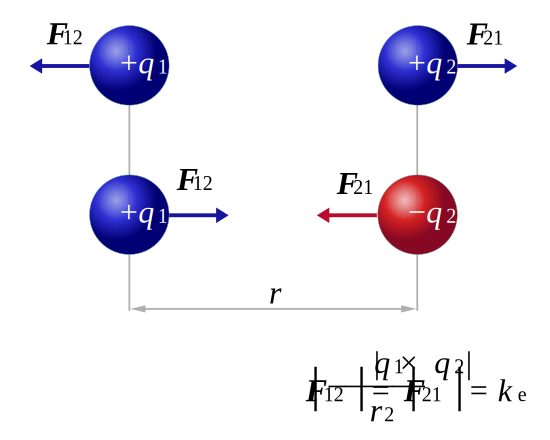
\includegraphics[scale=0.7]{CoulombsLaw}

    \caption{Signos en la Ley de Coulomb. Créditos: Wikipedia}
    \label{fig:canon_newton}
\end{figure}

El campo eléctrico generado por una partícula de carga $q$ es
\begin{align}
      \boldsymbol{E} =& k \frac{q}{r^3}\boldsymbol{r}\,,
\end{align}

% --- Inicio del código LaTeX para insertar ---

\begin{figure}[h!]
    \centering
    % Usamos minipage para colocar las dos figuras una al lado de la otra
    \begin{minipage}{0.48\textwidth}
        \centering
        % --- FIGURA IZQUIERDA: Carga Negativa ---
        \begin{tikzpicture}[
            scale=1.2, font=\large,
            charge/.style={circle, shade, ball color=blue, minimum size=1cm},
            equipotential/.style={dashed, green!50!black},
            fieldline/.style={->, >=Stealth, thick, red},
        ]
            % --- Dibujar la carga negativa en el centro ---
            \node[charge] at (0,0) {\textbf{--}};
            
            % --- Dibujar las líneas equipotenciales ---
            \foreach \r in {1, 2, 3} {
                \draw[equipotential] (0,0) circle (\r);
            }
            
            % --- Dibujar las líneas del campo eléctrico (hacia adentro) ---
            \foreach \angle in {0, 45, 90, 135, 180, 225, 270, 315} {
                \draw[fieldline] (\angle:3.5) -- (\angle:0.5);
            }
            
            % --- Añadir etiquetas ---
            \node[green!50!black, font=\small] at (0, 2.2) {Equipotencial};
            \node[red, font=\small, rotate=-45] at (45:2.5) {Campo $\vec{E}$};
        \end{tikzpicture}
        \caption*{a) Carga Negativa: Las líneas de campo apuntan radialmente hacia adentro.}
    \end{minipage}\hfill
    \begin{minipage}{0.48\textwidth}
        \centering
        % --- FIGURA DERECHA: Carga Positiva ---
        \begin{tikzpicture}[
            scale=1.2, font=\large,
            charge/.style={circle, shade, ball color=red, minimum size=1cm},
            equipotential/.style={dashed, green!50!black},
            fieldline/.style={->, >=Stealth, thick, blue},
        ]
            % --- Dibujar la carga positiva en el centro ---
            \node[charge] at (0,0) {\textbf{+}};
            
            % --- Dibujar las líneas equipotenciales ---
            \foreach \r in {1, 2, 3} {
                \draw[equipotential] (0,0) circle (\r);
            }
            
            % --- Dibujar las líneas del campo eléctrico (hacia afuera) ---
            \foreach \angle in {0, 45, 90, 135, 180, 225, 270, 315} {
                \draw[fieldline] (\angle:0.5) -- (\angle:3.5);
            }

            % --- Añadir etiquetas ---
            \node[green!50!black, font=\small] at (0, 2.2) {Equipotencial};
            \node[blue, font=\small, rotate=45] at (45:2.5) {Campo $\vec{E}$};
        \end{tikzpicture}
        \caption*{b) Carga Positiva: Las líneas de campo apuntan radialmente hacia afuera.}
    \end{minipage}
    
    \caption{Representación de las líneas del campo eléctrico ($\vec{E}$) y las superficies equipotenciales para una carga puntual negativa y una positiva. Las líneas de campo siempre son perpendiculares a las equipotenciales.}
    \label{fig:campos_electricos}
\end{figure}

% --- Fin del código LaTeX ---


Las magnitudes correspondientes para un par de cargas $q_1$ y $q_2$ son
\begin{align}
    F =& k\frac{q_1q_2}{r^2}\,,& E=& k\frac{q_1}{r^2} \,,
\end{align}
En este caso la carga $q_2$ corresponde a una carga de prueba para el  campo $E$ generado por $q_1$

%\newpage
\subsubsection{La Cantidad de Carga en un Grupo de Electrones}




\begin{examplebox}
    \textbf{Problema:} Calcule la carga, en coulombs, transportada por 6 mil millones de electrones.
\end{examplebox}

\vspace{5mm}

% --- CORRECCIÓN FINAL Y DEFINITIVA ---
% Usamos 'tabular' para la estructura general y 'array' para las ecuaciones.
\def\arraystretch{1.5} % Aumenta el espaciado vertical de las filas
\noindent % Asegura que la tabla ocupe todo el ancho
\begin{tabular}{|p{0.45\textwidth}|p{0.45\textwidth}|}
    \hline
    \textcolor{red}{\textbf{Razonamiento}} & \textcolor{red}{\textbf{Desarrollo}} \\
    \hline
    Exprese 6 mil millones (6 billion) en notación científica. & 
    % Usamos un entorno matemático y dentro un 'array' para alinear.
    \[
    \begin{array}{r@{\,}c@{\,}l} 
        1 \text{ mil millones} &=& 1 \times 10^9 \\
        6 \text{ mil millones} &=& 6 \times 10^9
    \end{array} 
    \] \\
    \hline
    Calcule la carga, $q$, en coulombs multiplicando el número de electrones por la carga de un electrón ($-1.6 \times 10^{-19}$~C). & 
    % Usamos un entorno matemático y dentro un 'array' para alinear.
    \[
    \begin{array}{r@{\,}c@{\,}l}
        q &=& (6 \times 10^9) \times (q_e) \\
          &=& (6 \times 10^9) \times (-1.6 \times 10^{-19} \, \text{C}) \\
          &=& -9.6 \times 10^{-10} \, \text{C}
    \end{array} 
    \] \\
    \hline
\end{tabular}
\def\arraystretch{1.0} % Restablece el valor por defecto

\vspace{1cm}

\textcolor{red}{\textbf{Ejemplo resuelto: Inténtalo tú mismo 12.1.1}}
\subsubsection*{La Cantidad de Carga en un Grupo de Electrones}

\begin{tcolorbox}[colframe=red, boxrule=1.5pt]
    \textbf{Problema:} Calcule la carga, en coulombs, transportada por 4 millones de electrones.
\end{tcolorbox}

% --- Fin del código LaTeX ---

% --- Inicio del código LaTeX para insertar ---

\subsubsection{Energía Potencial Electrostática ($U_e$)}

La \textbf{energía potencial electrostática ($U_e$)} de un sistema de dos cargas es una medida de la energía almacenada en el sistema debido a su configuración espacial. Se define como el \textbf{trabajo} que una fuerza externa debe realizar para traer una de las cargas (la carga de prueba, $q_2$) desde una posición de referencia en el infinito hasta una distancia $r$ de la otra carga ($q_1$), que se mantiene fija.

\subsubsection*{La Fórmula de la Energía Potencial}
La energía potencial generada por una carga fuente $q_1$ y sentida por una carga de prueba $q_2$ separadas por una distancia $r$ es:
\begin{equation}
    \boxed{
    U_e = k \frac{q_1 q_2}{r}
    }
    \label{eq:energia_potencial_e}
\end{equation}
\textbf{Notas importantes sobre la fórmula:}
\begin{itemize}
    \item A diferencia de la Ley de Coulomb para la magnitud de la fuerza, en esta ecuación los signos de las cargas $q_1$ y $q_2$ \textbf{son cruciales} y deben incluirse en el cálculo.
    \item La energía potencial decae como $1/r$, mientras que la fuerza decae como $1/r^2$.
\end{itemize}

\subsubsection*{Análisis de la Fórmula}
El signo de la energía potencial tiene una interpretación física directa:
\begin{description}
    \item[Si $U_e > 0$ (Repulsión):] Ocurre cuando $q_1$ y $q_2$ tienen el mismo signo. Se requiere un trabajo positivo (añadir energía al sistema) para juntar las cargas contra su repulsión natural. Si se sueltan, esta energía potencial se convertirá en energía cinética a medida que se alejan.

    \item[Si $U_e < 0$ (Atracción):] Ocurre cuando $q_1$ y $q_2$ tienen signos opuestos. El propio campo eléctrico realiza el trabajo para juntar las cargas. El sistema se encuentra en un estado ``ligado'' o en un ``pozo de potencial''. Se necesitaría realizar un trabajo externo positivo para separar las cargas y llevarlas al infinito.
\end{description}

\subsubsection*{Relación con el Potencial Eléctrico (Voltaje)}
El concepto de energía potencial está íntimamente ligado al de \textbf{potencial eléctrico ($V$)}, que es una propiedad del espacio creada por la carga fuente $q_1$. El potencial eléctrico se define como la energía potencial por unidad de carga:
\[ V = \frac{U_e}{q_2} \]
El potencial eléctrico creado por una carga puntual $q_1$ a una distancia $r$ es:
\[ V = k \frac{q_1}{r} \]
Con esta definición, podemos encontrar la energía potencial de cualquier carga de prueba $q_2$ colocada en un punto con potencial $V$ simplemente multiplicando:
\begin{align}
\label{eq:qV}
U_e = q_2 V
\end{align}
Esta relación es fundamental en el análisis de circuitos y campos electrostáticos.\footnote{Formalmente, la energía potencial es el negativo del trabajo realizado por la fuerza eléctrica para mover una carga desde el infinito: $U_e(r) = -\int_\infty^r \vec{F}_e \cdot d\vec{r}' = -\int_\infty^r (k \frac{q_1 q_2}{r'^2}) dr' = k \frac{q_1 q_2}{r}$.}

\subsubsection{El electronvoltio}
La energía potencial que adquiere un electrón al moverse a través de una diferencia de potencia de \qty{1}{V} es
\begin{align*}
    U_e = & V e = \qty{1}{V}\cdot \qty{1.602176634e-19}{\C} 
     =\qty{1.602176634e-19}{\joule}
\end{align*}
Esta cantidad de energía recibe el nombre de electronvoltio
\begin{align}
    \qty{1}{eV}\equiv\qty{1.602176634e-19}{\joule}\,.
\end{align}

% --- Fin del código LaTeX ---

% --- Inicio del código LaTeX para insertar ---

\subsubsection{Ejemplo Avanzado: Energía Potencial Eléctrica en el Núcleo de Uranio}

Ver libro: Destroyer of Worlds by Frank Close \url{}

Este ejemplo ilustra la escala de las energías involucradas a nivel nuclear y la inmensa fuerza de repulsión electrostática que la ``fuerza nuclear fuerte'' debe superar para mantener el núcleo unido. Además, se usa el hecho que para grandes núcleos es la fuerza eléctrica la que fuerza la fisión nuclear y entrega la energía cinética a las partes. 

Para entender esto, podemos pensar en los nucléos de los elementos químicos como gotas de un liquido muy denso que se mantiene cohesionado por la tensión superficial. La tensión superficial, $T$, es proporcional al área de la superficie sobre el volumen. Para un esfera
\begin{align*}
    T \propto \frac{\pi r^2}{\frac{4}{3}\pi r^3}
    \propto \frac{1}{r}\,,
\end{align*}
y por consiguiente disminuye con el radio. Esto hace por ejemplo que un bebe (volumen menor) necesite más abrigo que un adulto para controlar su temperatura corporal. En el caso de los núcleos implica que las ``gotas" prefieren fusionarse para el caso de núcleos livianos y fisionarse para el caso de núcleos pesados que tienden a deformarse más facilmente cuando reciben el impacto de un neutrón, como se ilustra en la figura~\ref{fig:gotas}

\includegraphics[scale=0.7]{fusion}

\includegraphics{gotas}

\subsubsection*{El Problema}
Calcular la energía potencial eléctrica total almacenada en un núcleo de Uranio-238 (${}^{235}_{92}\text{U}$) debido a la repulsión mutua de sus 92 protones. Luego, comparar esta energía con la de sus productos de fisión para entender la idea de Lise Meitner sobre la energía liberada.

\subsubsection*{El Error del ``Doble Conteo"}
% https://www.fisicalab.com/apartado/energia-potencial-electrica
Una primera intuición podría ser calcular la energía de un protón debida a los otros 91 y luego multiplicar por el número total de protones (92). Esto llevaría a una fórmula incorrecta de la forma $U_e \propto k \frac{(92e)(91e)}{R}$. Sin embargo, este método es erróneo porque cuenta la interacción de cada par de protones dos veces. La energía total de un sistema de cargas es el trabajo necesario para ensamblarlo, sumando la energía de cada \textbf{par único} de interacciones. Para un sistema complejo como un núcleo, la mejor aproximación es tratarlo como una esfera de carga uniforme.

\subsubsection*{Cálculo de la Energía Potencial Total del Núcleo de Uranio}
La energía potencial electrostática de una esfera de radio $R$ con una carga total $Q$ distribuida uniformemente es:
\begin{equation}
    U_{\text{esfera}} = \frac{3}{5} k \frac{Q^2}{R}\,.
\end{equation}
El factor 3/5 es, por tanto, un factor puramente geométrico que surge de la integración sobre el volumen de una esfera, ver apéndice~\ref{sec:3_5}. Ver también \url{https://www.feynmanlectures.caltech.edu/II_08.html}

La energía potencial es el trabajo realizado para, partiendo de un nucleón inicial, traer cada uno de los 92 protones desde el infinito. En la naturaleza éste trabajo fue realizado después de la colisión de las dos estrellas de neutrones que formaron nuestra protonebulosa planetaria. Se puede considerar entonces al Uranio como una batería natural donde se almacenó la energía gravitacional que permitió su creación. Esa energía se ha aprovechado a través de los reactores naturales que ocurrieron en momentos específicos de la historia terrestre (hace miles de millones de años) y en los reactores y bombas nucleares creados por el hombre.


\paragraph{Datos para el Uranio-235:}
\begin{itemize}
    \item Carga total, $Q = Z e = 92 \times \SI{1.602e-19}{\coulomb}$.
    \item Radio del núcleo, $R_U \approx (\SI{1.2}{\femto\meter}) \times A^{1/3} = (\SI{1.2e-15}{\meter}) \times (235)^{1/3} \approx \SI{7.41e-15}{\meter}$, donde $A$ es el número másico que es la suma de protones y neutrones en el núcleo de un átomo.
    \item Constante de Coulomb, $k \approx \SI{8.99e9}{\newton\meter\squared\per\coulomb\squared}$.
\end{itemize}

\paragraph{Cálculo:}
% --- CORRECCIÓN APLICADA AQUÍ ---
\begin{align*}
    U_{\text{Uranio}} &= \frac{3}{5} k \frac{(92e)^2}{R_U} \\
    &= \frac{3}{5} \times \num{8.99e9} \times \frac{(92 \times \num{1.602e-19})^2}{\num{7.41e-15}} \, \si{\joule} \\
    &\approx \num{1.58e-10} \, \si{\joule}
\end{align*}
Convirtiendo a Mega-electronvoltios (\SI{1}{\mega\electronvolt} = \SI{1.602e-13}{\joule}):
\[ U_{\text{Uranio}} \approx \frac{\SI{1.51e-10}{\joule}}{\SI{1.602e-13}{\joule\per\mega\electronvolt}} \approx \SI{944}{\mega\electronvolt} \]

\subsubsection*{La Genialidad de Lise Meitner: Comparando las Energías}
La idea clave de Meitner y Frisch fue comparar la energía del núcleo original con la suma de las energías de sus fragmentos de fisión, por ejemplo, Kriptón-92 (${}^{92}_{36}\text{Kr}$) y Bario-141 (${}^{141}_{56}\text{Ba}$) en la fisión
\begin{align*}
    {}^{235}_{92}\text{U} + n \to {}^{141}_{56}\text{Ba} + 
    + {}^{92}_{36}\text{Kr} + 3n\,.
\end{align*}

\paragraph{Energía de los Fragmentos:}
\begin{itemize}
    \item \textbf{Kriptón-92:} $Z=36, A=92 \implies R_{Kr} \approx \SI{5.4}{\femto\meter}$.
    \[ U_{Kr} = \frac{3}{5} k \frac{(36e)^2}{R_{Kr}} \approx \SI{200}{\mega\electronvolt} \]
    \item \textbf{Bario-141:} $Z=56, A=141 \implies R_{Ba} \approx \SI{6.2}{\femto\meter}$.
    \[ U_{Ba} = \frac{3}{5} k \frac{(56e)^2}{R_{Ba}} \approx \SI{450}{\mega\electronvolt} \]
\end{itemize}
La suma de la energía electrostática de los fragmentos es:
\[ U_{\text{fragmentos}} = U_{Kr} + U_{Ba} \approx \SI{200}{\mega\electronvolt} + \SI{450}{\mega\electronvolt} = \SI{650}{\mega\electronvolt} \]

\subsubsection*{Conclusión Final: La Fuente de la Energía de Fisión}
La diferencia entre la energía electrostática almacenada antes y después de la fisión es la energía que se libera.
\begin{itemize}
    \item Energía electrostática en el núcleo de Uranio: $\approx \SI{944}{\mega\electronvolt}$
    \item Energía electrostática en sus productos: $\approx \SI{650}{\mega\electronvolt}$
\end{itemize}
La diferencia de energía liberada es:
\[ \Delta E_{\text{electrostática}} = U_{\text{Uranio}} - U_{\text{fragmentos}} \approx \SI{944}{\mega\electronvolt} - \SI{650}{\mega\electronvolt} \approx \SI{294}{\mega\electronvolt} \]
Este valor, derivado puramente de la repulsión de Coulomb, se aproxima de manera sorprendente a la energía total liberada en una reacción de fisión (que experimentalmente es de unos \SI{200}{\mega\electronvolt}). Lise Meitner y Otto Frisch fueron los primeros en realizar este cálculo, explicando así el origen de la enorme cantidad de energía descubierta por Otto Hahn y Fritz Strassmann.

El ${}^{235}_{92}\text{U}$ existe en nuestros días en una proporción del $0.7\%$ con respecto a ${}^{238}_{92}\text{U}$. En los reactores nucleares la principal reacción de éste último es la creación de plutonio a través de la captura de neutrones
\begin{align*}
    {}^{238}_{92}\text{U} + n\to {}^{239}_{92}\text{U}\,.
\end{align*}
El nuevo nucleo ${}^{239}_{92}\text{U}$ es muy inestable y sufre un decaimiento beta rápidamente (su vida media es de unos 23 minutos). Un neutrón se convierte en un protón
\begin{align*}
    {}^{239}_{92}\text{U} \to {}^{239}_{93}\text{Np}+e^- + \overline{\nu}_e\,.
\end{align*}
El Neptunio-239 (${}^{239}_{93}\text{Np}$) también es inestable y sufre otro decaimiento beta (su vida media es de unos 2.4 días).
\begin{align*}
{}^{239}_{93}\text{Np} \to {}^{239}_{94}\text{Pu} + e^- + \overline{\nu}_e\,.   
\end{align*}
Resultado: Se ha creado un nuevo elemento, el Plutonio-239 (${}^{239}_{94}\text{Pu}$). Note que los nombres de estos dos elementos de la tabla períodica reciben su nombre a semejanza de cuando había nueve planetas y teníamos a Urano, Neptuno y Plutón. 

\subsection{Corriente eléctrica}
\begin{align}
    I =\frac{q}{t}
\end{align}

De \eqref{eq:qV},
\begin{align}
   W = U_e =& V q\nonumber\\
           = & V \frac{q}{t} t\nonumber\\
           = & V I t\,.
\end{align}

\begin{align}
    P = \frac{W}{t},,
\end{align}
Por consiguiente
\begin{align}
    P = VI,,
\end{align}
donde
\begin{itemize}
    \item $P$ es la potencia
    \item  $V$ es el Potencial eléctrico, 

  (realmente la diferencia de potencial)
    
    llamado coloquialmente el 
    \emph{Voltaje}
    \item $I$ es la corriente eléctrica
\end{itemize}

% --- Inicio del código LaTeX para insertar ---

\subsubsection{Ejemplo: Cálculo de la potencia eléctrica}
Usando  $P = V I$

Un equipo funcionando a $\qty{110}{V}$  usa una corriente de $\qty{4}{A}$.
Calcular la potencia usada por el equipo: ver tabla~\ref{tab:potencia_electrica_es}.

\begin{table}[h!]
\centering
\caption{Cálculo de la potencia eléctrica.}
\label{tab:potencia_electrica_es}
\renewcommand{\arraystretch}{1.5} % Aumenta el espaciado vertical
\begin{tabular}{|p{0.45\textwidth}|l|}
\hline
\textcolor{red}{\textbf{Razonamiento}} & \textcolor{red}{\textbf{Desarrollo}} \\
\hline
Identificar la relación necesaria para resolver el problema. & 
    $\displaystyle P = VI$ \\
\hline
Identificar los valores requeridos de la pregunta, sustituir y calcular. & 
    % Usamos un entorno align* dentro de un minipage para evitar errores
    \begin{minipage}[t]{0.45\textwidth}
    \[\begin{aligned}
        P &= VI \\
          &= 110 \times 4 \\
          &= \SI{440}{\watt}
    \end{aligned}\]
    \end{minipage} \\
\hline
\end{tabular}
\end{table}

\subsubsection{Consumo de energía}
Considere la etiqueta para el consumo de energía de un electrodoméstico mostrada en la figura~\ref{fig:nevera}. Calcule la potencia utilizada por el electrodoméstico.

\begin{figure}[h!]
    \centering
    \includegraphics[scale=0.3]{consumo}
    \caption{Consumo de energía de una nevera}
    \label{fig:nevera}
\end{figure}

\begin{align*}
    \text{P} = &{34.7}{\frac{\cancel{\text{kW}}\cancel{\text{h}}}{\cancel{\text{mes}}}}
    \left(\frac{\qty{1}{\cancel\month}}{\qty{720}{\cancel\hour}}\right)\frac{\qty{1000}{\watt}}{1\,\cancel{\text{kW}}}\\
    =& \qty{48}{\watt}
\end{align*}

La correspondiente corriente es
\begin{align*}
    I =& \frac{P}{V}\\
     = &\frac{\qty{48}{\watt}}{\qty{110}{\volt}}\\
       =& \qty{0.44}{\ampere}\,.
\end{align*}

% --- Inicio del código LaTeX para insertar ---

\subsubsection{Ejemplo: Cálculo de la Potencia Media a partir de la Factura de Servicios}

\paragraph{Enunciado del Problema:}
Si la cuenta de servicios de un hogar registra en un mes un consumo de energía de \qty{191}{\kilo\watt\hour}, ¿cuál fue la potencia media utilizada por la casa durante ese mes?

\subsubsection*{Solución Detallada}

\paragraph{1. Entender los Conceptos:}
Este problema nos pide encontrar la \textbf{potencia media}, que es la tasa constante a la que se habría consumido energía durante el mes. La factura nos proporciona la \textbf{energía total} consumida.
\begin{itemize}
    \item Energía Total Consumida, $U_e = \qty{191}{\kilo\watt\hour}$.
    \item Potencia Media, $P = \text{?}$
\end{itemize}

\paragraph{2. Fórmula de Relación:}
La relación fundamental entre energía, potencia y tiempo es $E = P \times t$. Para encontrar la potencia media, despejamos la fórmula:
\[ P = \frac{U_e}{t} \]

\paragraph{3. Calcular el Tiempo Total en Horas:}
Necesitamos el número total de horas en un mes. Asumiremos un mes promedio de 30 días y usaremos factores de conversión en modo fraccionario.
\begin{align*}
    t &= \qty{30}{días} \times \left( \frac{\qty{24}{horas}}{\qty{1}{día}} \right) \\
      &= \qty{720}{horas}
\end{align*}

\paragraph{4. Calcular la Potencia Media:}
Ahora, aplicamos la fórmula sustituyendo la energía y el tiempo total:
\[ P_{\text{media}} = \frac{\qty{191}{\kilo\watt\hour}}{\qty{720}{h}} \]
Las unidades de horas (h) en el numerador y el denominador se cancelan, dejándonos con kilovatios (kW):
\[ P_{\text{media}} \approx \qty{0.2653}{\kilo\watt} \]

\paragraph{5. Convertir a Watts (W):}
Para una interpretación más intuitiva, convertimos el resultado a vatios.
\begin{align*}
    P_{\text{media}} &= \qty{0.2653}{\kilo\watt} \times \left( \frac{\qty{1000}{W}}{\qty{1}{kW}} \right) \\
                     &\approx \qty{265.3}{\watt}
\end{align*}

\subsubsection*{Conclusión}
La potencia media consumida por la casa durante ese mes fue de aproximadamente \textbf{\qty{265}{\watt}}. Esto es equivalente al consumo continuo de, por ejemplo, un refrigerador moderno y varios dispositivos electrónicos pequeños funcionando las 24 horas del día.

% --- Fin del código LaTeX ---

% --- Fin del código LaTeX ---

\subsection{Magnetismo}

% --- Inicio del código LaTeX para insertar (versión simple) ---

El \textbf{campo magnético ($\boldsymbol{B}$)} es una cantidad vectorial, ya que tiene tanto una magnitud como una dirección.

La intensidad, o magnitud del vector, del campo magnético está en unidades de \textbf{tesla (T)} y se denota con la variable $B$.

Un imán genera un campo magnético de tipo dipolar similar al campo eléctrico que generan dos partículas cargadas de cargas opuestas como se muestra en la figura~\ref{fig:magnetismo}

\begin{figure}[h!]
    \centering
    \includegraphics[scale=0.45]{dipolar}
    \caption{Campo dipolar}
    \label{fig:magnetismo}
\end{figure}

% --- Fin del código LaTeX ---

\subsection{Electromagnetismo}
Cuando una carga eléctrica se mueve o rota genera un campo magnético. 

En la ley de Ampere la corriente eléctrica que se mueve por un alambre, genera un campo magnético concéntrico, como se muestra en la figura~\ref{fig:ampere}  dado por la Ley de Ampere:
\begin{align*}
    B = \frac{\mu_0 I}{2\pi r}\,, 
\end{align*}
donde
\begin{itemize}
    \item $B$ es la magnitud del campo magnético (en T)
    \item $\mu_0 = \qty{1.257e-6}{NA^{-2}}$ es la permeabilidad del vacío 
    \item $I$ es la corriente (en A)
    \item $r$ es la distancia desde el alamabre (en m)
\end{itemize}

\begin{figure}[h!]
    \centering
    \includegraphics[scale=0.7]{ampere}
    \caption{Ley de Ampere}
    \label{fig:ampere}
\end{figure}
% --- Fin del código LaTeX ---

Cuando una carga de prueba, $q$, se mueve con un velocidad $\boldsymbol{v}$ en presencia de un campo magnético $\boldsymbol{B}$, se genera una fuerza dada por
\begin{align}
    \boldsymbol{F} = q \boldsymbol{v}\times \boldsymbol{B}
\end{align}
con magnitud
\begin{align}
    F = q v B\sin\theta\,,
\end{align}
donde $\theta$ es el ángulo formado entre los vectores $\boldsymbol{v}$ y $\boldsymbol{B}$. Para obtener  la dirección del vector de fuerza, 
los vectores $\boldsymbol{v}$, $\boldsymbol{B}$ y $\boldsymbol{F}$ conforman una tripleta de mano derecha (ver figura~\ref{fig:manoderecha}) lo cual quiere decir que si el dedo meñique con la mano extendida señala la dirección de la velocidad, al enrollar la mano buscando la dirección del vector del campo magnético, el dedo pulgar indica la dirección de la fuerza resultante.


La magnitud de la fuerza que la corriente $I_1$ ejerce sobre una carga $q_2$ que fluye con la corriente $I_2$ a una velocidad $\boldsymbol{v}$, para recorrer la distancia $L$ en un tiempo $t$, está ilustrada en la figura~\ref{fig:alambres}

\begin{figure}
    \centering
    \includegraphics[scale=0.7]{alambres}
    \caption{Fuerza  sobre una partícula con carga $q_2$ que se mueve a velocidad $\boldsymbol{v}$ sometida a un campo magnético $\boldsymbol{B}$}
    \label{fig:alambres}
\end{figure}


\begin{align*}
F_2 =& q_2 v B_1\\
=& q_2\frac{L}{t} B_1\\
=& \frac{q_2}{t} L B_1\\
=& I_2 L B_1\,.
\end{align*}

Reemplazando la magnitud del campo magnético 
a una distancia $r$ del alambre con corriente $I_1$ (donde se encuentra el alambre con corriente $I_2$) dado por

\begin{align*}
    B_1 = \frac{\mu_0 I_1}{2\pi r}\,,
\end{align*}

tenemos que la magnitud fuerza por unidad de longitud que ejerce $I_1$ sobre $I_2$ es

\begin{align*}
    \frac{F_2}{L} = \frac{\mu_0 I_1 I_2}{2\pi r}\,,
\end{align*}

en la dirección hacia el cable con corriente $I_1$, como se muestra en la figura.

De aquí observamos que el campo magnético es una fuerza temporaloide que varía con el inverso del tiempo al cuadrado, y además, quedan claro las unidades de 
\begin{align*}
    \left[\mu_0\right] = \unit{N A^{-2}}
\end{align*}

En general, para encontrar la fuerza actuando sobre un conductor cuando la corriente se mueve a un ángulo  $\theta$ con el vector de campo magnético, esta dada por
\begin{equation}
    F = L I B \sin\theta\,,
\end{equation}
donde
\begin{itemize}
    \item $F$ es la fuerza sobre el conductor ($\unit{N}$)
    \item $L$ es la longitud del conductor ($\unit{\m}$)
    \item $I$ es la corriente en el conductor ($\unit{A}$)
    \item $B$ es la intensidad del campo magnético ($\unit{T}$)
    \item $\theta$ es el ángulo entre el campo magnético y el conductor.
\end{itemize}

\subsection{Campo magnético alrededor de un solenoide}  

Si se colocan muchas espiras una al lado de la otra, sus campos se suman y el efecto es mucho más intenso. Esto se logra fácilmente enrollando muchas vueltas de alambre en una bobina denominada solenoide. El campo alrededor del solenoide es similar al campo alrededor de un imán de barra normal. La dirección del campo magnético total se puede determinar considerando el campo alrededor de cada espira y, a su vez, el campo alrededor del alambre portador de corriente que forma la espira. La dirección del campo del solenoide depende de la dirección de la corriente en el alambre que lo compone.

Como se muestra en la figura~\ref{fig:solenoide}, el solenoide tiene el polo norte a la izquierda y el sur a la derecha. Una brújula debería apuntar en la dirección que se indica en la figura~\ref{fig:solenoide}.

\begin{figure}
    \centering
    \includegraphics[scale=0.6]{solenoide}
    \includegraphics[scale=0.3]{solenoide2}
    \caption{Campo magnético generado por la corriente circulando por un solenoide}
    \label{fig:solenoide}
\end{figure}

Un electroimán, como su nombre lo indica, funciona con electricidad. Su funcionamiento se basa en que una corriente eléctrica produce un campo magnético alrededor de un alambre portador de corriente. Si el conductor se enrolla en una serie de bobinas para formar un solenoide, el campo magnético se concentra dentro de las bobinas. Cuantas más bobinas, más fuerte es el campo magnético y, por lo tanto, más fuerte es el electroimán.
El campo magnético se puede intensificar aún más enrollando las bobinas alrededor de un núcleo. Normalmente, los átomos en materiales como el hierro apuntan en direcciones aleatorias y sus campos magnéticos individuales tienden a cancelarse entre sí. Sin embargo, el campo magnético producido por las bobinas enrolladas alrededor de un núcleo de hierro obliga a los átomos dentro del núcleo a apuntar en una sola dirección. Sus campos magnéticos individuales se suman, creando un campo magnético más fuerte. Esto es similar al concepto de fabricar un imán permanente.
La intensidad de un electroimán también se puede cambiar variando la cantidad de corriente eléctrica que fluye a través de él.
La dirección de la corriente crea polos en el electroimán. Los polos de un electroimán se pueden invertir invirtiendo la dirección de la corriente eléctrica.
Hoy en día, los electroimanes se utilizan directamente para levantar objetos pesados, como interruptores y relés, y como una forma de crear nuevos imanes permanentes al alinear los átomos dentro de materiales magnéticos.

La Ley de Ampère puede extenderse para calcular el campo magnético que rodea a un solenoide. El campo magnético en un punto bien adentro del solenoide es uniforme e independiente de la longitud o el diámetro del solenoide. En su lugar, depende del número de vueltas de la bobina ($N$) por unidad de longitud (
$L$) del solenoide. Esto se muestra en la siguiente ecuación:
\begin{align*}
    B = \frac{\mu_0 N I}{L}\,,
\end{align*}
donde $N$ es el número de vueltas por unidad de longitud $L$. El campo magnético es independiente de la longitud total del solenoide.

Esto significa que aumentar el número de vueltas de un solenoide se puede utilizar para incrementar la intensidad de su campo magnético (es decir, 
$B \propto N$). Es importante tener en cuenta que este es el número de vueltas por unidad de longitud. Por lo tanto, dos solenoides con la misma corriente pero diferentes longitudes pueden tener la misma intensidad de campo magnético. Por ejemplo, el solenoide A puede tener 100 vueltas en un metro, mientras que el solenoide B tiene 50 vueltas en 0.5 m, pero con la misma corriente, ambos producirán la misma intensidad de campo magnético.

Los solenoides se pueden utilizar para generar campos magnéticos casi uniformes, similares a los campos producidos por un imán de barra. Existen muchas aplicaciones prácticas para los solenoides, como en electroimanes, generación y distribución de energía, y motores eléctricos

\subsubsection{Ejemplo: magnitud del campo magnético en un solenoide}

% --- Inicio del código LaTeX para insertar ---

\subsubsection*{Cálculo del Campo Magnético en un Solenoide}

Un solenoide de longitud $\qty{1}{\m}$ con $N = 10$ vueltas lleva una corriente de $\qty{10}{A}$.

\paragraph{Pregunta:}
a) ¿Cuál es el campo magnético creado por esta corriente en un punto bien adentro del solenoide? (ver tabla~\ref{tab:campo_solenoide})


\begin{table}[h!]
\centering
\caption{Pasos para calcular el campo magnético en un solenoide.}
\label{tab:campo_solenoide}
\renewcommand{\arraystretch}{2.0} % Aumenta el espaciado vertical
\begin{tabular}{|p{0.5\textwidth}|l|}
\hline
\textcolor{red}{\textbf{Razonamiento}} & \textcolor{red}{\textbf{Desarrollo}} \\
\hline
Recordar la fórmula utilizada para calcular el campo magnético en un solenoide. & 
    $\displaystyle B = \frac{\mu_0 N I}{L}$ \\
\hline
Determinar qué valores usar, en unidades del SI. & 
    % Usamos un entorno align* dentro de un minipage para evitar errores
    \begin{minipage}[t]{0.45\textwidth}
    \[\begin{aligned}
        \mu_0 &= \SI{1.257e-6}{\tesla\meter\per\ampere} \\
        I &= \SI{10}{\ampere} \\
        N &= 10 \\
        L &= \SI{1}{\meter}
    \end{aligned}\]
    \end{minipage} \\
\hline
Sustituir los valores conocidos en la ecuación. & 
    $\displaystyle B = \frac{\num{1.257e-6} \times 10 \times 10}{1}$ \\
\hline
Resolver para el campo magnético $B$. & 
    % Usamos \num para el número y \si para la unidad por separado
    $\displaystyle B \approx \SI{1.3e-4}{\tesla}$ \\
\hline
\end{tabular}
\end{table}

% --- Fin del código LaTeX ---

\subsection{Ley de inducción de Faraday}

Un campo magnético variable con el tiempo, induce un campo eléctrico que varía con el tiempo también. Esto ocurre por ejemplo cuando un imán permanente entra y sale de un solenoide, como se ilustra en la figura~\ref{fig:faraday}

\begin{figure}
    \centering
    \includegraphics[scale=0.6]{faraday}
    \caption{Ley de inducción de Faraday}
    \label{fig:faraday}
\end{figure}

La corriente debe inducir un campo magnético dentro del solenoide, en la dirección opuesta a la dirección de movimiento del campo magnético inicial. Es de anotar que el mismo efecto se consigue con el imán en reposo y el solenoido entrando y saliendo del imán.

Un motor de un carro eléctrico funciona mediante la interacción entre imanes permanentes y un solenoide. Cuando se deja de acelerar y el carro sigue en movimiento, la rotación de las ruedas hace girar los componentes del motor, generando un campo magnético variable con el tiempo a través del solenoide. Según la Ley de inducción de Faraday, esto induce una corriente eléctrica que recarga la batería. Además, como indica el texto, esta corriente inducida genera su propio campo magnético en una dirección opuesta a la dirección de movimiento; esta oposición al giro actúa como una resistencia física, creando el efecto conocido como \emph{frenado regenerativo}. Ver fig~\ref{fig:ec}

\begin{figure}
    \centering
    \includegraphics[scale=0.3]{ec}
    \caption{Frenado regenerativo en carro eléctrico. Créditos: \url{
https://doi.org/10.3390/en16145303}}
    \label{fig:ec}
\end{figure}

\subsubsection{Ejemplo: Estufas de inducción}

A diferencia de una estufa convencional de gas o eléctrica que calienta mediante calor radiante desde una fuente caliente, una estufa de inducción calienta a través de la olla de metal en la que se está cocinando la comida. Una bobina de alambre de cobre se coloca dentro de la encimera. El suministro de electricidad de corriente alterna (CA) produce un campo magnético cambiante en la bobina. Esto induce una corriente  en la olla de metal conductora. La resistencia del metal en la olla, por la que fluye la corriente, transforma la energía eléctrica en calor y cocina la comida.

\subsection{Ecuaciones de Maxwell}
La contribución final de Maxwell fue la de simetrizar las ecuaciones del electromagnetismo para permitir también que un campo eléctrico que cambie con el tiempo induzca un campo magnético variable con el tiempo. Cómo a su vez un campo magnético variable con el tiempo vuelve a inducir un campo eléctrico variable con el tiempo en un proceso que se repite a la velocidad de la luz. Por consiguiente, la principal predicción de las ecuaciones de Maxwell es la  generación de las ondas electromagnéticas.


\subsection{Ejemplo del Aporte de Maxwell: La Corriente de Desplazamiento}



El aporte crucial de Maxwell, que establece que un campo eléctrico variable induce un campo magnético, se puede ilustrar sin necesidad de cálculo avanzado, analizando simplemente qué sucede cuando cargamos un condensador de placas paralelas.

\begin{figure}
    \centering
    
\begin{tikzpicture}[
    scale=1.2,
    >=Latex,
    % Estilo para el campo magnético (flechas azules curvadas)
    BField/.style={
        draw=blue!80!black, 
        thick, 
        decoration={markings, mark=at position 0.6 with {\arrow{>}}},
        postaction={decorate}
    },
    % Estilo para el campo eléctrico (flechas naranjas)
    EField/.style={
        draw=orange!90!black, 
        thick, 
        ->
    }
]

    % --- 1. EL CIRCUITO EXTERNO ---
    % Coordenadas base
    \coordinate (A) at (0,2);   % Placa izquierda
    \coordinate (B) at (3,2);   % Placa derecha
    \coordinate (TopLeft) at (-2,2);
    \coordinate (BotLeft) at (-2,0);
    \coordinate (BotRight) at (5,0);
    \coordinate (TopRight) at (5,2);

    % Cables y Componentes
    \draw[thick] (A) -- (TopLeft) -- (BotLeft) 
        to[battery1, l=$\mathcal{E}$] (0,0) 
        to[nos, l=Switch] (2,0) -- (BotRight) -- (TopRight) -- (B);

    % Etiqueta de Corriente I (real) en el cable
    \draw[->, thick, red!80!black] (-1.5, 2.2) -- (-0.5, 2.2) node[midway, above] {$I$};
    \draw[->, thick, red!80!black] (3.5, 2.2) -- (4.5, 2.2) node[midway, above] {$I$};

    % --- 2. EL CONDENSADOR (Placas paralelas en perspectiva) ---
    % Placa Izquierda (Anodo +)
    \begin{scope}[shift={(0,2)}, rotate=90]
        \draw[thick, fill=gray!30] (0,0) ellipse (1.5 and 0.2);
        \node at (0.4, 0.4) {\footnotesize $+$}; 
        \node at (-0.4, 0.4) {\footnotesize $+$};
        \node at (0, -0.4) {\footnotesize $+$};
    \end{scope}

    % Placa Derecha (Catodo -)
    \begin{scope}[shift={(3,2)}, rotate=90]
        \draw[thick, fill=gray!30] (0,0) ellipse (1.5 and 0.2);
        \node at (0.4, 0.4) {\footnotesize $-$}; 
        \node at (-0.4, 0.4) {\footnotesize $-$};
        \node at (0, -0.4) {\footnotesize $-$};
    \end{scope}

    % --- 3. EL APORTE DE MAXWELL (En el vacío) ---
    
    % Campo Eléctrico Variable (E) - Flechas Naranjas
    \foreach \y in {2.8, 2.4, 2.0, 1.6, 1.2} {
        \draw[EField] (0.2, \y) -- (2.8, \y);
    }
    \node[orange!90!black, fill=white, inner sep=1pt] at (1.5, 2.5) {$\vec{E}(t)$ variable};

    % Campo Magnético Inducido (B) - Anillos Azules
    % Representan la "Corriente de Desplazamiento"
    
    % Anillo exterior
    \draw[BField] (1.5, 2) ellipse (0.5 and 1.1);
    \node[blue!80!black, right] at (1.6, 1.0) {$\vec{B}$ inducido};

    % Anillo interior (para dar efecto 3D)
    \draw[BField, opacity=0.6, thin] (1.5, 2) ellipse (0.25 and 0.55);

    % --- 4. ETIQUETAS EXPLICATIVAS ---
    
    % Etiqueta inferior explicativa
    \node[align=center, font=\small] at (1.5, -1.5) {
        \textbf{Paradoja Resuelta:}\\
        En el vacío no hay cables, pero el cambio
        del campo eléctrico $\boldsymbol{E}$\\ genera un campo
        magnético $\boldsymbol{B}$, cerrando el circuito.
    };

    % Flecha indicando la zona de corriente de desplazamiento
    \draw[<-, thick, gray] (1.5, 0.8) -- (1.5, 0.05) node[below] {Corriente de Desplazamiento ($I_d$)};

\end{tikzpicture}
    \caption{$E(t)$}
    \label{fig:ET}
\end{figure}


\textbf{El Problema de la Corriente Interrumpida:}
Imagina un circuito simple donde una batería carga un condensador. La corriente eléctrica ($I$) fluye por el cable, acumulando cargas en las placas.
\begin{itemize}
    \item Alrededor del cable, sabemos que la corriente genera un campo magnético (Ley de Ampère).
    \item Pero, ¿qué pasa en el espacio vacío entre las placas? Allí no hay cables ni electrones moviéndose ($I=0$). Según la física anterior a Maxwell, el campo magnético debería desaparecer abruptamente en ese espacio.
\end{itemize}
Sin embargo, la naturaleza no funciona así: experimentalmente se detecta un campo magnético entre las placas idéntico al que hay alrededor del cable.

\textbf{La Solución Algebraica:}
Veamos qué está cambiando entre las placas para imitar a una corriente.
Sabemos que el campo eléctrico ($E$) entre dos placas de área $A$ está relacionado con la carga acumulada ($Q$) por la fórmula:
\begin{equation}
    E = \frac{Q}{\epsilon_0 A}
\end{equation}
Si despejamos la carga $Q$, obtenemos:
\begin{equation}
    Q = \epsilon_0 A E
\end{equation}
Sabemos que la corriente eléctrica ($I$) se define como la cantidad de carga que fluye en un tiempo determinado ($t$). Si dividimos la ecuación anterior por el tiempo, recuperamos la corriente:
\begin{equation}
    I = \frac{Q}{t} = \epsilon_0 A \frac{E}{t}
\end{equation}
Aquí está la clave de Maxwell. El término $A \times E$ se conoce como \textbf{Flujo Eléctrico} ($\Phi_E$). Por lo tanto:
\begin{equation}
    I = \epsilon_0 \frac{\Phi_E}{t}
\end{equation}
\textbf{Interpretación Física:}
Aunque no hay electrones cruzando el vacío, el \textbf{cambio del flujo eléctrico en el tiempo} ($\Phi_E / t$) se comporta matemáticamente igual que una corriente.
Maxwell llamó a este término \textbf{Corriente de Desplazamiento}.

\textbf{Conclusión:}
Maxwell corrigió la ley de Ampère estableciendo que el magnetismo tiene dos fuentes posibles:
1. Una corriente eléctrica real (cargas en movimiento).
2. Un campo eléctrico variable (cambio de flujo eléctrico).

Este ``eslabón perdido" permite que un campo eléctrico cambiante cree uno magnético, y viceversa, permitiendo que la energía viaje a través del espacio vacío como una onda electromagnética.




\subsection{Ondas electromagnéticas}
Es de anotar que así como cargas en movimiento (a velocidad constante) generan un campo magnético, en general cargas aceleradas (velocidad cambiando con el tiempo) generan ondas electromagnéticas. Por lo tanto una partícula cargada negativa orbitando una carga positiva, por ejemplo, pierde constantemente energía por la emisión de ondas electromagnéticas debido a la aceleración por la órbita.



A continuación el espectro de ondas electromagnéticas, ver figura~\ref{fig:em}.

\begin{figure}
    \centering
    \includegraphics[scale=0.25]{em}
    \caption{Espectro electromagnético}
    \label{fig:em}
\end{figure}


\subsection{Generación Controlada de Ondas: La Antena}

La predicción fundamental de las ecuaciones de Maxwell es que una carga eléctrica que se acelera debe irradiar energía en forma de ondas electromagnéticas. Para generar estas ondas de manera útil y controlada (como en la radio o el Wi-Fi), no utilizamos descargas aleatorias, sino un dispositivo que mueve las cargas rítmicamente: la \textbf{antena}.

El montaje más sencillo para entender este proceso es la \textbf{antena dipolo} conectada a un generador de corriente alterna (oscilador), como se ilustra en la figura~\ref{fig:antena}

\begin{figure}
    \centering

\begin{tikzpicture}[scale=1.5, >=Latex]

    % Definición de colores consistentes con el texto
    \definecolor{Ecolor}{RGB}{255,140,0} % Naranja para Campo Eléctrico
    \definecolor{Bcolor}{RGB}{0,100,255} % Azul para Campo Magnético

    % --- 1. EL MONTAJE (Antena y Oscilador) ---
    
    % Símbolo del Oscilador (Fuente CA)
    \draw[fill=white, thick] (-1, 0) circle (0.35);
    \node at (-1, 0) {\large $\sim$};
    \node[below, font=\scriptsize, align=center] at (-1, -0.4) {Oscilador\\(Fuente CA)};
    
    % Cables de conexión
    \draw[thick] (-0.65, 0.1) -- (0, 0.1);
    \draw[thick] (-0.65, -0.1) -- (0, -0.1);

    % Varillas de la Antena (Líneas gruesas grises)
    \draw[line width=4pt, gray!60] (0, 0.15) -- (0, 1.8); % Varilla Superior
    \draw[line width=4pt, gray!60] (0, -0.15) -- (0, -1.8); % Varilla Inferior
    
    % Cargas en los extremos (Instántanea en el tiempo)
    \node[circle, fill=red!10, draw=red, inner sep=2pt] at (0, 1.6) {\scriptsize $+$};
    \node[circle, fill=blue!10, draw=blue, inner sep=2pt] at (0, -1.6) {\scriptsize $-$};
    
    % Flechas de Corriente (I)
    \draw[->, thick, black] (-0.3, 0.4) -- (-0.3, 1.0) node[midway, left, font=\footnotesize] {$I(t)$};
    \draw[->, thick, black] (-0.3, -0.4) -- (-0.3, -1.0);

    % --- 2. LOS CAMPOS CERCANOS ---

    % Campo Eléctrico (E) - Arcos naranjas de + a -
    \foreach \angle in {30, 50} {
        % Arcos lado derecho
        \draw[Ecolor, ->, thick] (0, 1.6) to[out=-10-\angle, in=10+\angle] (0, -1.6);
        % Arcos lado izquierdo
        \draw[Ecolor, ->, thick] (0, 1.6) to[out=190+\angle, in=170-\angle] (0, -1.6);
    }
    \node[Ecolor, font=\bfseries] at (0.8, 1.2) {$\vec{E}$};

    % Campo Magnético (B) - Anillos azules alrededor de la corriente
    % Usamos elipses para dar perspectiva 3D
    \foreach \y in {0.8, -0.8} {
        \draw[Bcolor, thick] (0, \y) ellipse (0.5 and 0.15);
        % Punta de flecha para indicar dirección (Regla mano derecha)
        \draw[Bcolor, ->, thick] (0.01, \y-0.15) -- (0, \y-0.15);
    }
    \node[Bcolor, font=\bfseries] at (0.6, 0.5) {$\vec{B}$};
    
    % --- 3. LA ONDA VIAJERA (Representación esquemática) ---
    
    \begin{scope}[shift={(2.5,0)}]
        % Eje de propagación
        \draw[->, thick, darkgray] (0,0) -- (3.5,0) node[right, black] {Propagación ($c$)};
        
        % Onda Senoidal para E (Vertical)
        \draw[Ecolor, thick, domain=0:3.2, samples=100] plot (\x, {0.8*sin(\x*360)});
        
        % Vectores E
        \foreach \x in {0.25, 1.25, 2.25} {
            \draw[Ecolor, ->, thick] (\x, 0) -- (\x, 0.8);
        }
        \foreach \x in {0.75, 1.75, 2.75} {
            \draw[Ecolor, ->, thick] (\x, 0) -- (\x, -0.8);
        }
        
        % Vectores B (Horizontal/Perspectiva) - Simulando eje Z saliendo/entrando
        \foreach \x in {0.25, 1.25, 2.25} {
            \draw[Bcolor, ->, thick] (\x, 0) -- (\x-0.3, -0.3); % Saliendo
        }
        \foreach \x in {0.75, 1.75, 2.75} {
            \draw[Bcolor, ->, thick] (\x, 0) -- (\x+0.3, 0.3); % Entrando
        }
        
        % Etiqueta
        \node[above, font=\small, align=center] at (1.5, 1.0) {Onda\\Electromagnética};
    \end{scope}

\end{tikzpicture}

    \caption{Antena}
    \label{fig:antena}
\end{figure}



\subsubsection{El Mecanismo Físico}

El proceso se puede describir en pasos cíclicos, donde la electricidad se transforma en una onda viajera:

\begin{enumerate}
    \item \textbf{El Oscilador:} Una fuente de voltaje alterno empuja a los electrones hacia arriba y hacia abajo a lo largo de la varilla de metal de la antena. Este movimiento de vaivén implica que las cargas están acelerando y desacelerando constantemente.
    
    \item \textbf{Generación del Campo Eléctrico Variable ($E$):} 
    En un instante, el oscilador acumula cargas positivas en el extremo superior y negativas en el inferior. Esta separación de cargas crea un campo eléctrico alrededor de la antena. Como la polaridad del oscilador cambia continuamente, este campo eléctrico se invierte cíclicamente, creando una perturbación que varía con el tiempo.
    
    \item \textbf{Generación del Campo Magnético Variable ($B$):}
    El movimiento de las cargas para ir de un extremo al otro constituye una corriente eléctrica ($I$). Según la Ley de Ampère, esta corriente genera un campo magnético circular alrededor de la antena. Como la corriente oscila, el campo magnético también varía.
    
    \item \textbf{El Desprendimiento de la Onda:}
    Aquí entra en juego el aporte de Maxwell. Cerca de la antena, los campos $E$ y $B$ están ligados a las cargas. Sin embargo, a medida que los campos cambian, el campo eléctrico variable genera un campo magnético más lejos, y ese nuevo campo magnético genera un campo eléctrico aún más lejos.
    Los campos se ``auto-sostienen" y se desprenden de la antena, viajando por el espacio vacío a la velocidad de la luz.
\end{enumerate}

\subsubsection{Relación entre Frecuencia y Longitud de Onda}

La onda generada tiene una frecuencia ($f$) determinada por la rapidez con la que oscilan las cargas en la antena. Dado que la onda viaja a una velocidad constante $c$, la distancia entre dos crestas sucesivas de la onda, llamada longitud de onda ($\lambda$), se relaciona algebraicamente mediante:

\begin{equation}
    c = \lambda f
\end{equation}

Donde:
\begin{itemize}
    \item $c \approx 3 \times 10^8$ m/s (Velocidad de la luz).
    \item $\lambda$ es la longitud de onda en metros (m).
    \item $f$ es la frecuencia en Hertz (Hz o $s^{-1}$).
\end{itemize}

\textbf{Ejemplo:} Una emisora de radio FM transmite a una frecuencia de 100 MHz ($100 \times 10^6$ Hz). La longitud de la onda que emite su antena es:

\begin{equation}
    \lambda = \frac{c}{f} = \frac{3 \times 10^8 \, \text{m/s}}{100 \times 10^6 \, \text{s}^{-1}} = 3 \, \text{metros}
\end{equation}

Esto explica por qué las antenas de radio FM deben tener un tamaño del orden de metros para interactuar eficientemente con la onda, mientras que las antenas de los teléfonos móviles (frecuencias de GHz) son de pocos centímetros.

\subsection{El Colapso del Átomo Clásico: El Límite de la Física Newtoniana}

El modelo planetario del átomo, con un electrón orbitando un protón bajo la fuerza de Coulomb, presenta una contradicción fundamental cuando se combinan las leyes de Newton con el electromagnetismo de Maxwell. A continuación, demostraremos algebraicamente por qué este átomo es inestable y calcularemos su efímera existencia.

\subsubsection{La Predicción de Maxwell: Pérdida de Energía}

Como vimos en la sección anterior, una carga eléctrica acelerada debe emitir ondas electromagnéticas. Un electrón en órbita circular, aunque tenga rapidez constante, tiene una aceleración centrípeta constante. Por lo tanto, debe perder energía en forma de radiación.

Podemos deducir la fórmula para la potencia radiada ($P$) usando \textbf{análisis dimensional} (álgebra de unidades), sabiendo que la potencia depende de la constante de Coulomb ($k$), la carga ($e$), la aceleración ($a$) y la velocidad de la luz ($c$):

\begin{itemize}
    \item Buscamos unidades de Potencia: $[P] = \text{Newton} \cdot \text{m/s}$.
    \item El término eléctrico es $k e^2$, con unidades $\text{N}\cdot\text{m}^2$.
    \item Para obtener unidades de potencia, necesitamos multiplicar por algo con unidades de $1/(\text{m}\cdot\text{s})$.
    \item Combinando la aceleración ($a$) y la velocidad de la luz ($c$), la única combinación que funciona es $a^2/c^3$.
\end{itemize}

Algebraicamente, esto nos lleva a la \textbf{Fórmula de Larmor} (el factor numérico $2/3$ se obtiene mediante cálculo diferencial e integral):

\begin{equation}
    P = \frac{2}{3} \frac{k e^2 a^2}{c^3}
    \label{eq:larmor}
\end{equation}

\subsubsection{Estimación Algebraica del Tiempo de Vida}

Para estimar cuánto tiempo tarda el electrón en estrellarse contra el núcleo, podemos usar la relación simple:
\begin{equation}
    \text{Tiempo} (\Delta t) \approx \frac{\text{Energía Total Disponible } (|E|)}{\text{Tasa de Pérdida de Energía } (P)}
\end{equation}

\textbf{Paso 1: Calcular la Aceleración y la Energía Inicial}

Suponemos que el electrón comienza en el radio de Bohr, $r = a_0$. La fuerza de Coulomb proporciona la fuerza centrípeta:
\begin{equation}
    F = m a = \frac{k e^2}{r^2} \implies a = \frac{k e^2}{m r^2}
\end{equation}
Usando la ecuación~\eqref{eq:acentripeta} para la aceleración centrípeta en el movimiento circular
\begin{align*}
    \frac{v^2}{r} = \frac{ke^2}{mr^2}\,,
\end{align*}
tenemos que
\begin{align}
\label{eq:vala2}
    v^2 =\frac{ke^2}{mr}\,.
\end{align}


La energía total ($E$) es la suma de la cinética ($K$) y la potencial ($U$). Usando la ecuación anterior \eqref{eq:vala2}:
\begin{equation}
\label{eq:HE}
    E = K + U = \frac{1}{2}mv^2 - \frac{k e^2}{r} = \frac{k e^2}{2r} - \frac{k e^2}{r} = -\frac{k e^2}{2r}
\end{equation}
La energía disponible para perder (magnitud) es 
\begin{align}
\label{eq:energía}
    |E| = \dfrac{k e^2}{2r}\,.
\end{align}

\textbf{Paso 2: Sustitución en la Fórmula del Tiempo}

Sustituimos la aceleración $a$ en la ecuación de potencia (\ref{eq:larmor}) y luego usamos la fórmula del tiempo:

\begin{equation}
    P = \frac{2 k e^2}{3 c^3} \left( \frac{k e^2}{m r^2} \right)^2 = \frac{2 k^3 e^6}{3 c^3 m^2 r^4}\,.
\end{equation}
%
Ahora dividimos la energía en la ecuación~\eqref{eq:energía} por la potencia obtenida en el paso anterior:
%
\begin{equation}
    \Delta t \approx \frac{|E|}{P} = \frac{\left( \dfrac{k e^2}{2 r} \right)}{\left( \dfrac{2 k^3 e^6}{3 c^3 m^2 r^4} \right)}\,.
\end{equation}
Simplificando la fracción compleja algebraicamente (aplicando extremos y medios):
\begin{equation}
    \Delta t \approx \frac{3c^3m^2r^4ke^2}{4rk^3e^6} \,,
\end{equation}
tenemos finalmente
\begin{equation}
    \Delta t \approx \frac{3 c^3 m^2 r^3}{4 k^2 e^4}\,.
\end{equation}

\textbf{Paso 3: Cálculo Numérico}

Usando las constantes físicas conocidas:
\begin{itemize}
    \item $r \approx 5.3 \times 10^{-11}$ m (Radio de Bohr)
    \item $m \approx 9.11 \times 10^{-31}$ kg (Masa del electrón)
    \item $c \approx 3 \times 10^8$ m/s
    \item $k \approx 9 \times 10^9 \text{ N m}^2/\text{C}^2$
    \item $e \approx 1.6 \times 10^{-19}$ C
\end{itemize}

\begin{equation}
    \Delta t \approx \frac{3 (27 \times 10^{24}) (83 \times 10^{-62}) (149 \times 10^{-33})}{4 (81 \times 10^{18}) (6.5 \times 10^{-76})} \approx 4.7 \times 10^{-11} \text{ s}
\end{equation}

\textbf{Conclusión:}
Bajo las leyes de la física clásica descritas en este texto, el átomo de hidrógeno colapsaría en menos de una diezmilmillonésima de segundo. La estabilidad observada de la materia es la prueba irrefutable de que, a escalas atómicas, las leyes de Newton y Maxwell deben ser reemplazadas por una nueva física: la \textbf{Mecánica Cuántica}.

\subsection{El Límite de Velocidad Circular: Radiación de Sincrotrón}

La fórmula de Larmor ($P \propto a^2$) tiene una consecuencia drástica para el diseño de aceleradores de partículas. Nos impone un límite práctico a la energía máxima que puede alcanzar un electrón en una órbita circular.

Consideremos un electrón moviéndose en un círculo de radio $R$ con una velocidad $v$ cercana a la de la luz ($v \approx c$).

\subsubsection{El Conflicto Energético}

\begin{enumerate}
    \item \textbf{Ganancia de Energía:} En el acelerador, suministramos energía al electrón mediante campos eléctricos. Llamemos a esta potencia de entrada $P_{\text{entrada}}$.
    \item \textbf{Pérdida de Energía:} Al girar, el electrón tiene aceleración centrípeta. Según Larmor, esto implica que debe radiar energía. Esta energía perdida se llama \textbf{Radiación de Sincrotrón}.
\end{enumerate}

Para velocidades relativistas, la fórmula de Larmor debe corregirse multiplicándola por el factor de Lorentz a la cuarta potencia ($\gamma^4$). Dado que la energía total es $E = \gamma m c^2$, podemos decir que $\gamma \propto E$.

La potencia radiada ($P_{\text{rad}}$) escala de la siguiente manera:

\begin{equation}
    P_{\text{rad}} \propto \frac{E^4}{R^2 m^4}
\end{equation}

Esta relación revela tres hechos fundamentales:

\begin{itemize}
    \item \textbf{La Barrera de la Energía ($E^4$):} Si intentamos duplicar la energía del electrón ($2E$), la pérdida de energía por radiación se multiplica por $2^4 = 16$. La pérdida crece muchísimo más rápido que nuestra capacidad de suministrar energía.
    \item \textbf{El Límite de Equilibrio:} Se alcanza la energía máxima cuando la energía que inyectamos es igual a la que el electrón ``tira'' en forma de luz:
    \begin{equation}
        P_{\text{entrada}} = P_{\text{rad}} \implies \text{Velocidad Límite Constante}
    \end{equation}
    \item \textbf{La Importancia de la Masa ($1/m^4$):} Como la masa está en el denominador, las partículas ligeras radian mucho más. Un protón es unas 2000 veces más masivo que un electrón. Por lo tanto, para la misma energía, un electrón radia $2000^4$ (16 billones) de veces más que un protón.
\end{itemize}

\textbf{Conclusión:}
Es imposible acelerar electrones a energías arbitrariamente altas en un anillo circular, porque eventualmente toda la energía suministrada se disipa instantáneamente como radiación de sincrotrón (luz brillante, desde infrarrojos hasta rayos X). Por esta razón, el Gran Colisionador de Hadrones (LHC) usa protones (masivos) en lugar de electrones para alcanzar altas energías.

\subsection{Motivación: El Enigma de los Espectros Atómicos}

Tras analizar cómo una antena genera ondas de radio, surge una pregunta natural: si la materia está hecha de cargas eléctricas en movimiento (electrones orbitando núcleos), ¿deberían los átomos comportarse como antenas microscópicas?

Según la física clásica que hemos estudiado hasta ahora, la respuesta es sí. Sin embargo, la naturaleza nos muestra algo totalmente diferente, creando uno de los misterios más grandes que llevó al nacimiento de la mecánica cuántica.

\subsubsection{El Átomo como una Antena Variable}

Consideremos el modelo clásico del átomo de hidrógeno. El electrón gira alrededor del protón con una frecuencia orbital ($f_{\text{orb}}$).
\begin{itemize}
    \item Al igual que en la antena emisora, esta carga oscilante debería emitir una onda electromagnética (luz) con una frecuencia igual a su frecuencia de rotación: $f_{\text{luz}} = f_{\text{orb}}$.
    \item Como vimos en la sección sobre la inestabilidad, al emitir esta energía, el electrón pierde altura y cae hacia el núcleo.
    \item Al caer a una órbita más pequeña, por conservación de momento angular, el electrón debe girar más rápido. Esto significa que $f_{\text{orb}}$ aumenta continuamente.
\end{itemize}

\textbf{La Predicción Clásica (El ``Grito" de Luz):}
Si la física clásica fuera correcta, un átomo de hidrógeno excitado debería emitir un pulso de luz que cambia suavemente de color, barriendo todas las frecuencias desde el rojo hasta el ultravioleta y más allá, hasta el colapso final. Deberíamos ver un \textbf{espectro continuo} (un arcoíris completo).

\subsubsection{La Realidad Experimental: Las Líneas Discretas}

Cuando calentamos gas hidrógeno y hacemos pasar su luz a través de un prisma, no vemos un arcoíris. En su lugar, observamos algo sorprendente: el átomo permanece en silencio en la gran mayoría de las frecuencias y solo ``canta" en colores muy específicos.

Para el hidrógeno visible, solo aparecen cuatro líneas nítidas (la serie de Balmer):
\begin{itemize}
    \item Una línea Roja (656 nm).
    \item Una línea Verde-Azulada (486 nm).
    \item Dos líneas Violetas (434 nm y 410 nm).
\end{itemize}

Esta es la \textbf{huella digital del átomo}. La existencia de estas líneas de emisión implica que el electrón no puede caer en espiral de forma continua. En cambio, debe estar saltando instantáneamente entre ``escalones'' de energía fijos, emitiendo la diferencia exacta de energía como un paquete de luz.

Este comportamiento es imposible de explicar con las ecuaciones de Maxwell y Newton puras. Se necesita una nueva \textbf{regla} que ``congele'' al electrón en órbitas estables y solo permita transiciones específicas: el modelo de Bohr.

\section{Modelo de Bohr para el átomo de Hidrógeno}


Para resolver la paradoja de la inestabilidad del átomo, Niels Bohr propuso en 1913 un modelo que mezcla la física clásica con una nueva \textbf{regla} audaz. Bohr asumió que, de alguna manera, existen ciertas órbitas ``especiales'' donde el electrón no irradia energía.

Para encontrar estas órbitas, Bohr introdujo un postulado de \textbf{cuantización}: El momento angular ($L$) del electrón no puede tener cualquier valor, sino solo múltiplos enteros de una constante fundamental.

\subsection{Las Dos Ecuaciones Fundamentales}

Para derivar el modelo, solo necesitamos plantear un sistema de dos ecuaciones algebraicas con dos incógnitas: la velocidad ($v$) y el radio ($r$).

\textbf{1. Equilibrio de Fuerzas (Física Clásica):}
La fuerza eléctrica de atracción debe ser igual a la fuerza centrípeta para mantener la órbita circular. Cómo en la ecuación~\eqref{eq:vala2}
\begin{equation}
    \frac{m v^2}{r} = k \frac{e^2}{r^2} \implies m v^2 = \frac{k e^2}{r}.
    \label{eq:bohr_force}
\end{equation}

\textbf{2. Cuantización del Momento Angular (Nueva Física):}
El momento angular, ecuación~\eqref{eq:Leqmvr}, para una órbita circular,
\begin{align}
  L = mvr\,,
\end{align}
debe ser un múltiplo entero de la constante de Planck reducida ($\hbar = \frac{h}{2\pi}$):
\begin{equation}
    m v r = n \hbar, \quad \text{donde } n = 1, 2, 3, \dots.
    \label{eq:bohr_quant}
\end{equation}

\subsection{Derivación Algebraica del Radio de Bohr}

Nuestro objetivo es encontrar el radio $r$. Tenemos un sistema de ecuaciones.
Primero, despejamos la velocidad $v$ de la ecuación de cuantización (\ref{eq:bohr_quant}):
\begin{equation}
    v = \frac{n \hbar}{m r}.
\end{equation}
Ahora, sustituimos esta expresión de $v$ en la ecuación de fuerzas (\ref{eq:bohr_force}):
\begin{equation}
    m \left( \frac{n \hbar}{m r} \right)^2 = \frac{k e^2}{r}.
\end{equation}
Elevamos al cuadrado y simplificamos,
\begin{equation}
    m \frac{n^2 \hbar^2}{m^2 r^2} = \frac{k e^2}{r},
\end{equation}
lo que se reduce a
\begin{equation}
    \frac{n^2 \hbar^2}{m r^2} = \frac{k e^2}{r}.
\end{equation}
Multiplicamos ambos lados por $r^2$ para despejar el radio, obteniendo
\begin{equation}
    \frac{n^2 \hbar^2}{m} = k e^2 r.
\end{equation}
Finalmente, despejamos $r$. Al depender del número entero $n$, lo llamaremos $r_n$:
\begin{equation}
    r_n = \frac{n^2 \hbar^2}{m k e^2}.
\end{equation}

\textbf{Resultado:} Para el estado fundamental ($n=1$), obtenemos el \textbf{Radio de Bohr ($a_0$)}. Sustituyendo las constantes, recuperamos exactamente el valor que usamos en los problemas anteriores:
\begin{equation}
    a_0 \approx 5.29 \times 10^{-11} \text{ m}.
\end{equation}

\subsection{Derivación de los Niveles de Energía}

Ahora calculamos la energía total permitida para cada órbita.
Como vimos anteriormente en la ecuación~\eqref{eq:HE}, la energía total mecánica es
\begin{equation}
    E = -\frac{1}{2} \frac{k e^2}{r}.
\end{equation}
Sustituimos la expresión que encontramos para el radio $r_n$:
\begin{equation}
    E_n = -\frac{1}{2} k e^2 \left( \frac{1}{r_n} \right) = -\frac{1}{2} k e^2 \left( \frac{m k e^2}{n^2 \hbar^2} \right).
\end{equation}
Agrupando términos, llegamos a
\begin{equation}
    E_n = - \left( \frac{m k^2 e^4}{2 \hbar^2} \right) \frac{1}{n^2}.
\end{equation}

\textbf{Conclusión:}
Todo el término entre paréntesis es una constante. Si calculamos su valor (usando unidades de electronvoltios), obtenemos
\begin{equation}
    E_n = - \frac{13.6 \text{ eV}}{n^2}.
\end{equation}
Esto explica perfectamente el espectro de emisión del hidrógeno: los electrones solo pueden existir en estos niveles de energía discretos y la luz se emite cuando saltan de un nivel $n$ a uno inferior.

\appendix


\section*{Apendices}


\section{Movimiento Relativista y No Relativista Bajo una Fuerza Constante}
Esta sección proporciona un análisis completo del movimiento de una partícula con velocidad inicial en dos dimensiones bajo la influencia de una fuerza constante en una dirección. Primero derivamos la ecuación de movimiento completamente relativista, luego la expresamos elegantemente en términos de la energía total relativista, revelando su conexión con el Teorema del Trabajo y la Energía. Posteriormente, demostramos el principio de correspondencia mostrando cómo la ecuación relativista se reduce correctamente al caso clásico en el límite no relativista. Finalmente, para completar, derivamos la ecuación de movimiento clásica de forma independiente utilizando el Teorema del Trabajo y la Energía no relativista.

\subsection{Configuración del Problema}
Consideramos el movimiento de una partícula de masa en reposo $m$.
\begin{itemize}
    \item \textbf{Condiciones Iniciales:} En el tiempo $t=0$, la partícula está en la posición $(x_0, y_0)$ con una velocidad inicial $\boldsymbol{u}_0 = (u_{x0}, u_{y0})$.
    \item \textbf{Fuerza:} Una fuerza constante $\boldsymbol{F}$ actúa solo en la dirección y negativa: $\boldsymbol{F} = (0, -F)$, donde $F$ es una constante positiva.
\end{itemize}
En relatividad, la Segunda Ley de Newton se escribe como la tasa de cambio del momento relativista:
\[ \boldsymbol{F} = \frac{d\boldsymbol{p}}{dt}, \quad \text{donde} \quad \boldsymbol{p} = \gamma m \boldsymbol{u} \]
El factor de Lorentz, $\gamma$, depende de la velocidad total $u = \sqrt{u_x^2 + u_y^2}$:
\[ \gamma = \frac{1}{\sqrt{1 - u^2/c^2}} = \frac{1}{\sqrt{1 - (u_x^2 + u_y^2)/c^2}} \]
Esta dependencia de la velocidad total significa que el movimiento en las direcciones $x$ e $y$ está acoplado, una característica clave de la dinámica relativista.

\subsection{La Ecuación de Movimiento Relativista}

\subsection{Resolviendo para el Momento}
La ecuación vectorial $\boldsymbol{F} = d\boldsymbol{p}/dt$ proporciona dos ecuaciones escalares para las componentes del momento $p_x$ y $p_y$.
\begin{itemize}
    \item \textbf{Dirección x:} $F_x = \frac{dp_x}{dt} = 0$. Esto implica que la componente $x$ del momento se conserva:
    \[ p_x(t) = p_{x0} = \gamma_0 m u_{x0} \]
    donde $\gamma_0$ es el factor de Lorentz inicial.
    \item \textbf{Dirección y:} $F_y = \frac{dp_y}{dt} = -F$. Integrando con respecto al tiempo se obtiene:
    \[ p_y(t) = p_{y0} - Ft = \gamma_0 m u_{y0} - Ft \]
\end{itemize}




\subsection{Encontrando la Velocidad \texorpdfstring{$u_y(t)$}{uy(t)}}
Para encontrar la ecuación de movimiento para $y(t)$, primero necesitamos la velocidad $u_y(t) = dy/dt$. Podemos expresar las componentes de la velocidad en términos del momento y la energía total usando la relación relativista energía-momento $E^2 = (pc)^2 + (mc^2)^2$. Dado que $E=\gamma m c^2$, podemos encontrar $\gamma = \frac{1}{mc}\sqrt{p_x^2 + p_y^2 + m^2c^2}$. Esto conduce a:
\[ u_y(t) = \frac{p_y(t)}{\gamma(t) m} = \frac{c \, p_y(t)}{\sqrt{p_x(t)^2 + p_y(t)^2 + m^2c^2}} \]
Sustituyendo nuestras expresiones dependientes del tiempo para el momento:
\[ \frac{dy}{dt} = u_y(t) = \frac{c (p_{y0} - Ft)}{\sqrt{p_{x0}^2 + (p_{y0} - Ft)^2 + m^2c^2}} \]

\subsection{Integrando para Encontrar la Posición \texorpdfstring{$y(t)$}{y(t)}}
Integramos la velocidad $u_y(t)$ de $0$ a $t$ para encontrar el desplazamiento.
\[ y(t) - y_0 = \int_0^t \frac{c (p_{y0} - Ft')}{\sqrt{p_{x0}^2 + (p_{y0} - Ft')^2 + m^2c^2}} \, dt' \]
Esta integral se puede resolver usando una sustitución u para el término dentro de la raíz cuadrada. El resultado de la integración es:
\[ y(t) - y_0 = \frac{c}{F} \left( \sqrt{p_{x0}^2 + p_{y0}^2 + m^2c^2} - \sqrt{p_{x0}^2 + (p_{y0} - Ft)^2 + m^2c^2} \right) \]
Esto da la ecuación de movimiento relativista final para la coordenada y.

\subsection{Teorema del Trabajo y la Energía}

\begin{equation}
dW = \overline{F} \cdot d\overline{s} \label{eq:3}
\end{equation}
es el trabajo infinitesimal realizado por la fuerza $\overline{F}$ mientras la partícula sufre el desplazamiento $d\overline{s}$ a lo largo de su trayectoria. Usamos la segunda ley de Newton del movimiento
\begin{equation}
\overline{F} = \frac{d(m\overline{v})}{dt}
\end{equation}
en la ecuación (\ref{eq:3}) para obtener una expresión para el trabajo infinitesimal
\begin{align*}
dW &= \frac{d(m\overline{v})}{dt} \cdot \overline{v}dt \\
&= \frac{d}{dt}\left(\frac{1}{2}m\overline{v}\cdot\overline{v}\right)dt \\
&= d\left(\frac{1}{2}m\overline{v}^{2}\right).
\end{align*}
Dado que la cantidad escalar $\frac{1}{2}m\overline{v}^{2}$ es la energía cinética de la partícula, se sigue que
\begin{equation}
dW = dT. \label{eq:4}
\end{equation}
La ecuación (\ref{eq:4}) es la forma diferencial del teorema del trabajo y la energía: establece que el trabajo diferencial de la resultante de las fuerzas que actúan sobre una partícula es igual, en cualquier momento, al cambio diferencial en la energía cinética de la partícula. Integrando la ecuación (\ref{eq:4}) entre el punto 1 y el punto 2, correspondientes a las velocidades $\overline{v}_1$ y $\overline{v}_2$ de la partícula, obtenemos
\begin{equation}
W_{12} = \int_{1}^{2} dW = \int_{1}^{2} dT = T_2 - T_1 = \frac{1}{2}m\overline{v}_{2}^{2} - \frac{1}{2}m\overline{v}_{1}^{2}. \label{eq:5}
\end{equation}



\subsection{Formulación Energética de la Ecuación Relativista}
La ecuación anterior se puede expresar de una forma mucho más elegante y físicamente perspicaz utilizando el concepto de energía total relativista.
Sea $E_0$ la energía total inicial en $t=0$:
\[ E_0 = \sqrt{(p_{x0}^2 + p_{y0}^2)c^2 + (mc^2)^2} \]
Y sea $E(t)$ la energía total en el tiempo $t$:
\[ E(t) = \sqrt{(p_x(t)^2 + p_y(t)^2)c^2 + (mc^2)^2} = \sqrt{(p_{x0}^2 + (p_{y0}-Ft)^2)c^2 + (mc^2)^2} \]
Podemos ver que los términos en nuestra ecuación para $y(t)$ son simplemente $E_0/c$ y $E(t)/c$. Sustituyendo esto se obtiene:
\[ y(t) - y_0 = \frac{c}{F} \left( \frac{E_0}{c} - \frac{E(t)}{c} \right) \]
El factor $c$ se cancela, lo que lleva a la forma notablemente simple:
\[ \boxed{y(t) = y_0 + \frac{E_0 - E(t)}{F}} \]
Esta ecuación es una declaración directa del Teorema del Trabajo y la Energía, $F \Delta y = -\Delta E$, con la energía relativista en lugar de la energía cinética, ver más abajo.

\subsection{El Límite No Relativista (Principio de Correspondencia)}
Una teoría relativista válida debe reproducir los resultados clásicos a bajas velocidades ($u \ll c$). Mostramos esto usando la aproximación binomial para la energía total $E = \gamma mc^2$. Para velocidades pequeñas, $\gamma \approx 1 + \frac{1}{2}\frac{u^2}{c^2}$, lo que da:
\[ E \approx mc^2 + \frac{1}{2}mu^2 = (\text{Energía en Reposo}) + (\text{Energía Cinética Clásica}) \]
Aplicando esto a nuestra ecuación de movimiento basada en la energía:
\[ y(t) - y_0 = \frac{1}{F} \left[ \left(mc^2 + \frac{1}{2}mu_0^2\right) - \left(mc^2 + \frac{1}{2}mu(t)^2\right) \right] = \frac{m}{2F}(u_0^2 - u(t)^2) \]
En el límite no relativista, las velocidades son $u_x(t) = u_{x0}$ y $u_y(t) = u_{y0} - \frac{F}{m}t$. Sustituyendo esto:
\begin{align*}
y(t) - y_0 &= \frac{m}{2F} \left[ (u_{x0}^2 + u_{y0}^2) - \left(u_{x0}^2 + (u_{y0} - \frac{F}{m}t)^2\right) \right] \\
&= \frac{m}{2F} \left[ u_{y0}^2 - \left(u_{y0}^2 - 2u_{y0}\frac{F}{m}t + \frac{F^2}{m^2}t^2\right) \right] \\
&= \frac{m}{2F} \left[ 2u_{y0}\frac{F}{m}t - \frac{F^2}{m^2}t^2 \right] \\
&= u_{y0}t - \frac{F}{2m}t^2
\end{align*}
Esto produce la ecuación de movimiento clásica final:
\[ \boxed{y(t) = y_0 + u_{y0}t - \frac{F}{2m}t^2} \]
La fórmula relativista se reduce correctamente a la clásica.

\subsection{Derivación Directa del Caso No Relativista}
Como confirmación final, podemos derivar la ecuación de movimiento clásica directamente del Teorema del Trabajo y la Energía no relativista, $W_{neto} = \Delta K$.
\begin{itemize}
    \item \textbf{Trabajo Realizado:} $W_{neto} = \boldsymbol{F} \cdot \Delta\boldsymbol{r} = -F(y(t) - y_0)$.
    \item \textbf{Cambio en la Energía Cinética:} $\Delta K = K_{final} - K_{inicial} = \frac{1}{2}mu(t)^2 - \frac{1}{2}mu_0^2$.
\end{itemize}
Usando las velocidades clásicas $u_x(t) = u_{x0}$ y $u_y(t) = u_{y0} - \frac{F}{m}t$:
\[ \Delta K = \frac{1}{2}m\left[ (u_{x0}^2 + (u_{y0}-\frac{F}{m}t)^2) - (u_{x0}^2+u_{y0}^2) \right] = \frac{1}{2}m\left[ (u_{y0}-\frac{F}{m}t)^2 - u_{y0}^2 \right] \]
Estableciendo $W_{neto} = \Delta K$:
\[ -F(y(t)-y_0) = \frac{1}{2}m\left[ (u_{y0}^2 - 2u_{y0}\frac{F}{m}t + \frac{F^2}{m^2}t^2) - u_{y0}^2 \right] \]
\[ -F(y(t)-y_0) = -u_{y0}Ft + \frac{F^2}{2m}t^2 \]
Dividiendo por $-F$ se obtiene el resultado idéntico:
\[ y(t) - y_0 = u_{y0}t - \frac{F}{2m}t^2 \]







% --- INFORMACIÓN DEL TÍTULO ---
\section{Derivación de las Transformaciones de Lorentz a partir de Simetrías del Espacio--tiempo}
\label{sec:tl}
\subsection{El Enfoque de Ignatowski}
Este documento presenta una derivación de las transformaciones de Lorentz basada en principios fundamentales de simetría, en lugar de postular la constancia de la velocidad de la luz. Este enfoque, a veces llamado la derivación de Ignatowski, se basa en el Principio de Relatividad y la homogeneidad e isotropía del espaciotiempo. Mostraremos que estos principios conducen lógicamente a la existencia de una velocidad universal e invariante, que identificamos con la velocidad de la luz.

Ver \cite{Datta:2022cpw} %https://inspirehep.net/literature/2611550


\subsection{Principios Fundamentales}
La derivación se basa en tres supuestos centrales:
\begin{enumerate}
    \item \textbf{El Principio de Relatividad:} Las leyes de la física son las mismas en todos los sistemas de referencia inerciales.
    \item \textbf{Homogeneidad del Espaciotiempo:} Las leyes de la física son independientes de la posición en el espacio y el tiempo.
    \item \textbf{Isotropía del Espacio:} Las leyes de la física son independientes de la dirección.
\end{enumerate}


\subsection{Paso 1: Linealidad a partir de la Homogeneidad}
Consideremos dos sistemas de referencia inerciales, $S(x,t)$ y $S'(x',t')$, con $S'$ moviéndose a una velocidad $v$ relativa a $S$ a lo largo del eje x. Buscamos las funciones de transformación $x' = f(x,t)$ y $t' = g(x,t)$.

La homogeneidad del espaciotiempo implica que las ecuaciones de transformación deben ser \textbf{lineales}. Si no lo fueran, un movimiento uniforme en un sistema (una línea recta en un diagrama de espaciotiempo) aparecería como un movimiento acelerado en otro. Esto significaría que las leyes de la física dependerían de la elección del origen, violando la homogeneidad. Por lo tanto, la forma más general de las transformaciones debe ser lineal:
\begin{align*}
x' &= Ax + Bt \\
t' &= Dx + Et
\end{align*}
donde los coeficientes $A, B, D, E$ solo pueden depender de la velocidad relativa, $v$.

\subsection{Paso 2: Usando Cinemática Básica}
Podemos simplificar los coeficientes usando el movimiento de los orígenes de los sistemas.
\begin{itemize}
    \item El origen del sistema $S'$ ($x'=0$) se mueve con velocidad $v$ en el sistema $S$. Su posición en $S$ es por lo tanto $x=vt$. Sustituyamos esto en nuestra primera ecuación:
    \[ 0 = A(vt) + Bt \implies 0 = (Av+B)t \]
    Esto debe ser válido para todo tiempo $t$, por lo que debemos tener $B = -Av$. La transformación para $x'$ se convierte en:
    \[ x' = Ax - Avt = A(x-vt) \]
\end{itemize}
Renombremos el coeficiente $A(v)$ con la notación más familiar $\gamma(v)$.
\begin{equation} \label{eq:x_prime}
x' = \gamma(v)(x - vt)
\end{equation}

\subsection{Paso 3: Aplicando la Relatividad y la Isotropía}
El Principio de Relatividad establece que la transformación de $S'$ de vuelta a $S$ debe tener exactamente la misma forma matemática. La única diferencia es que desde la perspectiva de $S'$, el sistema $S$ se mueve con velocidad $-v$. Por lo tanto, la transformación inversa debe ser:
\begin{equation} \label{eq:x}
x = \gamma(-v)(x' + vt')
\end{equation}
Ahora, invocamos la \textbf{isotropía del espacio}. La isotropía significa que la física no debe depender de la dirección del vector velocidad. Por lo tanto, cualquier efecto físico de la transformación solo puede depender de la \textit{rapidez}, $|v|$, no de la dirección de la velocidad. Esto implica:
\[ \gamma(v) = \gamma(-v) \]
Esto simplifica nuestro par de transformaciones a:
\begin{align*}
x' &= \gamma(v)(x - vt) \\
x &= \gamma(v)(x' + vt')
\end{align*}

\subsection{Paso 4: Encontrando la Transformación del Tiempo}
Todavía necesitamos determinar la transformación para el tiempo. Podemos mostrar que debe tomar la forma simétrica:
\begin{equation} \label{eq:t_prime}
t' = \gamma(v)(t - \alpha(v) x)
\end{equation}
donde $\alpha(v)$ es alguna función de la velocidad. Por el Principio de Relatividad, la transformación inversa debe ser:
\begin{equation} \label{eq:t}
t = \gamma(v)(t' + \alpha(v) x')
\end{equation}
Nótese que la isotropía implica $\alpha(-v) = -\alpha(v)$ (debe ser una función impar).

\subsection{Paso 5: La Propiedad de Grupo y la Constante Universal}
Este es el paso crucial que reemplaza el postulado de la velocidad de la luz. Consideremos tres sistemas: $S$, $S'$ y $S''$. Sea la velocidad de $S'$ relativa a $S$ $v_1$, y la velocidad de $S''$ relativa a $S'$ $v_2$. La composición de estas dos transformaciones debe dar como resultado una transformación de la misma forma.

Sustituyendo (\ref{eq:x_prime}) y (\ref{eq:t_prime}) en (\ref{eq:x}) y (\ref{eq:t}), podemos resolver para las funciones. Un método más directo es requerir consistencia entre las transformaciones. Sustituyamos (\ref{eq:x_prime}) en (\ref{eq:x}):
\begin{align*}
x &= \gamma(v)(x' + vt') \\
x &= \gamma(v)[\gamma(v)(x-vt) + v t']
\end{align*}
Ahora sustituimos nuestra expresión para $t'$ (\ref{eq:t_prime}):
\begin{align*}
x &= \gamma(v)[\gamma(v)(x-vt) + v \gamma(v)(t - \alpha(v)x)] \\
x &= \gamma(v)^2 [ (x-vt) + v(t-\alpha(v)x) ] \\
x &= \gamma(v)^2 [ x - vt + vt - v\alpha(v)x ] \\
x &= \gamma(v)^2 x (1 - v\alpha(v))
\end{align*}
Como esto debe ser válido para cualquier $x$, debemos tener:
\[ 1 = \gamma(v)^2 (1 - v\alpha(v)) \]
Esto relaciona nuestras dos funciones desconocidas, $\gamma(v)$ y $\alpha(v)$.

A partir del argumento de la propiedad de grupo (considerando tres sistemas), se puede mostrar que la razón $\alpha(v)/v$ debe ser una constante universal, independiente del sistema de referencia. Llamemos a esta constante $K$.
\[ \frac{\alpha(v)}{v} = K \implies \alpha(v) = Kv \]
Ahora sustituimos esto de nuevo en nuestra relación de consistencia:
\[ 1 = \gamma(v)^2 (1 - v(Kv)) = \gamma(v)^2 (1 - K v^2) \]
Resolviendo para $\gamma(v)$:
\[ \boxed{\gamma(v) = \frac{1}{\sqrt{1 - K v^2}}} \]

\subsection{Paso 6: La Naturaleza Física de la Constante \texorpdfstring{$K$}{K}}
Hemos derivado la forma completa de las transformaciones basándonos únicamente en principios de simetría. La física está contenida en la constante universal $K$.
\begin{enumerate}
    \item \textbf{Caso 1: $K=0$} \\
    Si $K=0$, entonces $\gamma = 1$ y $\alpha=0$. Las transformaciones se convierten en $x' = x - vt$ y $t'=t$. Esta es la \textbf{transformación de Galileo}. En este universo, no hay límite de velocidad.

    \item \textbf{Caso 2: $K<0$} \\
    Si $K$ es negativo, sea $K = -1/R^2$. Entonces $\gamma = 1/\sqrt{1+v^2/R^2}$. Esto corresponde a transformaciones en un espacio euclidiano 4D (rotaciones). Esto es matemáticamente posible pero no describe nuestro universo.

    \item \textbf{Caso 3: $K>0$} \\
    Si $K$ es positivo, debe tener unidades de (1/velocidad$^2$). Definamos una nueva constante $c$ tal que $K = 1/c^2$. Esta constante $c$ debe ser una velocidad universal e invariante. El factor de Lorentz y las transformaciones se convierten en:
    \[ \gamma = \frac{1}{\sqrt{1 - v^2/c^2}} \]
    \[ x' = \gamma(x-vt) \]
    \[ t' = \gamma(t - \frac{v}{c^2}x) \]
    Estas son las \textbf{transformaciones de Lorentz}.
\end{enumerate}

\subsection{Conclusión}
Sin asumir nunca que la luz viaja a una velocidad constante, hemos demostrado que las simetrías fundamentales del espaciotiempo (homogeneidad e isotropía) y el principio de relatividad conducen a una conclusión sorprendente: \textbf{debe existir una velocidad universal e invariante en nuestro universo}.

Toda la evidencia experimental, desde el electromagnetismo hasta la desintegración de partículas, confirma que vivimos en un universo donde $K > 0$. Llamamos a esta velocidad universal $c$, y la identificamos con la velocidad de la luz en el vacío. La constancia de la velocidad de la luz no es una suposición separada, sino una consecuencia directa de la estructura del espaciotiempo mismo.


\section{Número Imaginario}
Definimos
\begin{align}
    i \equiv \sqrt{-1}\,.
\end{align}
Por lo tanto
\begin{align}
    i^2 = i\cdot i = (-1)^{\frac{1}{2}}(-1)^{\frac{1}{2}}=(-1)^{\frac{1}{2}+\frac{1}{2}}
    =(-1)^{\frac{1+1}{2}}= (-1)^1 = -1\,.
\end{align}
\section{Demostración de la Fórmula de Euler mediante Cálculo}
La fórmula de Euler es
    \begin{align*}
        e^{i\theta} = \cos\theta + i\sin\theta\,.
    \end{align*}

Se puede construir una prueba utilizando cálculo básico.
\begin{enumerate}
    \item Definir una función $f(\theta) = \cos\theta + i\sin\theta$.
    \item Derivar $f(\theta)$ con respecto a $\theta$:
    \[ \frac{df}{d\theta} = -\sin\theta + i\cos\theta \]
    \item Factorizar una $i$ de la derivada, usando $i^2=-1$:
    \[ \frac{df}{d\theta} = i(i\sin\theta + \cos\theta) = i f(\theta) \]
    \item Ahora tenemos una ecuación diferencial simple de primer orden: $\frac{df}{f} = i \, d\theta$.
    \item Integrando ambos lados se obtiene $\ln(f) = i\theta + C$, donde $C$ es la constante de integración.
    \item Exponenciando se obtiene $f(\theta) = e^{i\theta+C} = e^C e^{i\theta}$.
    \item Para encontrar la constante $e^C$, evaluamos la función en $\theta=0$:
    \[ f(0) = \cos(0) + i\sin(0) = 1 + 0 = 1 \]
    De nuestra solución, también tenemos $f(0) = e^C e^{i \cdot 0} = e^C$.
    \item Por lo tanto, la constante $e^C=1$, y nuestra solución final es $f(\theta) = e^{i\theta}$. Como definimos $f(\theta) = \cos\theta + i\sin\theta$, la identidad queda demostrada:
    \begin{align}
    \boxed{
        e^{i\theta} = \cos\theta + i\sin\theta\,.
        }
    \end{align}
\end{enumerate}

\section{Derivando Seno y Coseno de la Fórmula de Euler}
Una aplicación poderosa de la fórmula de Euler es expresar el seno y el coseno en términos de exponenciales complejas. Esto se logra tratando la fórmula de Euler y su conjugada como un sistema de dos ecuaciones lineales.

\subsection{El Sistema de Ecuaciones}
Comenzamos con la fórmula de Euler y una segunda versión donde $\theta$ es reemplazado por $-\theta$:
\begin{align*}
    e^{i\theta} &= \cos\theta + i\sin\theta \tag{A.1} \\
    e^{-i\theta} &= \cos(-\theta) + i\sin(-\theta) = \cos\theta - i\sin\theta \tag{A.2}
\end{align*}
La segunda ecuación utiliza la propiedad par del coseno ($\cos(-\theta)=\cos\theta$) y la propiedad impar del seno ($\sin(-\theta)=-\sin\theta$).

\subsection{Resolviendo para \texorpdfstring{$\cos\theta$}{cos(theta)}}
Para aislar $\cos\theta$, sumamos las ecuaciones (A.1) y (A.2) para eliminar los términos del seno:
\begin{align*}
    e^{i\theta} + e^{-i\theta} &= (\cos\theta + i\sin\theta) + (\cos\theta - i\sin\theta) \\
    e^{i\theta} + e^{-i\theta} &= 2\cos\theta
\end{align*}
Resolviendo para $\cos\theta$ se obtiene:
\[ \boxed{\cos\theta = \frac{e^{i\theta} + e^{-i\theta}}{2}} \]

\subsection{Resolviendo para \texorpdfstring{$\sin\theta$}{sin(theta)}}
Para aislar $\sin\theta$, restamos la ecuación (A.2) de la ecuación (A.1) para eliminar los términos del coseno:
\begin{align*}
    e^{i\theta} - e^{-i\theta} &= (\cos\theta + i\sin\theta) - (\cos\theta - i\sin\theta) \\
    e^{i\theta} - e^{-i\theta} &= 2i\sin\theta
\end{align*}
Resolviendo para $\sin\theta$ se obtiene:
\[ \boxed{\sin\theta = \frac{e^{i\theta} - e^{-i\theta}}{2i}} \]
Estas definiciones son fundamentales en muchas áreas de la física y la ingeniería, particularmente en el análisis de Fourier.

\subsection{Conexión con las Funciones Hiperbólicas}

Estas formas exponenciales son sorprendentemente similares a las definiciones de las funciones hiperbólicas:
\[ \cosh(x) = \frac{e^x + e^{-x}}{2} \quad \text{y} \quad \sinh(x) = \frac{e^x - e^{-x}}{2} \]
Por comparación directa, podemos ver la relación formal utilizada en el texto principal para la rotación de Wick.
\begin{itemize}
    \item Comparando $\cos\theta$ con $\cosh(x)$, vemos que si establecemos $x=i\theta$, obtenemos $\cosh(i\theta) = \frac{e^{i\theta} + e^{-i\theta}}{2} = \cos\theta$.
    \item Comparando $\sin\theta$ con $\sinh(x)$, vemos que $\sinh(i\theta) = \frac{e^{i\theta} - e^{-i\theta}}{2} = i \left( \frac{e^{i\theta} - e^{-i\theta}}{2i} \right) = i\sin\theta$.
\end{itemize}
Esto demuestra la profunda consistencia matemática entre las funciones trigonométricas e hiperbólicas en el plano complejo.

\subsection{La Matriz de Lorentz}
Podemos escribir la transformación $X' = \Lambda X$ como:
\[ \begin{pmatrix} t' \\ x'  \end{pmatrix} = \Lambda \begin{pmatrix} t \\ x  \end{pmatrix} \]
Inspeccionando las ecuaciones de transformación, podemos escribir la matriz $\Lambda$ primero en términos de $\gamma$ y $v$, y luego sustituir las funciones hiperbólicas:
\[
\Lambda(\xi) = \begin{pmatrix} \gamma & -v\gamma  \\ -v\gamma & \gamma  \\  \end{pmatrix}
=
\boxed{
\begin{pmatrix} \cosh\xi & -\sinh\xi  \\ -\sinh\xi & \cosh\xi  \\  \end{pmatrix}
}
\]
Esto revela que un impulso de Lorentz es una \textbf{rotación hiperbólica} en el espaciotiempo.

\section{La Rotación de Wick: Impulsos como Rotaciones Imaginarias}

La conexión con la geometría se vuelve aún más sorprendente si tratamos la rapidez como un ángulo imaginario. Este procedimiento es parte de una técnica conocida como \textbf{rotación de Wick}.

\subsection{De Funciones Hiperbólicas a Trigonométricas}
Establezcamos la rapidez $\xi$ como un ángulo imaginario, $\xi = i\theta$. Usando las definiciones de las funciones hiperbólicas en términos de exponenciales, encontramos las siguientes identidades:
\begin{align*}
    \cosh(i\theta) &= \frac{e^{i\theta} + e^{-i\theta}}{2} = \cos\theta \\
    \sinh(i\theta) &= \frac{e^{i\theta} - e^{-i\theta}}{2} = i \left( \frac{e^{i\theta} - e^{-i\theta}}{2i} \right) = i\sin\theta
\end{align*}

\subsection{La Transformación Completa en el Espaciotiempo Euclidiano}
Ahora, realicemos una rotación de Wick completa aplicando dos cambios simultáneamente:
\begin{enumerate}
    \item \textbf{Rapidez Imaginaria:} $\xi \to i\theta$
    \item \textbf{Tiempo Imaginario:} $t \to i\tau$ (y por lo tanto $t' \to i\tau'$)
\end{enumerate}
Aplicamos esto a la ecuación matricial $X'=\Lambda X$, centrándonos en las componentes $(t,x)$:
\[ \begin{pmatrix} i\tau' \\ x' \end{pmatrix} = \begin{pmatrix} \cos\theta & -i\sin\theta \\ -i\sin\theta & \cos\theta \end{pmatrix} \begin{pmatrix} i\tau \\ x \end{pmatrix} \]
Multiplicando esto se obtienen dos ecuaciones:
\begin{align*}
    i\tau' &= (\cos\theta)(i\tau) + (-i\sin\theta)(x) = i(\tau\cos\theta - x\sin\theta) \\
    x' &= (-i\sin\theta)(i\tau) + (\cos\theta)(x) = (-i^2)\tau\sin\theta + x\cos\theta = \tau\sin\theta + x\cos\theta
\end{align*}
Después de cancelar la $i$ de la primera ecuación, obtenemos el resultado final:
\[
\begin{aligned}
\tau' &= \tau\cos\theta - x\sin\theta \\
x' &= x\cos\theta + \tau\sin\theta
\end{aligned}
\]
Esto es precisamente una rotación euclidiana estándar en el plano $(\tau, x)$. En forma matricial:
\[
\boxed{
\begin{pmatrix} \tau' \\ x' \end{pmatrix} = \begin{pmatrix} \cos\theta & -\sin\theta \\ \sin\theta & \cos\theta \end{pmatrix} \begin{pmatrix} \tau \\ x \end{pmatrix}
}
\]

% --- TABLA AÑADIDA INICIO ---
\begin{table}[h!]
\centering
\caption{Resumen de la Rotación de Wick: Mapeo de un Impulso de Lorentz a una Rotación Euclidiana.}
\label{tab:wick}
\begin{tabular}{l|l|l}
\hline
\textbf{Característica} & \textbf{Espaciotiempo de Minkowski (Impulso)} & \textbf{Espaciotiempo Euclidiano (Rotación)} \\
\hline \hline
Coordenadas & $(t, x)$ & $(\tau, x)$, donde $t = i\tau$ \\
\hline
Intervalo Invariante & $s^2 = t^2 - x^2$ & $d^2 = \tau^2 + x^2$ \\
\hline
Tipo de Transformación & Rotación Hiperbólica & Rotación Circular \\
\hline
Parámetro & Rapidez, $\xi = \tanh^{-1}(v)$ & Ángulo, $\theta$ (donde $\xi = i\theta$) \\
\hline
Forma Matricial & $\begin{pmatrix} \cosh\xi & -\sinh\xi \\ -\sinh\xi & \cosh\xi \end{pmatrix}$ & $\begin{pmatrix} \cos\theta & -\sin\theta \\ \sin\theta & \cos\theta \end{pmatrix}$ \\
\hline
Interpretación Física & Cambio de velocidad & Rotación geométrica formal \\
\hline
\end{tabular}
\end{table}
% --- TABLA AÑADIDA FIN ---

\section{Producto escalar en forma matricial (rotación)}
Sea 
\begin{align*}
    X =& \begin{pmatrix}
        x\\  
        y
    \end{pmatrix},&
    X^{\operatorname{T}} =& 
    \begin{pmatrix}
        x&y\\
    \end{pmatrix},&
\end{align*}
y
\begin{align*}
    \delta = \begin{pmatrix}
        1 & 0\\
        0 & 1\\
    \end{pmatrix}.
\end{align*}
Podemos definir el producto escalar como
\begin{align*}
    X^{\operatorname{T}}\cdot X 
   \equiv & X^{\operatorname{T}}\cdot \delta \cdot X \\
   = &\begin{pmatrix}
        x&y\\
    \end{pmatrix}\cdot  \begin{pmatrix}
        1 & 0\\
        0 & 1\\
    \end{pmatrix} \cdot \begin{pmatrix}
        x\\  
        y
    \end{pmatrix} \\
   = &\begin{pmatrix}
        x&y\\
    \end{pmatrix}\cdot \begin{pmatrix}
        x\\  
        y
    \end{pmatrix} \\
= & x^2 +y ^2\,.
\end{align*}

\newpage
\section{Producto escalar en forma matricial (impulso)}
Sea 
\begin{align*}
    X =& \begin{pmatrix}
        t\\  
        x
    \end{pmatrix},&
    X^{\operatorname{T}} =& 
    \begin{pmatrix}
        t&x\\
    \end{pmatrix},&
\end{align*}
y
\begin{align*}
    g = \begin{pmatrix}
        1 & 0\\
        0 & -1\\
    \end{pmatrix}.
\end{align*}
Podemos definir el producto escalar como
\begin{align*}
    X^{\operatorname{T}}\cdot X 
   \equiv & X^{\operatorname{T}}\cdot g \cdot X \\
   = &\begin{pmatrix}
        t&x\\
    \end{pmatrix}\cdot  \begin{pmatrix}
        1 & 0\\
        0 & -1\\
    \end{pmatrix} \cdot \begin{pmatrix}
        t\\  
        x
    \end{pmatrix} \\
   = &\begin{pmatrix}
        t&x\\
    \end{pmatrix}\cdot \begin{pmatrix}
        t\\  
        -x
    \end{pmatrix} \\
= & t^2 - x ^2\,.
\end{align*}



% --- DOCUMENT END ---

\begin{align*}
    Q =&\begin{pmatrix}
      \color{Green}  u\\
       \color{red} d
    \end{pmatrix} \hspace{1cm}
    L= \begin{pmatrix}
      \color{Green}  \nu\\
       \color{red} e
    \end{pmatrix}
\end{align*}


\begin{align*}
m_\mu \gg& m_e\\
    L_e =&\begin{pmatrix}
      \color{Green}  \nu_e\\
       \color{red} e
    \end{pmatrix} \hspace{1cm}
    L_\mu= \begin{pmatrix}
      \color{Green}  \nu_\mu\\
       \color{red} \mu
    \end{pmatrix}
\end{align*}

\begin{align*}
    \partial_\mu = \left(\frac{\partial}{c\partial t},
    \frac{\partial}{\partial x},
    \frac{\partial}{\partial y},
    \frac{\partial}{\partial z}\right)
\end{align*}
\hspace{5cm}Producto escalar de Lorentz
\begin{align*}
    \partial_\mu\cdot \partial_\mu V =& 0\\ 
    \frac{\partial^2 V}{c^2\partial t^2}-
    \frac{\partial^2 V}{\partial x^2}-
    \frac{\partial^2 V}{\partial y^2}-
    \frac{\partial^2 V}{\partial z^2} =& 0\,.
\end{align*}

\newpage
\def\mipa{11cm}
\begin{minipage}{\mipa}
La magnitud de la fuerza que la corriente $I_1$ ejerce sobre una carga $q_2$ que fluye con la corriente $I_2$ a una velocidad $\boldsymbol{v}$, para recorrer la distancia $L$ en un tiempo $t$, es
\end{minipage}

\begin{align*}
F_2 =& q_2 v B_1\\
=& q_2\frac{L}{t} B_1\\
=& \frac{q_2}{t} L B_1\\
=& I_2 L B_1\,.
\end{align*}

\begin{minipage}{\mipa}
Reemplazando la magnitud del campo magnético 
a una distancia $r$ del alambre con corriente $I_1$ (donde se encuentra el alambre con corriente $I_2$) dado por
\end{minipage}

\begin{align*}
    B_1 = \frac{\mu_0 I_1}{2\pi r}\,,
\end{align*}

\begin{minipage}{\mipa}
tenemos que la magnitud fuerza por unidad de longitud que ejerce $I_1$ sobre $I_2$ es
\end{minipage}

\begin{align*}
    \frac{F_2}{L} = \frac{\mu_0 I_1 I_2}{2\pi r}\,,
\end{align*}

\begin{minipage}{\mipa}
en la dirección hacia el cable con corriente $I_1$, como se muestra en la figura.
\end{minipage}


% --- Inicio del código LaTeX para insertar ---

\section*{Derivación de las Transformaciones de Lorentz usando las dos ecuaciones}

\subsection*{Introducción}

Las transformaciones de Lorentz son el conjunto de ecuaciones que relacionan las coordenadas de espacio y tiempo de un evento, medidas por dos observadores en diferentes sistemas de referencia inerciales. La derivación se basa en los dos postulados fundamentales de la Relatividad Especial:
\begin{enumerate}
    \item \textbf{El Principio de Relatividad:} Las leyes de la física son las mismas en todos los sistemas de referencia inerciales.
    \item \textbf{La Constancia de la Velocidad de la Luz:} La velocidad de la luz en el vacío, $c$, es la misma para todos los observadores inerciales.
\end{enumerate}

\subsection*{Configuración Inicial}
Consideramos dos sistemas de referencia inerciales, $S(x,t)$ y $S'(x',t')$. El sistema $S'$ se mueve con una velocidad constante $v$ relativa a $S$ a lo largo del eje x. En $t=t'=0$, sus orígenes coinciden. Nuestro objetivo es encontrar las funciones que conectan sus coordenadas.

\subsection*{Paso 1: La Suposición de Linealidad}
Debido a la homogeneidad del espaciotiempo, las ecuaciones de transformación deben ser lineales. Por lo tanto, podemos escribir las formas más generales:
\begin{align*}
    x' &= Ax + Bt \\
    t' &= Dx + Et
\end{align*}
donde los coeficientes $A, B, D, E$ solo pueden depender de la velocidad relativa $v$. Las coordenadas perpendiculares al movimiento no se ven afectadas ($y'=y$, $z'=z$).

\subsection*{Paso 2: Encontrar los Coeficientes para \texorpdfstring{$x'$}{x'}}
Consideramos el origen del sistema $S'$ ($x'=0$), que se mueve con velocidad $v$ en el sistema $S$, por lo que su posición es $x=vt$. Sustituyendo en la primera ecuación:
\[ 0 = A(vt) + Bt \implies 0 = (Av + B)t \]
Como esto debe ser cierto para todo tiempo $t$, se deduce que $B = -Av$. Sustituyendo de nuevo en la ecuación para $x'$:
\[ x' = Ax - Avt = A(x-vt) \]
Renombramos la constante $A(v)$ con el símbolo convencional $\gamma(v)$, el factor de Lorentz:
\begin{equation} \label{eq:x_prime_trans}
    \boxed{x' = \gamma(v)(x - vt)}
\end{equation}

\subsection*{Paso 3: Encontrar los Coeficientes \texorpdfstring{$D$}{D} y \texorpdfstring{$E$}{E} para \texorpdfstring{$t'$}{t'}}
Ahora aplicamos el segundo postulado. Imaginemos que en $t=t'=0$ se emite un pulso de luz desde el origen común.

\subsubsection*{Caso 1: Pulso de luz hacia la derecha (+x)}
En $S$, el frente de luz se describe por $x = ct$. En $S'$, por $x' = ct'$. Sustituimos estas condiciones en nuestras ecuaciones de transformación:
\begin{itemize}
    \item De la ecuación para $x'$: $ct' = \gamma(ct - vt) \implies t' = \gamma t (1 - v/c)$.
    \item De la ecuación para $t'$: $t' = D(ct) + Et = t(Dc + E)$.
\end{itemize}
Igualando ambas expresiones para $t'$ (el factor $t$ se cancela):
\begin{equation} \label{eq:sys1}
    \gamma (1 - v/c) = Dc + E
\end{equation}

\subsubsection*{Caso 2: Pulso de luz hacia la izquierda (-x)}
En $S$, el frente de luz es $x = -ct$. En $S'$, es $x' = -ct'$. Sustituimos de nuevo:
\begin{itemize}
    \item De la ecuación para $x'$: $-ct' = \gamma(-ct - vt) \implies t' = \gamma t (1 + v/c)$.
    \item De la ecuación para $t'$: $t' = D(-ct) + Et = t(E - Dc)$.
\end{itemize}
Igualando las expresiones para $t'$:
\begin{equation} \label{eq:sys2}
    \gamma (1 + v/c) = E - Dc
\end{equation}

Ahora tenemos un sistema de dos ecuaciones lineales para las incógnitas $D$ y $E$:
\[ \begin{cases} E + Dc = \gamma (1 - v/c) \\ E - Dc = \gamma (1 + v/c) \end{cases} \]
\textbf{Para encontrar E}, sumamos las dos ecuaciones:
\[ (E + Dc) + (E - Dc) = \gamma (1 - v/c) + \gamma (1 + v/c) \implies 2E = 2\gamma \implies \boxed{E = \gamma(v)} \]
\textbf{Para encontrar D}, restamos la segunda ecuación de la primera:
\[ (E + Dc) - (E - Dc) = \gamma (1 - v/c) - \gamma (1 + v/c) \implies 2Dc = \gamma(-2v/c) \implies \boxed{D = -\frac{\gamma(v) v}{c^2}} \]

\subsection*{Paso 4: Formular la Transformación del Tiempo y Encontrar \texorpdfstring{$\gamma(v)$}{gamma(v)}}
Con los coeficientes $D$ y $E$, la transformación para $t'$ es:
\[ t' = Dx + Et \implies t' = -\frac{\gamma v}{c^2}x + \gamma t \]
Reordenando, obtenemos la forma familiar:
\begin{equation} \label{eq:t_prime_trans}
    \boxed{t' = \gamma \left(t - \frac{vx}{c^2}\right)}
\end{equation}
Para encontrar la forma explícita de $\gamma(v)$, usamos el Principio de Relatividad. La transformación inversa de (\ref{eq:t_prime_trans}) es $t = \gamma(t' + vx'/c^2)$. Sustituimos en ella las expresiones para $x'$ y $t'$ que hemos encontrado:
\begin{align*}
    t &= \gamma \left[ \gamma \left(t - \frac{vx}{c^2}\right) + \frac{v}{c^2} \gamma(x - vt) \right] \\
    t &= \gamma^2 \left[ t - \frac{vx}{c^2} + \frac{vx}{c^2} - \frac{v^2t}{c^2} \right] \\
    t &= \gamma^2 \left[ t - \frac{v^2t}{c^2} \right] = \gamma^2 t \left(1 - \frac{v^2}{c^2}\right)
\end{align*}
Cancelando $t$ de ambos lados, nos queda $1 = \gamma^2 (1 - v^2/c^2)$. Finalmente, resolvemos para $\gamma(v)$:
\[ \gamma^2 = \frac{1}{1 - v^2/c^2} \implies \boxed{\gamma = \frac{1}{\sqrt{1 - v^2/c^2}}} \]

\subsection*{Resumen de las Transformaciones de Lorentz}
Habiendo encontrado todos los coeficientes y la forma de $\gamma$, tenemos el conjunto completo de las transformaciones de Lorentz:
\[
\boxed{
\begin{aligned}
t' &= \gamma \left( t - \frac{vx}{c^2} \right) \\
x' &= \gamma (x - vt) \\
y' &= y \\
z' &= z
\end{aligned}
\quad \text{con} \quad
\gamma = \frac{1}{\sqrt{1 - v^2/c^2}}
}
\]

% --- Inicio del código LaTeX para insertar ---

\section{Derivación del Factor 3/5 para la Energía Potencial de una Esfera}
\label{sec:3_5}

El factor numérico de $3/5$ en la fórmula para la energía potencial electrostática de una esfera cargada no es arbitrario; es el resultado de un cálculo riguroso utilizando integración para encontrar la energía total necesaria para ensamblar dicha esfera.

\subsection{El Concepto: Energía de Ensamblaje}

See \url{https://www.macmillanlearning.com/studentresources/college/physics/tiplermodernphysics6e/classial_concept_review/chapter_11_ccr_20_electrostatic_energy_of_a_sphere_of_charge.pdf}

La energía potencial total del núcleo se puede conceptualizar como el \textbf{trabajo total} que una fuerza externa debe realizar para construir la esfera de carga, trayendo pequeñas cantidades de carga (infinitesimales, $dq$) desde el infinito y añadiéndolas capa por capa contra la repulsión electrostática de la carga ya acumulada. La energía total es la suma (la integral) de todo el trabajo infinitesimal realizado en cada paso.

\subsection{La Derivación (usando Cálculo)}

\paragraph{Paso 1: Configurar el Problema.}
Queremos construir una esfera de radio final $R$ y carga total $Q$. Asumimos que la carga se distribuye uniformemente, por lo que la densidad de carga $\rho$ es constante:
\begin{equation}
    \rho = \frac{\text{Carga Total}}{\text{Volumen Total}} = \frac{Q}{\frac{4}{3}\pi R^3}\,.
\end{equation}
En un paso intermedio del proceso, hemos construido una esfera de radio $r$ (con $r < R$).

\paragraph{Paso 2: Calcular la Carga y el Potencial de la Esfera Intermedia.}
La carga acumulada en la esfera de radio $r$, denotada como $q(r)$, es:
\begin{equation}
    q(r) = \rho \cdot V(r) = \left( \frac{Q}{\frac{4}{3}\pi R^3} \right) \cdot \left( \frac{4}{3}\pi r^3 \right) = Q \frac{r^3}{R^3}\,.
\end{equation}
El potencial eléctrico en la superficie de esta esfera, $V(r)$, debido a la carga $q(r)$ es:
\begin{equation}
    V(r) = k \frac{q(r)}{r} = k \frac{1}{r} \left( Q \frac{r^3}{R^3} \right) = k \frac{Q r^2}{R^3}\,.
\end{equation}

\paragraph{Paso 3: Calcular el Trabajo para Añadir la Siguiente Capa.}
Ahora, traemos una capa esférica infinitesimalmente delgada de carga, $dq$, desde el infinito. El grosor de esta capa es $dr$, y su carga es $dq = \rho \cdot (4\pi r^2 dr)$. El trabajo infinitesimal ($dU$) necesario para traer esta carga $dq$ al potencial $V(r)$ es:
\begin{equation}
    dU = V(r) \cdot dq\,.
\end{equation}
Sustituimos nuestras expresiones para $V(r)$ y $dq$:
\[
    dU = \left( k \frac{Q r^2}{R^3} \right) \cdot \left( \rho (4\pi r^2 dr) \right)\,.
\]

\paragraph{Paso 4: Sustituir la Densidad y Simplificar.}
Reemplazamos la expresión para la densidad $\rho$:
\begin{align*}
    dU &= \left( k \frac{Q r^2}{R^3} \right) \cdot \left( \frac{Q}{\frac{4}{3}\pi R^3} \cdot 4\pi r^2 dr \right)\,, \\
       &= k \frac{Q^2 r^4}{R^6} \cdot 3 \cdot dr\,, \\
       &= 3k \frac{Q^2}{R^6} r^4 dr\,.
\end{align*}

\paragraph{Paso 5: Integrar para Encontrar la Energía Total.}
La energía potencial total, $U_e$, es la integral de todo el trabajo infinitesimal $dU$ necesario para construir la esfera desde un radio 0 hasta el radio final $R$:
\begin{align*}
    U_e &= \int_0^R dU = \int_0^R 3k \frac{Q^2}{R^6} r^4 dr\,, \\
        &= 3k \frac{Q^2}{R^6} \int_0^R r^4 dr\,, \\
        &= 3k \frac{Q^2}{R^6} \left[ \frac{r^5}{5} \right]_0^R\,, \\
        &= 3k \frac{Q^2}{R^6} \left( \frac{R^5}{5} - 0 \right)\,, \\
        &= \frac{3}{5} k \frac{Q^2 R^5}{R^6} = \frac{3}{5} k \frac{Q^2}{R}\,.
\end{align*}

\subsection*{Conclusión}
Hemos demostrado que la energía potencial electrostática total (o energía de autointeracción) de una esfera con carga $Q$ y radio $R$, distribuida uniformemente, es:
\begin{equation}
    \boxed{
    U_e = \frac{3}{5} k \frac{Q^2}{R}
    }\,.
\end{equation}
El factor $3/5$ es, por tanto, un coeficiente puramente geométrico que surge de la integración sobre el volumen de una esfera bajo la suposición de densidad de carga uniforme.

% --- Fin del código LaTeX ---
% --- Fin del código LaTeX ---

\end{document}